\documentclass[11pt,a4paper]{article}

\usepackage{fontspec}
\setmainfont{Times New Roman}
\setsansfont{Arial}
\setmonofont{Consolas}
\usepackage[vietnamese]{babel}
\usepackage{geometry}
\geometry{margin=2.4cm}
\usepackage{amsmath,amssymb,mathrsfs,mathtools}
\usepackage{graphicx,booktabs,longtable,array,multirow}
\usepackage{caption,rotating,float}
\usepackage{algorithm}
\usepackage{algpseudocode}
\usepackage{natbib}
\usepackage{xcolor}
\usepackage{xparse}
\usepackage{hyperref}
\hypersetup{unicode=true,colorlinks=true,linkcolor=blue,citecolor=blue,urlcolor=blue}
\Urlmuskip=0mu plus 1mu\relax
\setlength{\parindent}{1.2em}
\setlength{\parskip}{0.35em}

\DeclareMathOperator{\Pow}{Pow}
\DeclarePairedDelimiter{\abs}{\lvert}{\rvert}
\newcommand{\anomaly}{\emph{Bất thường}}
\newcommand{\context}{\emph{Ngữ cảnh}}
\providecommand{\textpm}{\ensuremath{\pm}}
\newcommand{\botrule}{\bottomrule}
\newcommand{\bibcommenthead}{}
\newcommand{\bmhead}[1]{\subsection*{#1}}

% Tương thích với các lệnh siêu dữ liệu của mẫu Springer Nature gốc.
\ExplSyntaxOn
\tl_new:N \g_vn_title_tl
\tl_new:N \g_vn_abstract_tl
\tl_new:N \g_vn_keywords_tl
\RenewDocumentCommand{\title}{o m}{\tl_gset:Nn \g_vn_title_tl {#2}}
\RenewDocumentCommand{\author}{s m}{}
\NewDocumentCommand{\fnm}{m}{#1}
\NewDocumentCommand{\sur}{m}{#1}
\NewDocumentCommand{\email}{m}{}
\NewDocumentCommand{\affil}{m}{}
\NewDocumentCommand{\orgdiv}{m}{#1}
\NewDocumentCommand{\orgname}{m}{#1}
\NewDocumentCommand{\country}{m}{#1}
\RenewDocumentCommand{\abstract}{m}{\tl_gset:Nn \g_vn_abstract_tl {#1}}
\NewDocumentCommand{\keywords}{m}{\tl_gset:Nn \g_vn_keywords_tl {#1}}
\RenewDocumentCommand{\maketitle}{}{
  \begin{center}
    {\LARGE\bfseries \tl_use:N \g_vn_title_tl \par}
    \vspace{1em}
    {\large Zhong~Li \quad và \quad Matthijs~van~Leeuwen\par}
    \smallskip
    {Viện~Khoa~học~Máy~tính~Tiên~tiến~Leiden~(LIACS),~Đại~học~Leiden,~Hà~Lan\par}
  \end{center}
  \noindent\textbf{Tóm tắt.}~\tl_use:N \g_vn_abstract_tl\par\medskip
  \noindent\textbf{Từ khóa:}~\tl_use:N \g_vn_keywords_tl
  \bigskip
}
\ExplSyntaxOff

\begin{document}
\title[Phát hiện bất thường theo ngữ cảnh có thể giải thích]{Phát hiện bất thường theo ngữ cảnh có thể giải thích bằng cách sử dụng Rừng hồi quy phân vị \footnote{Bản thảo được chấp nhận bởi tạp chí \textit{Khai thác dữ liệu và khám phá kiến ​​thức} để xuất bản (2023 tháng 6). Đây là phiên bản in sẵn.}}


\author*{\fnm{Zhong} \sur{Li}}\email{z.li@liacs.leidenuniv.nl}

\author{\fnm{Matthijs} \sur{van Leeuwen}}\email{
m.van.leeuwen@liacs.leidenuniv.nl}

\affil{\orgdiv{Viện khoa học máy tính tiên tiến Leiden (LIACS)}, \orgname{Đại học Leiden}, \country{Hà Lan}}



\abstract{Các phương pháp phát hiện bất thường truyền thống nhằm mục đích xác định các đối tượng khác với hầu hết các đối tượng khác bằng cách xử lý tất cả các đặc điểm như nhau. Ngược lại, các phương pháp phát hiện sự bất thường theo ngữ cảnh nhằm mục đích phát hiện các đối tượng đi chệch khỏi các đối tượng khác trong một \emph{bối cảnh} gồm các đối tượng tương tự bằng cách chia các đặc điểm thành các đặc trưng ngữ cảnh và các đặc trưng hành vi. Trong bài viết này, chúng tôi phát triển mối liên hệ giữa các phương pháp phát hiện bất thường truyền thống dựa trên sự phụ thuộc và các phương pháp phát hiện bất thường theo ngữ cảnh. Dựa trên những hiểu biết sâu sắc thu được, chúng tôi đề xuất một cách tiếp cận mới để phát hiện sự bất thường theo ngữ cảnh vốn có thể giải thích được bằng cách sử dụng Rừng hồi quy phân vị để mô hình hóa sự phụ thuộc giữa các tính năng. Các thử nghiệm mở rộng trên nhiều tập dữ liệu tổng hợp và thế giới thực khác nhau chứng minh rằng phương pháp của chúng tôi vượt trội hơn các phương pháp phát hiện bất thường hiện đại trong việc xác định các điểm bất thường theo ngữ cảnh về độ chính xác và khả năng giải thích.}

\keywords{Phát hiện bất thường, Giải thích bất thường, Phát hiện ngoại lệ, Phát hiện bất thường theo ngữ cảnh, Rừng hồi quy phân vị }



\maketitle

\section{Giới thiệu}
\label{sec:introduction}

Theo định nghĩa nổi tiếng của \cite{hawkins1980identification}, một dị thường\footnote{Do thực tế là ``ngoại lệ' thường được sử dụng như một từ đồng nghĩa với `` dị thường "trong tài liệu phát hiện bất thường, nên chúng tôi sẽ sử dụng chúng thay thế cho nhau trong bài viết này.} là một đối tượng có sự khác biệt đáng kể so với hầu hết các đối tượng còn lại. \cite{chandola2009anomaly} chia các dị thường thành ba loại: dị thường điểm (một đối tượng được coi là dị thường khi so sánh với các đối tượng còn lại), bất thường theo ngữ cảnh (một đối tượng là bất thường trong một ngữ cảnh cụ thể) và dị thường tập thể (một tập hợp các đối tượng là bất thường đối với toàn bộ tập dữ liệu). Việc phân tích các điểm bất thường có nhiều ứng dụng, chẳng hạn như trong bảo mật mạng \citep{ahmed2016survey1}, tin sinh học \citep{spinosa2005support}, phát hiện gian lận \citep{ahmed2016survey2} cũng như phát hiện và cách ly lỗi \citep{hwang2009survey}.Phân tích sự bất thường bao gồm hai nhiệm vụ quan trọng như nhau: phát hiện sự bất thường và giải thích sự bất thường. Rất nhiều phương pháp dựa trên học máy “nông”, tức là không dựa trên học sâu, đã được đề xuất để phát hiện các điểm bất thường \citep{chandola2009anomaly}. Gần đây, nhiều phương pháp phát hiện bất thường dựa trên deep learning cũng đã được phát triển \citep{pang2021deep}.
Tuy nhiên, các phương pháp phát hiện điểm bất thường dựa trên deep learning nổi tiếng là không thể diễn giải được, theo nghĩa là nhìn chung cả bản thân mô hình đều không minh bạch và kết quả là điểm bất thường rất khó diễn giải nếu không sử dụng trình giải thích hậu kỳ. Trong bài viết này, đặc biệt là vấn đề sau mà chúng tôi cho là có vấn đề, vì các giải thích hậu nghiệm thường không chỉ dựa vào mô hình mà còn dựa vào người giải thích cụ thể được sử dụng. Ngoài ra, các phương pháp học sâu thường yêu cầu lượng lớn dữ liệu và việc đào tạo các mô hình là một quá trình tốn thời gian. Tuy nhiên, trong nhiều ứng dụng trong thế giới thực, khả năng diễn giải 'bản địa' (tức là không có trình giải thích hậu nghiệm) có thể được yêu cầu và có thể có sẵn dữ liệu và/hoặc thời gian tính toán hạn chế. Vì những lý do này, trong bài viết này, chúng tôi hạn chế tập trung vào các phương pháp dựa trên học máy “nông cạn”. Để phù hợp với lựa chọn này, chúng tôi tập trung vào các cài đặt trong đó lượng dữ liệu nhỏ hơn mức yêu cầu thông thường để tìm hiểu các mô hình sâu chính xác. Hầu hết các phương pháp nông hiện có chỉ xem xét phát hiện điểm bất thường, phần lớn bỏ qua phát hiện bất thường theo ngữ cảnh. Hơn nữa, lời giải thích về sự bất thường đã nhận được rất ít sự chú ý. Trong bài viết này, chúng tôi giải quyết cả vấn đề phát hiện sự bất thường theo ngữ cảnh và vấn đề giải thích sự bất thường, đối với dữ liệu dạng bảng có kích thước nhỏ đến vừa phải có các đặc điểm phân loại và/hoặc định lượng.

\begin{figure}[tb]
\centering
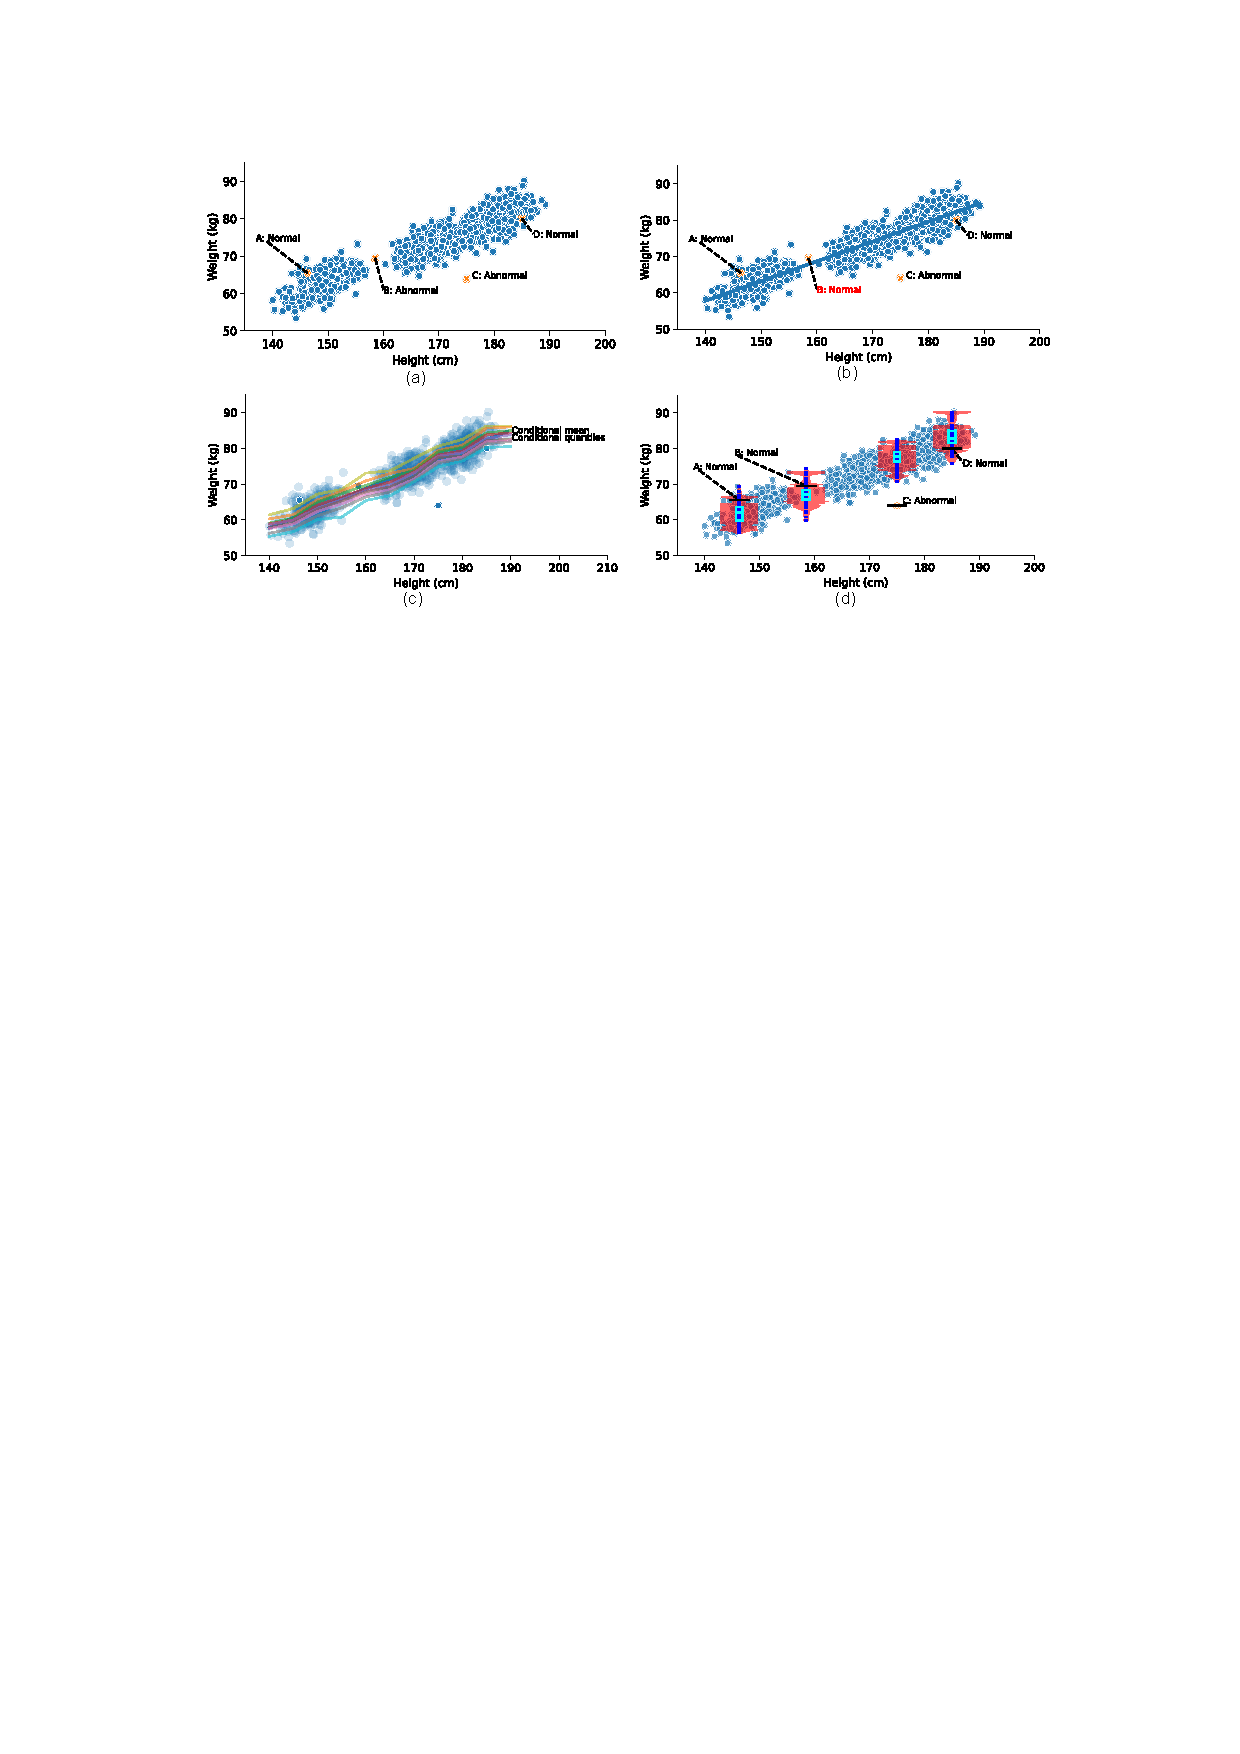
\includegraphics[width=12cm]{images/Pic_introduction.pdf}
\caption{Các loại phát hiện bất thường khác nhau. (a) Các phương pháp dựa trên khoảng cách và mật độ đều coi đối tượng B là bất thường, vì nó ở xa các đối tượng khác và ở vùng mật độ thấp. (b) Các phương pháp dựa trên sự phụ thuộc mô hình hóa mối quan hệ giữa chiều cao và cân nặng và do đó coi đối tượng B là bình thường. (c) Các phân vị có điều kiện cung cấp nhiều thông tin về phân bố có điều kiện hơn là chỉ giá trị trung bình và (d) có thể được sử dụng để trực quan hóa --- sử dụng biểu đồ beanplot (hoặc nói đúng hơn là một biến thể của biểu đồ beanplot kết hợp với biểu đồ hộp, xem Phần \ref{qcad:ae} để biết chi tiết) --- tại sao một đối tượng nhất định được coi là (ab)bình thường.}\label{fig:intro}
\end{figure}Các máy phát hiện bất thường nông thường được phân loại thành các phương pháp tiếp cận dựa trên khoảng cách, dựa trên mật độ và dựa trên phân phối \citep{wang2019progress}. Các phương pháp dựa trên khoảng cách và mật độ sử dụng kiến ​​thức về khoảng cách không gian của các đối tượng để xác định điểm bất thường, trong khi các phương pháp dựa trên phân phối sử dụng kiến ​​thức về phân bố dữ liệu để phát hiện điểm bất thường. Các phương pháp này hoạt động theo giả định rằng \textit{các đối tượng có khoảng cách lớn hoặc mật độ khác với các lân cận trong không gian của chúng là dị thường} hoặc \textit{các đối tượng có giá trị hiếm theo phân bố biên hoặc phân bố chung của các đặc điểm tương ứng là dị thường}. Tuy nhiên, việc sử dụng một trong hai giả định này có thể dẫn đến kết quả dương tính giả. Ví dụ: như trong Hình~\ref{fig:intro}(a), các phương pháp này sẽ xác định nhầm đối tượng B là vật thể dị thường nếu mục đích là phát hiện những người thừa cân hoặc thiếu cân.

Vì điều này thường không mong muốn nên chúng tôi muốn xác định và phát hiện các điểm bất thường từ một góc độ khác, nghĩa là chúng tôi giả định rằng \textit{các đối tượng vi phạm sự phụ thuộc, tức là mối quan hệ giữa các tính năng, là bất thường}. Đây là ý tưởng đằng sau tính năng phát hiện bất thường dựa trên phụ thuộc \citep{lu2020dependency}, ý tưởng này không mới nhưng nhận được sự chú ý hạn chế so với các loại dị thường khác. Nó tận dụng cấu trúc và thuộc tính nội tại của dữ liệu để tìm ra những điểm bất thường có khả năng phù hợp hơn. Ví dụ: Hình \ref{fig:intro}(b) cho thấy phương pháp này sẽ xác định đối tượng B là bình thường bằng cách mô hình hóa sự phụ thuộc giữa chiều cao và cân nặng.

Các kỹ thuật phát hiện điểm bất thường truyền thống --- bao gồm các phương pháp dựa trên khoảng cách, mật độ và sự phụ thuộc --- xử lý tất cả các đặc điểm như nhau khi xác định điểm bất thường. Tuy nhiên, trong các lĩnh vực như chăm sóc sức khỏe, mạng cảm biến và bảo vệ môi trường, một số tính năng không bao giờ được sử dụng trực tiếp để định lượng sự bất thường. Ví dụ, hệ thống phát hiện cháy rừng không nên coi các giá trị “sai lệch” của vĩ độ, kinh độ, ngày và giờ là dấu hiệu của sự bất thường. Tuy nhiên, chúng ta không nên đơn giản loại bỏ những tính năng này vì chúng có thể chứa thông tin liên quan. Ví dụ: nhiệt độ 'bình thường' có thể cao hơn ở một số vùng nhất định so với các vùng khác. Điều này thúc đẩy chúng tôi điều tra việc \emph{phát hiện bất thường theo ngữ cảnh}, vốn có thể có thể tính đến các tính năng bổ sung như vậy.

Tính năng phát hiện sự bất thường theo ngữ cảnh giả định rằng \textit{một đối tượng là bất thường nếu nó đi chệch hướng mạnh so với các đối tượng trong `ngữ cảnh' của các đối tượng tương tự}. Sự mâu thuẫn rõ ràng trong giả định này được giải thích bằng việc chia các đặc điểm thành hai tập con rời rạc, tức là các đặc trưng ngữ cảnh và các đặc trưng hành vi. Các đặc điểm ngữ cảnh chỉ được sử dụng để xác định bối cảnh, sử dụng một số thước đo tương tự, trong khi các đặc trưng hành vi chỉ được sử dụng để xác định xem một đối tượng có khác biệt với các đối tượng khác trong bối cảnh của nó hay không. Kiến thức về miền thường dẫn đến sự phân chia tự nhiên giữa các đặc điểm ngữ cảnh và hành vi.Chúng tôi nhận thấy rằng cả hai phương pháp phát hiện điểm bất thường dựa trên ngữ cảnh và dựa trên sự phụ thuộc đều xác định những điểm bất thường bằng cách khám phá sự phụ thuộc một cách rõ ràng hoặc ngầm giữa các tính năng. Cụ thể, các phương pháp phát hiện bất thường dựa trên sự phụ thuộc mô hình hóa mối quan hệ phụ thuộc giữa tất cả các tính năng một cách rõ ràng, trong khi các phương pháp phát hiện bất thường theo ngữ cảnh mô hình hóa mối quan hệ phụ thuộc giữa các đặc trưng hành vi và ngữ cảnh một cách ngầm định hoặc rõ ràng. Theo như chúng tôi biết thì mối liên hệ này vẫn chưa được chỉ ra trong tài liệu.

\smallskip \noindent
\textbf{Phương pháp tiếp cận và đóng góp}.

Trong bài viết này, chúng tôi giới thiệu một cách tiếp cận để phát hiện và giải thích sự bất thường theo ngữ cảnh tích hợp nguyên tắc cốt lõi của việc phát hiện sự bất thường dựa trên sự phụ thuộc vào việc phát hiện sự bất thường theo ngữ cảnh để có được một cách tiếp cận rất chính xác. Như thường lệ, chúng tôi sử dụng phân tích hồi quy để lập mô hình các phần phụ thuộc. Tuy nhiên, các phương pháp hiện có để phát hiện sự bất thường theo ngữ cảnh và dựa trên sự phụ thuộc sử dụng hồi quy thường chỉ ước tính giá trị trung bình có điều kiện của biến phản hồi và diễn giải trực tiếp giá trị đó là giá trị `bình thường'. Điều này hạn chế mạnh mẽ khả năng phát hiện các dị thường, vì giá trị trung bình có điều kiện cung cấp thông tin rất hạn chế về phân bố có điều kiện. Do đó, chúng tôi sử dụng \emph{hồi quy phân vị}, có thể lập mô hình phân phối có điều kiện chi tiết hơn nhiều bằng cách ước tính phân vị có điều kiện. Hình \ref{fig:intro}(c) cho thấy các phân vị có điều kiện cung cấp nhiều thông tin hơn về mối quan hệ giữa cân nặng và chiều cao như thế nào so với giá trị trung bình có điều kiện.

Cụ thể hơn, một tập hợp con các đặc điểm, được gọi là đặc điểm ngữ cảnh, được sử dụng để xác định bối cảnh của một đối tượng, trong khi các đặc điểm còn lại, được gọi là đặc trưng hành vi, được sử dụng để phát hiện những sai lệch trong một ngữ cảnh. Trong bài viết này, chúng tôi giả định rằng các đặc điểm ngữ cảnh có thể được trộn lẫn nhưng tất cả các đặc trưng hành vi đều là số. Dựa trên bối cảnh này và mục tiêu của chúng tôi, chúng tôi sử dụng Rừng hồi quy phân vị \citep{meinshausen2006quantile} để thực hiện dự đoán cho từng đặc trưng hành vi và thu được số lượng định lượng không chắc chắn tương ứng. Bằng cách tính tổng các độ không đảm bảo được định lượng (với khoảng lượng tử rộng hơn biểu thị mức độ không chắc chắn cao hơn) cho tất cả các đặc trưng hành vi riêng lẻ, chúng tôi thu được điểm bất thường cho một trường hợp dữ liệu. Bằng cách gán các phần của điểm bất thường cho các đặc trưng hành vi riêng lẻ, về bản chất, phương pháp này đưa ra những giải thích theo nghĩa là nó có thể truyền đạt ở mức độ nào các đặc điểm đã góp phần khiến cho trường hợp trở thành một điểm bất thường. Điều này mang lại lợi thế cho các phương pháp giải thích hậu nghiệm như SHAP \citep{lundberg2017unified}, mà chúng tôi không coi là 'có thể quy cho' vì hai lý do sau. Đầu tiên, lời giải thích hậu kiểm có thể không khớp với thông tin/lý do được mô hình sử dụng để phát hiện điểm bất thường \citep{li2022survey}. Thứ hai, gần đây \citep{fokkema2022attribution} đã chứng minh rằng các giải thích dựa trên thuộc tính không thể vừa nhạy cảm truy đòi vừa mạnh mẽ, đó là lý do chính đáng để tránh những giải thích như vậy khi có thể và thay vào đó hãy sử dụng phương pháp dựa trên phân bổ `bản địa'.Theo như chúng tôi biết, chúng tôi là những người đầu tiên sử dụng hồi quy phân vị để phát hiện sự bất thường theo ngữ cảnh hoặc dựa trên sự phụ thuộc. Cụ thể, chúng tôi chọn sử dụng Rừng hồi quy phân vị vì ba lý do. Đầu tiên, nó có thể mô hình hóa cả sự phụ thuộc tuyến tính và phi tuyến tính giữa các tính năng. Thứ hai, trong bài báo giới thiệu phương pháp này, qua thực nghiệm, nó đã được chứng minh là tốt hơn các công cụ ước tính phân vị có điều kiện khác trong hầu hết các trường hợp. Hình \ref{fig:intro}(d) cho thấy cách có thể sử dụng các phân vị có điều kiện ước tính để ước tính mật độ xác suất có điều kiện tại các vị trí khác nhau mà chúng ta có thể sử dụng để phát hiện chính xác các điểm bất thường. Hơn nữa, các lượng tử rất hữu ích để giải thích tại sao một đối tượng được coi là dị thường mà không cần phải đề cập rõ ràng đến các đối tượng khác.


Những đóng góp chính trong công việc của chúng tôi có thể được tóm tắt như sau: (1) Chúng tôi xác định mối liên hệ giữa các phương pháp phát hiện sự bất thường truyền thống dựa trên sự phụ thuộc và các phương pháp phát hiện sự bất thường theo ngữ cảnh, đồng thời khai thác quan sát này để giới thiệu một cách tiếp cận cấp cao mới để phát hiện và giải thích sự bất thường theo ngữ cảnh; (2) Chúng tôi khởi tạo cách tiếp cận chung này bằng cách sử dụng hồi quy phân vị (và cụ thể là Rừng hồi quy phân vị) để phát hiện sự bất thường và trực quan hóa dựa trên Beanplot để giải thích sự bất thường; và (3) Chúng tôi thực hiện các thử nghiệm sâu rộng trên các bộ dữ liệu tổng hợp và trong thế giới thực để chứng minh bằng thực nghiệm tính hiệu quả và khả năng diễn giải của phương pháp được đề xuất khi so sánh với các phương pháp hiện đại.

Phần còn lại của bài viết này được tổ chức như sau. Phần 2 thảo luận về công việc liên quan, cả về phát hiện sự bất thường theo ngữ cảnh và truyền thống. Phần 3 giới thiệu ký hiệu, hình thức hóa bài toán và trình bày cách tiếp cận cấp cao mà chúng tôi đề xuất. Phần 4 sau đó mô tả một số kỹ thuật sơ bộ, đáng chú ý nhất là Rừng hồi quy phân vị. Phần 5 giới thiệu QCAD, phương pháp được đề xuất của chúng tôi để Phát hiện và giải thích bất thường theo ngữ cảnh dựa trên lượng tử nhằm khởi tạo cách tiếp cận cấp cao. Phần 6 so sánh QCAD với các đối thủ cạnh tranh theo kinh nghiệm và cung cấp một nghiên cứu điển hình điều tra việc sử dụng QCAD để tìm các cầu thủ bóng đá xuất sắc từ dữ liệu. Phần 7 kết luận bài viết.
\section{Công việc liên quan}
\label{sec:relatedWork}

Trước tiên, chúng tôi thảo luận về công việc liên quan về phát hiện và giải thích bất thường theo ngữ cảnh, sau đó tiến hành hai loại phát hiện bất thường truyền thống có liên quan chặt chẽ nhất: phát hiện bất thường dựa trên phụ thuộc và dựa trên không gian con.

\subsection{Phát hiện và giải thích sự bất thường theo ngữ cảnh}

Phát hiện bất thường theo ngữ cảnh đã nhận được sự chú ý đặc biệt trong dữ liệu không gian \citep{cai2013spatial}, dữ liệu thời gian \citep{salvador2004learning} và dữ liệu không gian-thời gian \citep{smets2009discovering}, trong đó các đặc điểm không gian và/hoặc thời gian được sử dụng để xác định bối cảnh. Các phương pháp này không thể áp dụng trực tiếp cho các miền khác, trong đó bối cảnh được xác định bởi các loại đối tượng địa lý khác; Phát hiện bất thường theo ngữ cảnh 'chung' đã nhận được sự quan tâm hạn chế trong cộng đồng.

CAD \citep{song2007conditional} là một công trình quan trọng giới thiệu tính năng phát hiện bất thường theo ngữ cảnh chung. Nó giả định một phân vùng các tính năng do người dùng chỉ định thành các đặc trưng ngữ cảnh (được gọi là 'môi trường') và hành vi (được gọi là 'chỉ báo'), đồng thời sử dụng Mô hình hỗn hợp Gaussian để phù hợp với sự phân bố của các không gian đặc trưng ngữ cảnh và hành vi. Sự phụ thuộc giữa các đặc điểm ngữ cảnh và đặc trưng hành vi sau đó được học bằng 'các hàm ánh xạ' và một đối tượng được coi là bất thường nếu nó vi phạm các hàm đã học. Để điều này hoạt động, CAD giả định rằng cả đặc điểm ngữ cảnh và hành vi đều bao gồm một số lượng không xác định của nhiều thành phần Gaussian, đây có thể là một giả định chắc chắn trong thực tế. Hơn nữa, CAD chỉ có thể xử lý các tính năng số và rất tốn kém về mặt tính toán. Phương pháp được đề xuất của chúng tôi không đưa ra giả định nào về việc phân phối các tính năng, có thể xử lý các đặc trưng ngữ cảnh hỗn hợp và các đặc trưng hành vi số và chúng tôi sẽ chứng minh bằng thực nghiệm rằng nó hiệu quả hơn về mặt tính toán so với CAD trong khi đạt được độ chính xác phát hiện cao hơn.

ROCOD \citep{liang2016robust} cũng có liên quan chặt chẽ và sử dụng các mô hình hành vi dự kiến ​​cục bộ và toàn cầu để mô tả sự phụ thuộc giữa các đặc trưng ngữ cảnh và hành vi. Cụ thể, các mô hình hồi quy tiêu chuẩn như CART được sử dụng để tìm hiểu các mô hình toàn cầu, với các đặc trưng ngữ cảnh là các biến dự đoán và các đặc trưng hành vi là các biến phản hồi. Các mẫu cục bộ được tính toán dựa trên phương tiện giá trị đặc trưng hành vi của các láng giềng của đối tượng. Giá trị thực tế của một đối tượng được so sánh với mô hình cục bộ và tổng thể, và mức trung bình có trọng số của những khác biệt này tạo thành điểm bất thường. Vì giá trị trung bình có điều kiện chỉ mô tả một khía cạnh của phân bố có điều kiện và không nhất thiết là điểm có xác suất xảy ra cao nhất (tức là chế độ). Để giải quyết vấn đề này, phương pháp của chúng tôi sử dụng phân tích hồi quy phân vị để ước tính các phân vị có điều kiện, cung cấp mô tả đầy đủ hơn về phân bố có điều kiện. Kết quả là, phương pháp của chúng tôi về mặt thực nghiệm vượt trội hơn ROCOD về độ chính xác.Với việc sử dụng ngày càng nhiều các thuật toán phát hiện sự bất thường trong các lĩnh vực quan trọng về an toàn, chẳng hạn như chăm sóc sức khỏe và sản xuất, nghĩa vụ đạo đức và quy định trong việc đưa ra lời giải thích cho các quyết định mang tính rủi ro cao do các thuật toán này đưa ra đã trở nên rõ ràng hơn \citep{li2022survey}. Tuy nhiên, tính năng phát hiện bất thường theo ngữ cảnh hiện tại không đưa ra những giải thích như vậy và sẽ cần có những sửa đổi không hề nhỏ để thực hiện điều đó. Cụ thể, CAD \citep{song2007conditional} tính toán điểm bất thường của một phiên bản dữ liệu bằng cách đo độ lệch của nó so với các hàm ánh xạ được học từ phần lớn các phiên bản dữ liệu. Cách tiếp cận này đặt ra thách thức trong việc tạo ra các giải thích nội tại, vì nó không cho phép quy kết điểm bất thường cho các đặc điểm riêng lẻ. Hơn nữa, ROCOD \citep{liang2016robust}, một phương pháp được biết đến khác để phát hiện điểm bất thường theo ngữ cảnh, tính toán mức trung bình có trọng số của sự khác biệt của một phiên bản với các mẫu cục bộ và toàn cầu đã học dưới dạng điểm bất thường của nó. Mẫu cục bộ được lấy bằng cách sử dụng các mẫu lân cận của nó, trong khi mẫu chung được học bằng cách sử dụng tất cả các trường hợp, khiến việc liên kết điểm bất thường với các đặc điểm riêng lẻ trở nên khó khăn.

Bất chấp sự tồn tại của nhiều phương pháp để giải thích các dị thường, chẳng hạn như những phương pháp được nêu trong các bài báo (khảo sát) gần đây \citep{panjei2022survey,li2022survey,xu2021beyond}, vẫn có rất ít nghiên cứu về cách giải thích các bất thường theo ngữ cảnh. Đặc biệt, COIN \citep{liu2018contextual} giải thích các ngoại lệ bằng cách báo cáo điểm ngoại lệ của chúng, các đặc điểm góp phần tạo ra sự bất thường của nó và mô tả theo ngữ cảnh của các vùng lân cận. Tuy nhiên, COIN xử lý tất cả các tính năng như nhau, trong khi phương pháp của chúng tôi chia các tính năng thành các đặc trưng ngữ cảnh và hành vi. Hơn nữa, chúng tôi phát triển một hình ảnh trực quan giúp giải thích các điểm bất thường theo ngữ cảnh bên cạnh việc báo cáo điểm bất thường tổng thể, tầm quan trọng của đối tượng địa lý, các lân cận theo ngữ cảnh và điểm bất thường riêng lẻ cho từng đặc trưng hành vi.



Các phương pháp sau đây ít liên quan hơn vì chúng xem xét các vấn đề hơi khác nhau. \cite{valko2011conditional} xây dựng một phương pháp dựa trên biểu đồ phi tham số để phát hiện sự bất thường có điều kiện, phương pháp này chỉ giải quyết vấn đề về một đặc trưng hành vi phân loại duy nhất. \cite{hayes2014contextual} trước tiên xác định các điểm bất thường trên các đặc trưng hành vi, sau đó tinh chỉnh các điểm bất thường được phát hiện bằng cách phân cụm tất cả các đối tượng trên các đặc trưng ngữ cảnh. \cite{tang2015mining} phát hiện các điểm bất thường của nhóm từ dữ liệu phân loại đa chiều.  \cite{hong2015multivariate} trình bày một khung phát hiện bất thường theo ngữ cảnh dành riêng cho các đặc trưng hành vi phân loại, khung này cũng xem xét sự phụ thuộc giữa các đặc trưng hành vi. Hơn nữa, \cite{zheng2017contextual} áp dụng phương pháp học số liệu mạnh mẽ trên các đặc trưng ngữ cảnh để tìm các lân cận theo ngữ cảnh có ý nghĩa hơn và sau đó tận dụng hồi quy hạt nhân $k$-NN để dự đoán các giá trị đặc trưng hành vi. \cite{meghanath2018conout} phát triển ConOut để tự động tìm và kết hợp nhiều bối cảnh nhằm xác định và giải thích các ngoại lệ.


\subsection{Phát hiện bất thường truyền thống}Mặc dù phát hiện bất thường truyền thống coi một vấn đề khác với phát hiện bất thường theo ngữ cảnh, các kỹ thuật tận dụng phát hiện bất thường dựa trên phụ thuộc và dựa trên không gian con có liên quan đến phương pháp của chúng tôi.

\subsubsection{Phát hiện bất thường dựa trên phụ thuộc}
Tính năng phát hiện bất thường dựa trên phần phụ thuộc nhằm mục đích xác định các điểm bất thường bằng cách khám phá các phần phụ thuộc giữa các tính năng. \cite{teng1999correcting} khám phá sự phụ thuộc giữa các tính năng không phải mục tiêu và mục tiêu để xác định và sửa các điểm dữ liệu nhiễu có thể xảy ra. Để phát hiện các hành vi xâm nhập mạng, \cite{huang2003cross} trình bày Phân tích tính năng chéo để nắm bắt các mẫu phụ thuộc giữa các tính năng trong lưu lượng mạng thông thường. Để phát hiện sự bùng phát dịch bệnh, \cite{wong2003bayesian} đề xuất khám phá sự phụ thuộc giữa các tính năng bằng mạng Bayesian. \cite{noto2010anomaly} đề xuất phát hiện các điểm bất thường bằng cách sử dụng một tập hợp các mô hình, trong đó mỗi mô hình khám phá sự phụ thuộc giữa tính năng phản hồi và các tính năng khác. \cite{babbar2012mining} sử dụng mạng Bayesian Gaussian tuyến tính để phát hiện những điểm bất thường vi phạm mối quan hệ nhân quả.

LoPAD \citep{lu2020lopad} trước tiên sử dụng mạng Bayesian để tìm Chăn Markov của từng tính năng. Sau đó, một mô hình dự đoán (ví dụ: GIỎ HÀNG) được học cho từng tính năng riêng lẻ dưới dạng biến phản hồi, với Chăn Markov của nó làm biến dự đoán. Với một đối tượng, LoPAD tính toán khoảng cách Euclide giữa giá trị thực tế và giá trị dự đoán (tức là giá trị trung bình có điều kiện) làm điểm bất thường cho từng đối tượng. Điểm bất thường thu được được chuẩn hóa và tính tổng để có được điểm bất thường cuối cùng cho một đối tượng. Phương pháp này không phân biệt các đặc trưng ngữ cảnh và hành vi và --- giống như ROCOD --- sử dụng các phương tiện có điều kiện để biểu diễn phân bố có điều kiện. Do đó, LoPAD không thể (chính xác) phát hiện các điểm bất thường theo ngữ cảnh.

\subsubsection{Phát hiện bất thường dựa trên không gian con}
Phát hiện dị thường dựa trên không gian con tìm cách tìm ra các dị thường trong một phần của không gian đặc trưng. Cụ thể, \cite{kriegel2009outlier} đề xuất SOD để xác định các ngoại lệ trong các không gian con khác nhau. Cụ thể, họ xây dựng các không gian con trục song song được kéo dài bởi các lân cận của một đối tượng nhất định. Trên cơ sở này, họ điều tra xem liệu đối tượng này có sai lệch đáng kể so với các đối tượng lân cận của nó trên bất kỳ không gian con nào trong số này hay không. Hơn nữa, \cite{kriegel2012outlier} mở rộng công việc này để xác định xem một đối tượng có bất thường trên các không gian con được định hướng tùy ý bao quanh các không gian lân cận của nó hay không. \cite{nguyen2013cmi} đề xuất tìm các không gian con có mối tương quan chặt chẽ với nhau và sau đó xác định các điểm bất thường trên các không gian con này. Cuối cùng, \cite{cabero2021archetype} sử dụng phân tích nguyên mẫu để chiếu không gian đặc trưng vào các không gian con khác nhau với các mối tương quan tuyến tính dựa trên các lân cận gần nhất. Trên cơ sở này, họ khám phá các giá trị ngoại lệ bằng cách tập hợp các kết quả thu được trên các không gian con có liên quan. Nhìn chung, các phương pháp này nhằm mục đích xác định các điểm bất thường trong một tập hợp con các đặc điểm, nhưng xử lý tất cả các đặc điểm một cách bình đẳng và do đó không phù hợp để xác định các điểm bất thường theo ngữ cảnh.
\section{Phát hiện và giải thích sự bất thường theo ngữ cảnh}
\label{sec:framework}

Trước tiên, chúng tôi giới thiệu các thuật ngữ và ký hiệu cần thiết, đồng thời minh họa điều này bằng ví dụ chạy được mô tả trong Bảng~\ref{tab:ExampleData}. Tập dữ liệu $\mathbf{X} =\{\mathbf{x}_{1},\ldots,\mathbf{x}_{i},\ldots,\mathbf{x}_{N}\}$ chứa các phiên bản $N$ (hoặc điểm dữ liệu) trên tập hợp các tính năng (còn gọi là thuộc tính hoặc biến) được biểu thị bằng $\mathbf{F} = \{\mathbf{f}^{1},\ldots,\mathbf{f}^{j},\ldots,\mathbf{f}^{D}\}$. $x_{i}^{j}$ biểu thị giá trị của đối tượng thứ $i$, $\mathbf{x}_{i}$, cho tính năng thứ $j$, $\mathbf{f}^{j}$. Trong ví dụ đang chạy, chúng ta có $N=16$, $D=6$, $\mathbf{F}= \{Latitude, Longitude, Season, Temperature, Rain, Wind\}$ và $x_{1}^{Rain} = 69$.

\begin{table}[!htbp]
\caption{Ví dụ đang chạy: dữ liệu khí hậu hư cấu cho các thành phố của Hà Lan. Nhiệt độ được đo bằng độ C, mưa tính bằng mm và gió tính bằng dặm một giờ. Thành phố không được sử dụng để phát hiện sự bất thường. \emph{Latitude}, \emph{Kinh độ} và \emph{Mùa} được coi là các đặc trưng ngữ cảnh, trong khi \textbf{Nhiệt độ}, \textbf{Mưa} và \textbf{Gió} được coi là hành vi tính năng.}\label{tab:ExampleData}
\begin{center}
\begin{tabular}{cccccccc}
\toprule
Thành phố & \emph{Vĩ độ} & \emph{Kinh độ} & \emph{Mùa} & \textbf{Nhiệt độ} & \textbf{Mưa} & \textbf{Gió}\\
\midrule
Leiden & 52.16 & 4.49 & Mùa đông & 3.0 & 69 & 16\\
Amsterdam & 52.37 & 4.89 & Mùa đông & 2.9 & 55 & 17\\
Rotterdam & 51.92 & 4.46 & Mùa đông & 2.7 & 60 & 15\\
Oss & 51.45 & 5.31 & Mùa đông & 1.1 & 58 & 25\\
Eindhoven & 51.44 & 5.46 & Mùa Thu & 16.6 & 62 & 25\\
Delft & 52.00 & 4.21 & Mùa Thu & 16.1 & 45 & 19\\
Utrecht & 52.09 & 5.10 & Mùa Thu & 18.3 & 42 & 20\\
The Hague & 52.07 & 4.28 & Mùa Thu & 18.5 & 49 & 18\\
Tilburg & 51.33 & 5.52 & Mùa hè & 22.1 & 39 & 22\\
Middelburg & 51.49 & 3.61 & Mùa hè & 20.3 & 41 & 23\\
Arnhem & 51.98 & 5.89 & Mùa hè & 19.6 & 48 & 17\\
Venlo & 51.37 & 6.17 & Mùa hè & 21.8 & 43 & 35\\
Emmen & 52.46 & 6.55 & Mùa Xuân & 8.3 & 80 & 10\\
Meppel & 52.69 & 6.19 & Mùa Xuân & 7.1 & 27 & 13\\
Groningen & 53.13 & 6.34 & Mùa xuân & 4.2 & 17 & 19\\
Leeuwarden & 53.10 & 5.80 & Mùa Xuân & 7.2 & 17 & 19\\
\botrule
\end{tabular}
\end{center}
\end{table}Chúng tôi giả định rằng bộ tính năng $\mathbf{F}$ được chia thành hai bộ tính năng riêng biệt (thường sử dụng kiến ​​thức về miền): bộ đặc trưng ngữ cảnh $\mathbf{C} =\{\mathbf{c}^{1},...,\mathbf{c}^{p},\ldots,\mathbf{c}^{P}\}$ và bộ đặc trưng hành vi $\mathbf{B} =\{\mathbf{b}^{1},\ldots,\mathbf{b}^{q},\ldots,\mathbf{b}^{Q}\}$, chẳng hạn như $D=P+Q$, $\mathbf{F} = \mathbf{C} \cup \mathbf{B}$ và $\mathbf{C} \cap \mathbf{B} = \emptyset$. Không mất tính tổng quát, ta có thể sắp xếp lại đặc điểm của đối tượng
$\mathbf{x}_{i}=(x_{i}^{1},...,x_{i}^{j},...,x_{i}^{D})$ và biểu thị nó dưới dạng $\mathbf{x}_{i}=(x_{i}^{1},...,x_{i}^{P},x_{i}^{P+1},...,x_{i}^{P+Q}) = (c_{i}^{1},...,c_{i}^{p},...,c_{i}^{P},b_{i}^{1},...,b_{i}^{q},...,b_{i}^{Q})=(\mathbf{c}_{i}, \mathbf{b}_{i}) $, do đó $\mathbf{c}_{i}$ và $\mathbf{b}_{i}$ lần lượt biểu thị các giá trị đặc trưng ngữ cảnh và hành vi của nó. Theo đó, chúng tôi gọi không gian được kéo dài bởi $\mathbf{C}$ là \textit{không gian ngữ cảnh}, tức là $\mathcal{C} = \mathbf{c}^{1}\times... \times\mathbf{c}^{p}\times...\times\mathbf{c}^{P}$ và không gian được kéo dài bởi $\mathbf{B}$ là \textit{không gian hành vi}, tức là $\mathcal{B} = \mathbf{b}^{1}\times...\times \mathbf{b}^{q}\times...\times\mathbf{b}^{Q}$.

Cuối cùng, đặt $\Pow$ biểu thị tập lũy thừa, tức là $\Pow(\mathbf{X}) = \{X \subseteq \mathbf{X}\}$.

\subsection{Báo cáo vấn đề}

Khi phát hiện sự bất thường theo ngữ cảnh, các đặc trưng ngữ cảnh được sử dụng để xác định cái gọi là \emph{bối cảnh} của một đối tượng. Bối cảnh của một đối tượng được sử dụng để ước tính liệu nó có bất thường hay không. Điều thứ hai đạt được bằng cách so sánh các giá trị của đối tượng về các đặc trưng hành vi với những gì là `bình thường' trong ngữ cảnh của đối tượng --- nếu các giá trị hành vi của đối tượng sai lệch mạnh, nó sẽ bị gắn cờ là bất thường.

Để phát hiện sự bất thường theo ngữ cảnh có ý nghĩa, chúng ta phải giả định rằng \emph {tồn tại sự phụ thuộc giữa dữ liệu theo ngữ cảnh và hành vi}. Nếu mối quan hệ như vậy không tồn tại thì không cần sử dụng tính năng phát hiện sự bất thường theo ngữ cảnh; người ta có thể chỉ cần loại bỏ các đặc trưng ngữ cảnh và giảm vấn đề thành vấn đề phát hiện sự bất thường truyền thống.

Chúng tôi minh họa điều này bằng ví dụ đang chạy trong Bảng~\ref{tab:ExampleData}. Chúng tôi có thể phát hiện thời tiết bất thường có tính đến các khu vực và mùa khác nhau bằng cách chỉ định bộ đặc trưng ngữ cảnh $\mathbf{C} = \{Latitude, Longitude, Season\}$ và bộ đặc trưng hành vi $\mathbf{B} = \{Temperature, Rain, Wind\}$. Mỗi thành phố hiện chỉ được so sánh với các thành phố có cùng vĩ độ, kinh độ và mùa, tức là bối cảnh của nó. Nếu một thành phố có các giá trị về nhiệt độ, mưa và/hoặc gió khác xa nhiều so với các giá trị của thành phố trong bối cảnh của nó thì thành phố đó được đánh dấu là bất thường.

Ví dụ, Amsterdam và Rotterdam có thể tạo thành bối cảnh của Leiden; cả hai đều ở gần và chúng tôi có số đo cho cùng một mùa. Nhiệt độ và gió ở cả ba thành phố đều giống nhau, nhưng ở Leiden về cơ bản có lượng mưa nhiều hơn ở Amsterdam và Rotterdam. Do đó, vì lý do đó Leiden có thể bị coi là một kẻ dị thường.Để chính thức hóa vấn đề, chúng tôi giới thiệu một `hàm ngữ cảnh' chung để ánh xạ từng điểm dữ liệu có thể có vào một tập hợp con của tập dữ liệu, tức là ngữ cảnh của nó, dựa trên các đặc điểm ngữ cảnh của điểm dữ liệu.

\textbf{Vấn đề 1: Phát hiện bất thường theo ngữ cảnh} Cho một tập dữ liệu $\mathbf{X}$ với bộ tính năng $\mathbf{F} = (\mathbf{C},\mathbf{B})$, hàm ngữ cảnh $\context : \mathcal{C} \rightarrow \Pow(\mathbf{X})$, trình phát hiện bất thường $\anomaly : \mathcal{B} \times \Pow(\mathbf{X}) \rightarrow \mathbb{R}^{+}$ và ngưỡng $\phi$, tìm tất cả các điểm dữ liệu cho điểm bất thường vượt quá $\phi$ và do đó được gắn cờ là bất thường---dựa trên các đặc trưng hành vi---trong bối cảnh riêng của chúng, tức là $\{(\mathbf{c},\mathbf{b}) \in \mathbf{X} \mid \anomaly(\mathbf{b}, \context(\mathbf{c})) \geq \phi \}$.

Lưu ý rằng bối cảnh chỉ được xác định dựa trên các giá trị đặc trưng ngữ cảnh và trình phát hiện bất thường chỉ có thể sử dụng các giá trị đặc trưng hành vi của các điểm dữ liệu trong ngữ cảnh nhất định khi xác minh xem điểm dữ liệu đã cho có bất thường hay không.

Trong thực tế, các nhà phân tích không chỉ quan tâm đến việc xác định các điểm bất thường mà còn cần biết lý do cơ bản tại sao một đối tượng cụ thể được báo cáo là bất thường. Điều này dẫn đến vấn đề thứ hai mà chúng tôi xem xét.

\textbf{Vấn đề 2: Giải thích bất thường theo ngữ cảnh} Cho một đối tượng dị thường $\mathbf{x} \in \mathbf{X}$ và hàm ngữ cảnh $\context$ và trình phát hiện bất thường $\anomaly$ đã được sử dụng để phát hiện nó, hãy tìm các đặc trưng hành vi $\mathbf{B'} \subseteq \mathbf{B}$ để ứng phó $\mathbf{x} = (\mathbf{c}, \mathbf{b})$ khác biệt đáng kể so với $\context(\mathbf{c})$.

\subsection{Phương pháp tiếp cận tổng thể} \label{subsec:framework}

Báo cáo vấn đề trong phần trước gợi ý cách tiếp cận ba hướng dựa trên việc tạo bối cảnh 1), phát hiện bất thường 2) và giải thích bất thường 3). Trong tiểu mục này, chúng tôi giải thích và minh họa cách tiếp cận tổng thể mà chúng tôi đề xuất, sử dụng ví dụ đang chạy từ Bảng~\ref{tab:ExampleData}.

\begin{figure}[!htbp]
\centering
\includegraphics[width=12cm]{images/Pic_framework.pdf}
\caption{ Giải thích về sự bất thường và tạo nhóm tham chiếu. Giai đoạn Tạo nhóm tham chiếu tính toán ma trận khoảng cách chỉ sử dụng các đặc trưng ngữ cảnh và tìm nhóm tham chiếu cho từng đối tượng trên cơ sở này.  Giai đoạn Giải thích sự bất thường tạo ra lời giải thích cho từng điểm bất thường được xác định bằng cách báo cáo các điểm bất thường lân cận theo ngữ cảnh, điểm bất thường cuối cùng và điểm bất thường thô trong từng đặc trưng hành vi.}\label{fig:framework}
\end{figure}

\paragraph{Giai đoạn 1: Tạo nhóm tham chiếu} Có thể có nhiều lựa chọn cho hàm ngữ cảnh; trong bản thảo này, chúng tôi chọn sử dụng hàng xóm gần nhất $k$ của một đối tượng mà chúng tôi gọi là \emph{nhóm tham chiếu}. Lý do quan trọng nhất cho sự lựa chọn này là 1) khi ma trận khoảng cách theo ngữ cảnh toàn cầu đã được tính toán, các lân cận gần nhất của bất kỳ đối tượng nào có thể được tìm thấy tương đối nhanh chóng; 2) phương pháp này chỉ yêu cầu chọn số liệu khoảng cách, số liệu này có thể được xác định cho bất kỳ loại dữ liệu nào và được điều chỉnh cho phù hợp với vấn đề hiện tại; và 3) nó đủ chung để cho phép sử dụng các bối cảnh kết quả khác nhau.Cho một tập dữ liệu $\mathbf{X}$ với bộ đặc trưng ngữ cảnh $\mathbf{C}$, trước tiên chúng tôi tính toán ma trận khoảng cách $\mathbf{M}$ giữa tất cả các đối tượng chỉ sử dụng các đặc trưng ngữ cảnh. Thứ hai, đối với bất kỳ đối tượng $\mathbf{x} \in \mathbf{X}$ nào, chúng tôi tìm thấy $k$ lân cận gần nhất của nó trong \textit{không gian ngữ cảnh} dựa trên $\mathbf{M}$. Kết quả là, $k$ lân cận gần nhất của $\mathbf{x}$ tạo thành một nhóm tham chiếu, được ký hiệu là $R(\mathbf{x},k)$, đóng vai trò là bối cảnh trong các Sự cố 1 và 2.

Ví dụ, như trong Hình \ref{fig:framework} (a), cho $\{Latitude, Longitude, Season\}$ làm tập đặc điểm ngữ cảnh, trước tiên chúng ta tính toán ma trận khoảng cách trong không gian ngữ cảnh $Latitude \times Longitude \times Season$. Thứ hai, dựa trên ma trận khoảng cách, chúng ta có thể tìm thấy ba lân cận gần nhất của bất kỳ đối tượng nào làm nhóm tham chiếu\footnote{Chúng tôi sử dụng $k=3$ cho mục đích minh họa; trong thực tế, chúng tôi sẽ có một tập dữ liệu có nhiều hơn các bản ghi 16 và $k$ cũng sẽ lớn hơn nhiều.}. Cụ thể, ba láng giềng gần nhất của $\mathbf{x}_{1}$ là $\{\mathbf{x}_{2},\mathbf{x}_{3},  \mathbf{x}_{4}\}$, tạo thành một nhóm tham chiếu cho $\mathbf{x}_{1}$, ký hiệu là $R(\mathbf{x}_{1},3)$.

\paragraph{Phase 2: Phát hiện bất thường} Với một đối tượng $\mathbf{x} \in \mathbf{X}$ với nhóm tham chiếu $R(\mathbf{x},k)$, chúng tôi áp dụng trình phát hiện bất thường $\anomaly$ để đạt được điểm bất thường \emph{chỉ dựa trên các giá trị thuộc tính hành vi}. Chúng tôi lặp lại quy trình trên cho tất cả các đối tượng, dẫn đến điểm bất thường của $N$ là $S= \{s_{1},s_{2},...,s_{N}\}$. Chúng tôi sắp xếp $S$ và sử dụng ngưỡng $\phi$ để có được danh sách xếp hạng các điểm bất thường theo ngữ cảnh $A= \{\mathbf{a}_{1},...,\mathbf{a}_{m},...,\mathbf{a}_{M}\}$, với $M \ll N$.

Ví dụ: chúng ta có thể áp dụng trình phát hiện bất thường trên \textit{không gian hành vi} $Temperature \times Rain \times Wind$ của $\mathbf{x}_{1}$ và nhóm tham chiếu $R(\mathbf{x}_{1},3)=\{\mathbf{x}_{2},\mathbf{x}_{3},\mathbf{x}_{4}\}$ của nó. Kết quả là chúng tôi thu được điểm bất thường $s_{1}$ cho $\mathbf{x}_{1}$. Theo đó, việc lặp lại quá trình này sẽ dẫn đến một tập hợp điểm bất thường $S= \{s_{1},...,s_{16}\}$. Trong ví dụ đang chạy, chúng tôi thấy $\{\mathbf{x}_{4},\mathbf{x}_{12},\mathbf{x}_{13}\}$ là các điểm bất thường theo ngữ cảnh, vì chúng hoạt động khác nhau trong không gian hành vi $Temperature \times Rain \times Wind$ khi so sánh với các lân cận tương ứng của chúng được xác định trong không gian ngữ cảnh $Latitude \times Longitude \times Season$. Ví dụ, Oss ($\mathbf{x}_{4}$) có gió tương đối mạnh hơn vào mùa đông khi so sánh với các thành phố gần nhất là Leiden, Amsterdam và Rotterdam.

Chúng tôi yêu cầu trình phát hiện bất thường phải là \textit{có thể phân bổ}, nghĩa là điểm bất thường $s$ do trình phát hiện bất thường tạo ra phải có thể phân tách thành các đóng góp riêng lẻ đối với tính bất thường cho từng đặc trưng hành vi bằng cách sử dụng cấu trúc gốc của trình phát hiện bất thường.\paragraph{Giai đoạn 3: Giải thích bất thường} Đối với mỗi đối tượng dị thường $\mathbf{a}_{m}$, trước tiên chúng tôi báo cáo nhóm tham chiếu $R(\mathbf{a}_{m},k)$ của nó bằng cách sử dụng ma trận khoảng cách thu được trong Giai đoạn $1$. Thứ hai, chúng tôi báo cáo điểm bất thường $s_{m}$ của nó, như thu được trong Giai đoạn $2$. Hơn nữa, chúng tôi phân tách $s_{m}$ thành các đóng góp riêng lẻ từ mỗi đặc trưng hành vi $\mathbf{b}^{q} \in \mathbf{B}$, dẫn đến danh sách các điểm bất thường thô $\mathbf{s}_{m}=\{s_{m1},...,s_{mq},...,s_{mQ}\}$. Điều này có thể thực hiện được vì $s_{m}$ là \emph{thuộc tính}. Tiếp theo, chúng tôi báo cáo điểm bất thường thô $h$ hàng đầu trong $\mathbf{s}_{m}$ với các đặc trưng hành vi tương ứng của chúng, trong đó nhà phân tích có thể chỉ định $h$. Các đặc trưng hành vi và điểm thô hàng đầu của $h$ cho phép các nhà phân tích hiểu rõ hơn lý do tại sao một đối tượng cụ thể được gắn cờ là bất thường theo ngữ cảnh.

Ví dụ: Hình \ref{fig:framework} (b) báo cáo đối tượng $\mathbf{x}_{12}$ là một điểm bất thường. Để giải thích lý do, trước tiên chúng tôi kiểm tra nhóm tham chiếu $R(\mathbf{x}_{12},3)=\{\mathbf{x}_{10},\mathbf{x}_{11},\mathbf{x}_{12}\}$ của nó, nhóm này chứa ba đối tượng giống với $\mathbf{x}_{12}$ nhất. Thứ hai, chúng tôi báo cáo điểm bất thường của nó, tức là $90$. Tiếp theo, chúng tôi phân tách điểm số và báo cáo các đặc trưng hành vi có độ lệch cao nhất, ví dụ: $Wind$. Chúng ta có thể hiểu kết quả là: $\mathbf{x}_{12}$ sai lệch đáng kể trong $Wind$ khi so sánh với $\{\mathbf{x}_{10},\mathbf{x}_{11},\mathbf{x}_{12}\}$, tất cả đều giống nhau về $Latitude$, $Longitude$ và $Season$.

\section{Vòng sơ loại}
\label{sec:prelim}

Trước tiên, chúng tôi xác định giá trị trung bình có điều kiện và phân vị có điều kiện mà chúng tôi sử dụng để thúc đẩy việc sử dụng phân vị có điều kiện để phát hiện sự bất thường. Tiếp theo, chúng tôi trình bày chi tiết về các khu rừng hồi quy phân vị, một lớp mô hình có thể ước tính mạnh mẽ các phân vị có điều kiện. Độc giả quen thuộc với những khái niệm này có thể bỏ qua phần này.


\subsection{Từ trung bình có điều kiện đến phân vị có điều kiện}
\label{subsec:meantoquantiles}

Cho một biến $V$ có giá trị thực và một tập hợp các biến $\mathbf{U}$, phân tích hồi quy nhằm mục đích lập mô hình phân phối $V$ dựa trên $\mathbf{U}$. Cụ thể, phải lấy $V$ làm biến phản hồi và $\mathbf{U}$ làm biến dự đoán để xây dựng một mô hình có thể dùng để dự đoán $V$ dựa trên $\mathbf{U}$.
Hồi quy tiêu chuẩn sử dụng dữ liệu huấn luyện $\{(\mathbf{U}_{1},V_{1}),...,(\mathbf{U}_{n},V_{n})\}$ để tìm hiểu mô hình ước tính giá trị trung bình có điều kiện $E(V \mid \mathbf{U}=\mathbf{u})$ và sử dụng dữ liệu đó làm dự đoán cho $V$ khi $\mathbf{U}=\mathbf{u}$ được đưa ra. Ví dụ: Hồi quy bình phương tối thiểu phù hợp với mô hình $\hat{\theta}$ bằng cách giảm thiểu tổn thất lỗi bình phương dự kiến, cụ thể là $\hat{\theta} =  \underset{\theta}{\mathrm{argmin}}\, E\{(V-\hat{V}(\theta))^{2})\mid \mathbf{U}=\mathbf{u}\}$.

Tuy nhiên, giá trị trung bình có điều kiện chỉ là một thống kê duy nhất của phân bố có điều kiện và do đó bị giới hạn về những gì nó có thể nắm bắt được. Ví dụ: nếu phân phối có điều kiện là phân phối đa phương thức thì giá trị trung bình không đủ để mô tả nó (bất kể chúng ta có xem xét độ lệch chuẩn hay không).

Để cho phép mô tả toàn diện hơn về phân bố có điều kiện, \cite{koenker2001quantile} đã đề xuất ước tính \emph{phân vị có điều kiện}. Như thường lệ, lượng tử là các điểm phân chia phạm vi phân bố xác suất thành các khoảng liên tiếp có xác suất bằng nhau. Cho một biến liên tục $V$, phân vị $\alpha$ có điều kiện của nó cho $\mathbf{U}=\mathbf{u}$ được xác định bởi $Q_{\alpha}(\mathbf{u}) = \inf \{v: F(v \mid \mathbf{U}=\mathbf{u}) \geq \alpha\}$, trong đó $F(v \mid \mathbf{U}=\mathbf{u}) = P(V \leq v \mid \mathbf{U}=\mathbf{u})$ là hàm phân phối tích lũy. Các phân vị có điều kiện có khả năng mô tả phân bố có điều kiện đầy đủ của biến phản hồi $V$.

Các phương pháp phát hiện điểm bất thường dựa trên hồi quy hiện tại thường ước tính giá trị trung bình có điều kiện của $V$ bằng giá trị kỳ vọng $\hat{v}$, sau đó sử dụng khoảng cách Euclide giữa giá trị thực của nó và giá trị kỳ vọng, tức là $dist(v,\hat{v})$, làm điểm bất thường. Tuy nhiên, thật khó để giải thích khoảng cách này vì hình dạng và phạm vi của phân bố có điều kiện vẫn chưa được biết. Trong bài viết này, chúng tôi giải quyết vấn đề này bằng cách ước tính các phân vị có điều kiện. Cụ thể, chúng tôi sẽ chỉ ra rằng chúng tôi có thể sử dụng các phân vị có điều kiện để ước tính xác suất quan sát được một điểm dữ liệu nhất định trong ngữ cảnh của nó, sau đó xác suất này được sử dụng cho điểm bất thường.

\subsection{Rừng hồi quy phân vị}
\label{subsec:QRF}Các phương pháp hồi quy dựa trên cây---chẳng hạn như CART, M5 và Rừng ngẫu nhiên---thường được sử dụng để tìm hiểu cả sự phụ thuộc tuyến tính và phi tuyến tính. \cite{meinshausen2006quantile} đã mở rộng Rừng ngẫu nhiên thành Rừng hồi quy phân vị, ước tính và dự đoán các phân vị có điều kiện thay vì phương tiện.

Cụ thể, một khu rừng hồi quy phân vị (QRF) được xây dựng bằng cách xây dựng một tập hợp các cây quyết định độc lập $K$ để ước tính hàm phân phối tích lũy có điều kiện đầy đủ của $V$ cho $\mathbf{U} = \mathbf{u}$, dựa trên các quan sát độc lập $n$ $\{(\mathbf{U}_{1},V_{1}),...,(\mathbf{U}_{i},V_{i}),...,(\mathbf{U}_{n},V_{n})\}$. Mỗi $\mathbf{U}_{i}$ bao gồm các kích thước $d$. Phân phối có điều kiện đầy đủ ước tính có thể được viết là
\begin{equation}
\hat{F}(v \vert \mathbf{U}=\mathbf{u}) = \hat{P}(V \leq v \vert \mathbf{U}=\mathbf{u}) = \hat{E}( \mathbb{I}(V \leq v) \vert \mathbf{U}=\mathbf{u}) = \sum_{i=1}^{n}\omega_{i}(\mathbf{u})\mathbb{I}(V_i \leq v),
\label{eq1}
\end{equation}
trong đó $\omega_{i}(\mathbf{u})$ biểu thị trọng số được gán cho quan sát $(\mathbf{U}_{i},V_{i})$.

Các cây quyết định tạo nên một khu rừng hồi quy phân vị được xây dựng tương tự như cách học một khu rừng ngẫu nhiên, tức là đối với mỗi cây riêng lẻ, các điểm dữ liệu $m \leq n$ được lấy mẫu (có thay thế), các tính năng $d^{'} \ll d$ được chọn ngẫu nhiên và một tiêu chí như thu thập thông tin được sử dụng để phân chia đệ quy dữ liệu và cây. Tuy nhiên, mỗi nút lá vẫn giữ tất cả các quan sát của nó. Cây quyết định $K$, cụ thể là $T_{1}(\theta),...,T_{K}(\theta)$, được trồng độc lập để tạo thành một khu rừng.

Khi rừng đã được xây dựng, đối với một $\mathbf{U} = \mathbf{u}$ nhất định, mỗi cây quyết định $T_{j}(\theta)$ sẽ được duyệt qua để tìm nút lá mà $\mathbf{u}$ cư trú. Sau đó, trọng số $\omega_{i}(\mathbf{u},T_{j}(\theta))$ sẽ được tính toán
đối với mỗi quan sát $\mathbf{U}_{i}$, với $i \in \{1,...,n\}$: nếu quan sát $\mathbf{U}_{i}$ và $\mathbf{u}$ nằm trong cùng một nút lá thì $\omega_{i}(\mathbf{u},T_{j}(\theta))$ được xác định là 1 chia cho số lượng mẫu nằm trong nút lá. Ngược lại, $\omega_{i}(\mathbf{u},T_{j}(\theta))$ là $0$. Tiếp theo, nó lấy giá trị trung bình của $\omega_{i}(\mathbf{u},T_{j}(\theta))$ trên tất cả các cây quyết định, tức là
\begin{equation}
\omega_{i}(\mathbf{u}) = \frac{1}{K} \sum_{j=1}^{K}\omega_{i}(\mathbf{u},T_{j}(\theta)),
\label{eq2}
\end{equation}
là trọng số được gán cho quan sát $\mathbf{U}_{i}$. Cuối cùng, phân vị có điều kiện $Q_{\alpha}(\mathbf{u}) = \inf \{v: F(v \mid \mathbf{U}=\mathbf{u}) \geq \alpha\}$ có thể được ước tính bằng $\hat{Q}_{\alpha}(\mathbf{u}) = \inf \{v: \hat{F}(v \mid \mathbf{U}=\mathbf{u}) \geq \alpha\}$. Theo các giả định hợp lý, \cite{meinshausen2006quantile} đã chứng minh rừng hồi quy phân vị là nhất quán, tức là
\begin{equation}
\sup\abs{\hat{F}(v \mid \mathbf{U}=\mathbf{u}) - F(v \mid \mathbf{U}=\mathbf{u})} \stackrel{p}\longrightarrow 0, \textrm{khi } n \longrightarrow \infty
\label{eq3}
\end{equation}
giữ theo từng điểm đối với mọi $\mathbf{u}$.

\section{Phát hiện và giải thích bất thường theo ngữ cảnh dựa trên phân vị}
\label{sec:qcad}

Chúng tôi trình bày một ví dụ về cách tiếp cận chung để phát hiện sự bất thường theo ngữ cảnh được trình bày trong Phần~\ref{subsec:framework} dựa trên các khu rừng hồi quy phân vị.

Ý tưởng chính của phương pháp của chúng tôi là ước tính độ lệch của các giá trị hành vi của một đối tượng trong một bối cảnh nhất định bằng cách sử dụng định lượng độ không đảm bảo xung quanh các dự đoán, trong đó các dự đoán được giả định là nắm bắt được hành vi 'bình thường'. Sau đó, độ không chắc chắn cao hơn hàm ý độ lệch cao hơn trong bối cảnh và do đó mức độ bất thường cao hơn. Để đạt được mục đích này, một số cách tiếp cận có thể được khám phá. Ví dụ: người ta có thể sử dụng các mô hình hồi quy đa mục tiêu---chẳng hạn như Rừng ngẫu nhiên đa biến \citep{segal2011multivariate}---trên tất cả các đặc trưng hành vi hoặc mô hình hồi quy một mục tiêu---chẳng hạn như Rừng ngẫu nhiên \citep{breiman2001random}---trên các đặc trưng hành vi riêng lẻ, sau đó là tổng hợp và suy luận tuân thủ \citep{lei2018distribution}. Thay vào đó, trong bài viết này, chúng tôi chọn sử dụng Rừng hồi quy phân vị \citep{meinshausen2006quantile}, một mô hình hồi quy một mục tiêu, vì nó (tương đối) đơn giản, mang lại lợi thế về khả năng diễn giải và trực tiếp cung cấp định lượng không chắc chắn. Cụ thể hơn, chúng tôi rút ra các khoảng thời gian cho các đặc trưng hành vi từ các khu rừng hồi quy phân vị cơ bản dưới dạng định lượng không chắc chắn cố hữu xung quanh các dự đoán, dẫn đến các biện pháp thống kê hợp lý và có thể giải thích được về mức độ bất thường.

Trong giai đoạn đầu tiên, chúng tôi tạo các nhóm tham chiếu bằng cách sử dụng ma trận khoảng cách được tính toán trên \emph{không gian ngữ cảnh} của tất cả các điểm dữ liệu. Cụ thể, chúng tôi sử dụng khoảng cách \citep{gower1971general} của Gower (xem Phần~\ref{prelim:gower} để biết thêm chi tiết), để có thể xử lý cả các đặc điểm định lượng và phân loại, đồng thời chọn các đối tượng $k$ có khoảng cách nhỏ nhất đến đối tượng $\mathbf{x}$ làm nhóm tham chiếu $R(\mathbf{x}, k)$.

Tiếp theo, trong giai đoạn thứ hai, điểm bất thường được tính cho từng điểm dữ liệu riêng lẻ, dựa trên các giá trị trong \emph{không gian hành vi} của điểm dữ liệu và nhóm tham chiếu của nó. Thuật toán này được đặt tên là QCAD---để Phát hiện bất thường theo ngữ cảnh dựa trên lượng tử---và tạo thành cốt lõi trong phương pháp tiếp cận của chúng tôi; nó được giới thiệu trong Tiểu mục~\ref{qcad:ad}.
Cuối cùng, Mục~\ref{qcad:ae} mô tả cách giải thích các điểm bất thường được tìm thấy bằng cách phân tách điểm bất thường trong giai đoạn thứ ba.\begin{algorithm}
\caption{Phát hiện bất thường theo ngữ cảnh dựa trên phân vị (QCAD)}\label{algo:QCAD}
\begin{algorithmic}[1]
\Require Bộ dữ liệu $\mathbf{X}$; bộ đặc trưng ngữ cảnh $\mathbf{C}$; bộ đặc trưng hành vi $\mathbf{B}$; số đặc trưng hành vi $Q$; số láng giềng gần nhất $k$; số lượng phân vị có điều kiện để ước tính $n_q$; số cây $n_t$; số lượng tính năng tối đa được sử dụng trong cây $n_f$; số lượng mẫu tối thiểu để phân chia một nút $n_s$.
\Ensure Danh sách điểm bất thường $\mathbf{S}$
\Procedure{QCAD}{$\mathbf{X},\mathbf{C},\mathbf{B}, k, n_q, n_t, n_f, n_s$}
\State $\mathbf{S} \Leftarrow \{\}$
\For{$\mathbf{x} \in \mathbf{X}$}
    \State $R(\mathbf{x},k) \Leftarrow GetReferenceGroup (\mathbf{X},\mathbf{C},\mathbf{x},k)$
    \For{$q \in \{1,2,...,Q\}$}
    \State $QRF \Leftarrow LearnQRF(R(\mathbf{x},k),\mathbf{C},\mathbf{b}^{q}, n_q, n_t, n_f, n_s)$
    \State $s(\mathbf{x}\rvert\mathbf{b}^{q}) \Leftarrow$ $AnomalyScore(QRF, \mathbf{C},\mathbf{b}^{q}, \mathbf{x})$
    \EndFor
    \State $s(\mathbf{x}) = \frac{1}{Q}\sum_{q = 1}^{Q}s(\mathbf{x}\rvert\mathbf{b}^{q})$
     \State $\mathbf{S}.append((\mathbf{x},R(\mathbf{x},k),s(\mathbf{x})))$
\EndFor
\State \Return $\mathbf{S}$
\EndProcedure
\end{algorithmic}
\end{algorithm}

\subsection{Phát hiện điểm bất thường với rừng hồi quy phân vị}
\label{qcad:ad}

Thuật toán~\ref{algo:QCAD} phác thảo thuật toán QCAD, lấy tập dữ liệu và một số siêu tham số làm đầu vào và đưa ra danh sách tất cả các điểm dữ liệu cùng với các nhóm tham chiếu của chúng và điểm bất thường được tính toán.  Cụ thể, chúng tôi giả định rằng các đặc điểm ngữ cảnh có thể được trộn lẫn nhưng tất cả các đặc trưng hành vi đều là số. Đầu tiên chúng ta sẽ mô tả thuật toán tổng thể, sau đó đi vào chi tiết cụ thể về tính điểm.

\paragraph{Thuật toán}

Sau khi khởi tạo danh sách điểm trống (Dòng 2), thuật toán lặp lại trên tất cả các điểm dữ liệu trong tập dữ liệu $\mathbf{X}$ (Ln 3--11). Đối với mỗi đối tượng $\mathbf{x} =(c^{1},...,c^{p},...,c^{P},b^{1},...,b^{q},...b^{Q})=(\mathbf{c},\mathbf{b})$, trước tiên chúng ta lấy nhóm tham chiếu đã được tính toán trong giai đoạn đầu tiên (Ln 4). Sau đó, chúng tôi lặp lại tất cả các tính năng trong bộ đặc trưng hành vi $\mathbf{X}$ để tính điểm bất thường một phần cho từng đặc trưng hành vi (Ln 5--8). Các điểm bất thường một phần này được tổng hợp để có được điểm bất thường cho $\mathbf{x}$ (Ln 9), tức là chúng tôi giả định rằng tất cả các đặc trưng hành vi đều có tiềm năng như nhau để đóng góp vào điểm bất thường tổng thể. Sau đó, điểm dữ liệu, nhóm tham chiếu và điểm bất thường của nó sẽ được thêm vào danh sách điểm bất thường (Ln 10). Cuối cùng, danh sách điểm bất thường được trả về dưới dạng đầu ra (Ln 12).

Trong vòng lặp \texttt{for} bên trong, trước tiên chúng ta tìm hiểu một khu rừng hồi quy phân vị sử dụng đặc trưng hành vi $\mathbf{b}^{q}$ làm biến phản hồi và nhóm tham chiếu $R(\mathbf{x}, k)$ của điểm dữ liệu làm dữ liệu huấn luyện (Ln 6). Tất cả các đặc trưng ngữ cảnh $\mathbf{C}$ được sử dụng làm biến dự đoán cho mọi QRF được xây dựng. Sau đó, chúng tôi sử dụng rừng hồi quy phân vị đã học, các tính năng và điểm dữ liệu để tính điểm bất thường từng phần thô (Ln 7), chúng tôi sẽ thúc đẩy và giải thích chi tiết tiếp theo.\paragraph{Điểm bất thường dựa trên QRF}

Như đã lập luận trong Phần giới thiệu và Tiểu mục~\ref{subsec:meantoquantiles}, việc lấy khoảng cách giữa một điểm dữ liệu và một giá trị trung bình có điều kiện làm cơ sở cho điểm bất thường theo ngữ cảnh có thể quá hạn chế: điều này chỉ có hiệu quả nếu tất cả các điểm dữ liệu 'bình thường' nằm gần giá trị trung bình. Thay vào đó, chúng tôi hướng tới---về mặt khái niệm---xem xét toàn bộ hàm mật độ xác suất có điều kiện và sử dụng mật độ cục bộ của một điểm dữ liệu nhất định làm đại diện cho sự bất thường: mật độ càng thấp thì điểm bất thường càng cao. Tuy nhiên, việc ước tính chính xác trực tiếp hàm mật độ là điều khó khăn, đặc biệt là ở những khu vực có mật độ thấp, có tầm quan trọng đặc biệt đối với chúng tôi.

\begin{figure}[bt]
	\centering
	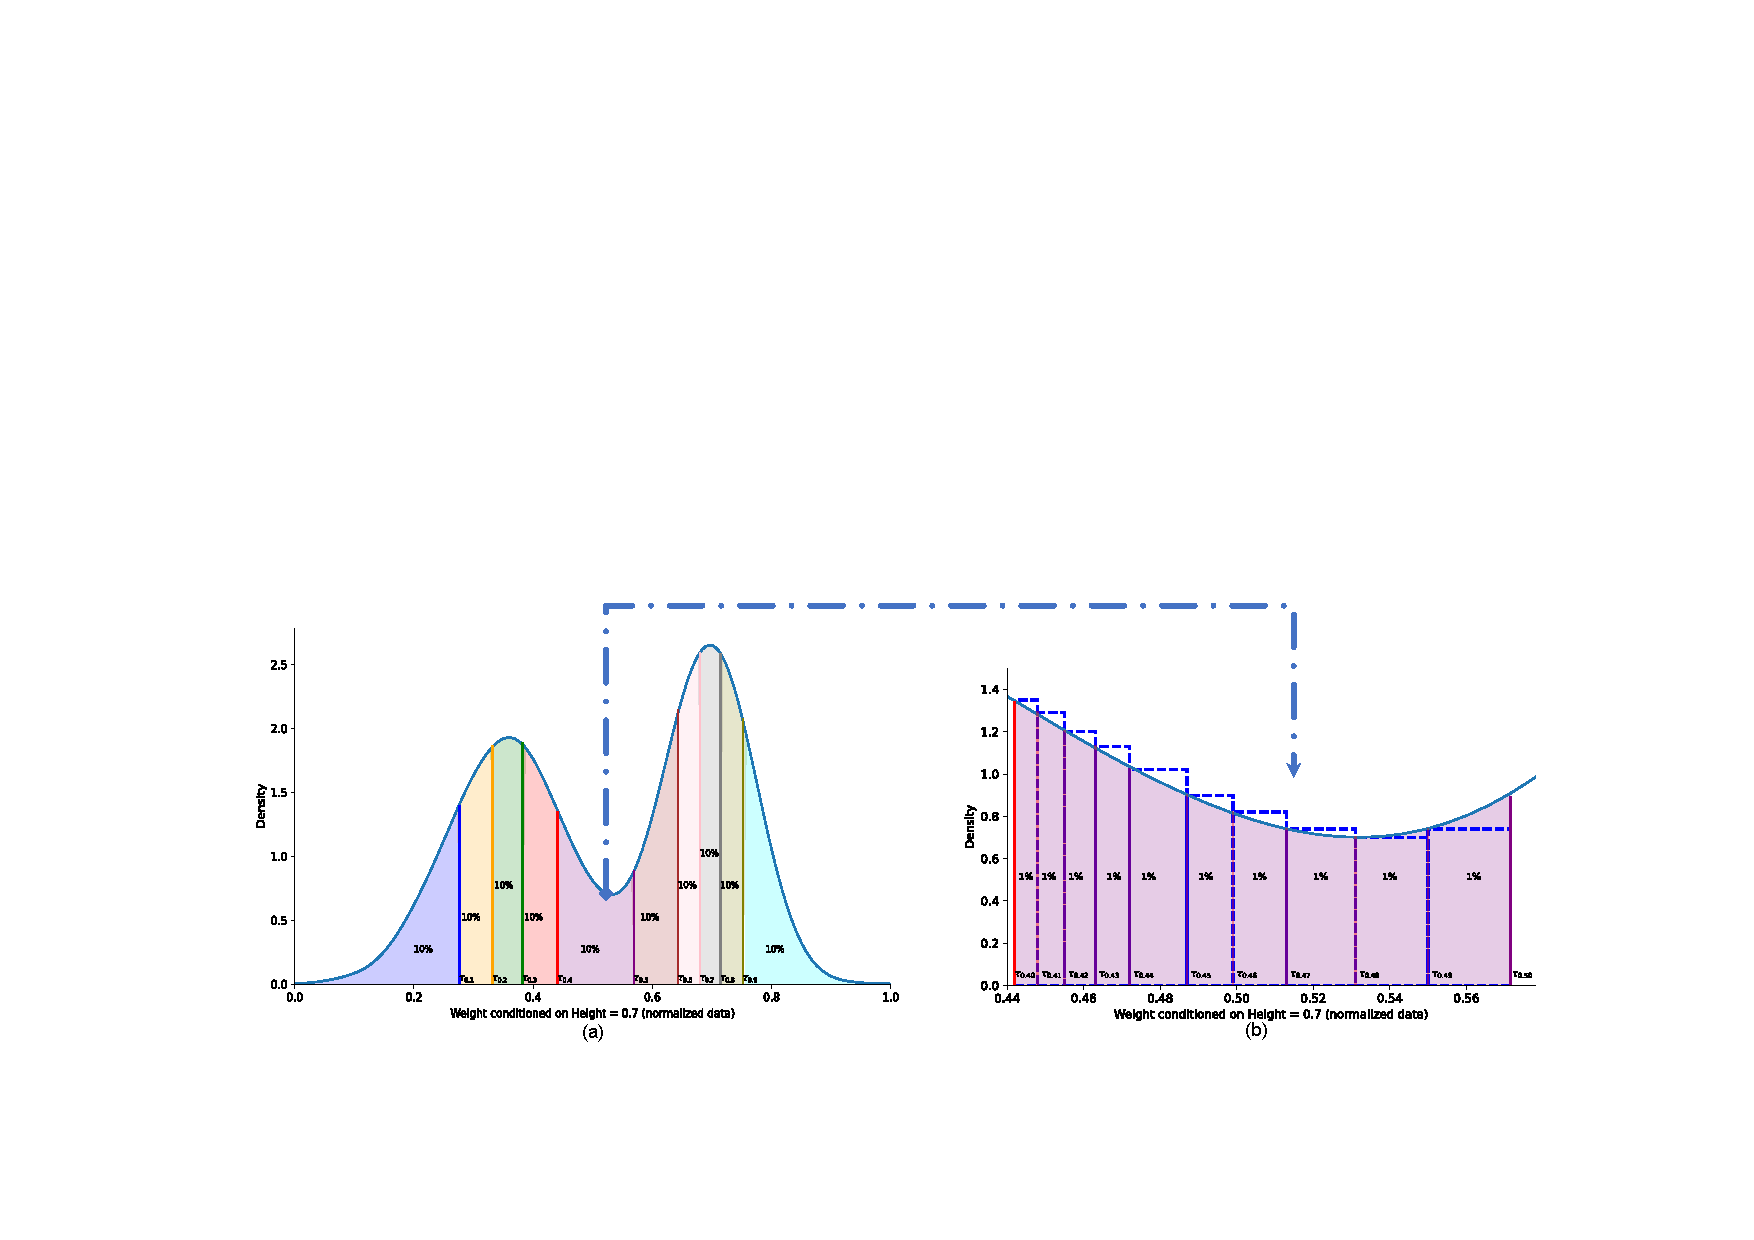
\includegraphics[width=12cm]{images/Pic_quantile_example.pdf}
	\caption{(a) Lượng phân vị có điều kiện ước tính $\{Q_{0.1}, Q_{0.2}, \ldots ,Q_{0.9}\}$ cho một đặc trưng hành vi dựa trên các đặc điểm ngữ cảnh. (b) Phóng to khu vực giữa $Q_{0.40}$ và $Q_{0.50}$, chúng tôi thấy rằng các phân vị có nhiều khả năng đủ chi tiết hơn các phân vị trong (a).}\label{fig:quantile}
\end{figure}

Đây là lúc các khu rừng hồi quy phân vị phát huy tác dụng: được cung cấp đủ dữ liệu huấn luyện, chúng tìm hiểu chính xác hàm phân phối tích lũy có điều kiện, hàm này có thể được truy vấn ở dạng nghịch đảo, tức là thông qua các phân vị có điều kiện. Khi truy vấn một khu rừng hồi quy phân vị, điều này có thể được thực hiện ở các mức độ chi tiết khác nhau. Ví dụ: Hình~\ref{fig:quantile}(a) cho thấy rằng lượng phân vị có điều kiện $\{Q_{0.1}, Q_{0.2}, \ldots ,Q_{0.9}\}$ rất có thể không đủ để mô tả chính xác phân bố có điều kiện vì chúng làm trơn quá mức phân bố cơ bản và do đó không thể nắm bắt chính xác các sắc thái, trong khi Hình~\ref{fig:quantile}(b) cho thấy \emph{percentiles} có điều kiện, tức là, $\{Q_{0.01}, Q_{0.02}, \ldots ,Q_{0.99}\}$ có nhiều khả năng cung cấp đầy đủ chi tiết hơn.

Chúng tôi sử dụng phân vị có điều kiện cho điểm bất thường vì chúng cung cấp mức độ chi tiết cao trong khi không yêu cầu lượng dữ liệu quá lớn để ước tính chính xác.
Là một lợi ích bổ sung, sự khác biệt giữa mỗi phần trăm liên tiếp luôn được đánh giá bằng sự kết hợp có trọng số của số lượng điểm dữ liệu huấn luyện có thể so sánh được, tức là với chi phí làm mịn, chúng tôi không phải chịu ước tính mật độ cục bộ cực kỳ kém ở các khu vực có mật độ thấp.

Để chính thức phát triển điểm bất thường, trước tiên chúng tôi xác định $\tau_i$ là phân vị $i$th, tức là $\tau_i = Q_{i/100}, \forall i \in [0,100]$. Đối với bất kỳ \emph{percentile interval} nào, tức là một khoảng $[\tau_i, \tau_{i+1}]$ được xác định bởi hai phân vị liên tiếp $i$ và $i+1$, theo định nghĩa, chúng ta có định nghĩa rằng nó bao trùm chính xác xác suất $0.01$ (xem Hình~\ref{fig:quantile}(b)). Chúng tôi có thể ước tính mật độ cục bộ của một khoảng phần trăm và sử dụng mật độ đó cho điểm bất thường của mình, nhưng chúng tôi hướng tới điểm số trở nên lớn hơn khi một điểm dữ liệu được coi là bất thường hơn.Để đạt được mục đích này, chúng tôi xác định \emph{độ rộng khoảng phần trăm} $w_i$ là sự khác biệt giữa hai phần trăm liên tiếp $i$ và $i+1$, tức là $\tau_{i+1} - \tau_i$. Như vậy, độ rộng khoảng có thể được coi là 'mật độ nghịch đảo', nghĩa là chiều rộng sẽ tăng khi mật độ cục bộ giảm. Ví dụ, trong Hình~\ref{fig:quantile}(b), chúng ta có $\tau_{46} = 0.5$ và $\tau_{47} = 0.513$, mang lại $w_{46} = 0.013$. Các điểm dữ liệu nằm trong các khoảng phân vị có độ rộng tương đối lớn có nhiều khả năng là các điểm bất thường theo ngữ cảnh hơn, vì chúng nằm trong các khu vực có mật độ thấp của phân bố có điều kiện.

Do đó, ý tưởng cơ bản là xác định điểm bất thường cho đối tượng $\mathbf{x}$ và đặc trưng hành vi $\mathbf{b}^{q}$ là $w(\mathbf{x}\rvert\mathbf{b}^{q})$, tức là độ rộng của khoảng phân vị (được dự đoán bằng QRF) trong đó giá trị hành vi của điểm dữ liệu rơi vào. Tuy nhiên, chúng ta cần xem xét một trường hợp đặc biệt: giá trị đặc trưng hành vi thực tế $b^{q}$ có thể nhỏ hơn phân vị có điều kiện ước tính nhỏ nhất, tức là $\tau_{0}^{q}$ hoặc lớn hơn phân vị có điều kiện ước tính lớn nhất, tức là $\tau_{100}^{q}$. Nghĩa là, giá trị thực tế có thể không rơi vào bất kỳ khoảng phân vị có điều kiện ước tính nào. Để giải quyết vấn đề này, chúng tôi ngoại suy ngoài $\tau_{0}^{q}$ và $\tau_{100}^{q}$, dẫn đến điểm bất thường trung gian

\begin{equation}
\centering
is(\mathbf{x}\rvert\mathbf{b}^{q})=\left\{
\begin{aligned}\left(1+\frac{\tau_{0}^{q}-b^{q}}{\tau_{75}^{q}-\tau_{25}^{q}}\right)\mathrm{max}(w(\mathbf{x}\rvert\mathbf{b}^{q}))&, \text{ if } b^{q} < \tau_{0}^{q} ; \\
\left(1+\frac{b^{q}-\tau_{100}^{q}}{\tau_{75}^{q}-\tau_{25}^{q}}\right)\mathrm{max}(w(\mathbf{x}\rvert\mathbf{b}^{q}))&, \text{ if }  b^{q} > \tau_{100}^{q}, \\
w(\mathbf{x}\rvert\mathbf{b}^{q})&, \text{ otherwise},\\
\end{aligned}
\right.
\label{eq4}
\end{equation}
trong đó $\mathrm{max}(w(\mathbf{x}\rvert\mathbf{b}^{q}))$ biểu thị độ rộng khoảng tối đa của tất cả các khoảng phân vị có điều kiện cho đặc trưng hành vi $\textbf{b}^{q}$.

Thật không may, việc sử dụng trực tiếp Equation~(\ref{eq4}) làm điểm bất thường một phần sẽ khiến cách tiếp cận của chúng ta dễ dẫn đến cái gọi là \textbf{hiệu ứng chính tả}: việc tính tổng điểm từng phần như vậy cho một điểm dữ liệu mà \emph{mạnh mẽ} sai lệch chỉ trong một đặc trưng hành vi \emph{vài} sẽ dẫn đến điểm bất thường lớn hơn dữ liệu dị thường điểm sai lệch vừa phải trong các đặc trưng hành vi của \emph{nhiều}. Kết quả là, những điểm dữ liệu có ít độ lệch lớn sẽ “quyết định” điểm cao nhất; điều này là không mong muốn.

Để tránh hiệu ứng độc tài, chúng tôi cắt bớt điểm bất thường từng phần đến mức tối đa được xác định trước và đi đến điểm bất thường từng phần cuối cùng như

\begin{equation}
\centering
s(\mathbf{x}\rvert\mathbf{b}^{q})=\left\{
\begin{aligned} \frac{\eta}{100} &, \text{ if } is(\mathbf{x}\rvert\mathbf{b}^{q}) > \frac{\eta}{100}; \\
is(\mathbf{x}\rvert\mathbf{b}^{q})&, \text{ otherwise}, \\
\end{aligned}
\right.
\label{eq6}
\end{equation}trong đó $\eta$ là siêu tham số. Cơ sở lý luận cho $\eta$ như sau: nếu phân bố có điều kiện được phân bố đồng đều và đặc trưng hành vi có phạm vi $[0,1]$ thì chiều rộng dự kiến ​​của bất kỳ chiều rộng khoảng phân vị nào là $0.01$ và $\eta$ có thể được hiểu là số lượng tối đa của \emph{độ rộng khoảng phân vị dự kiến}. Trong các thử nghiệm, chúng tôi sử dụng $\eta = 10$ vì hiệu suất thực nghiệm mạnh mẽ của nó (cũng được thể hiện trong nghiên cứu cắt bỏ ở Phụ lục ~ \ref{Appendix:Ablation}).

Bằng cách chia tỷ lệ các đặc trưng hành vi thành $[0,1]$ trước khi phát hiện sự bất thường, ví dụ: sử dụng chuẩn hóa tối thiểu-tối đa, phần trăm có điều kiện ước tính cũng phải nằm trong khoảng này và do đó, độ rộng khoảng thu được cho các đặc trưng hành vi riêng lẻ sẽ có thể so sánh được. Đổi lại, điều này ngụ ý rằng chúng có thể được tính tổng để có được điểm bất thường cuối cùng cho một điểm dữ liệu (Thuật toán~\ref{algo:QCAD}, Dòng 9).

\subsection{Giải thích sự bất thường bằng biểu đồ beanplot bất thường}
\label{qcad:ae}

Trong giai đoạn thứ ba, chúng tôi đưa ra lời giải thích cho những điểm bất thường được báo cáo. Từ định nghĩa về điểm bất thường của chúng tôi, rõ ràng đó là \textit{có thể phân bổ}: điểm tổng thể có thể được phân tách thành một phần điểm cho các đặc trưng hành vi riêng lẻ.

Đối với mỗi điểm bất thường được xác định $\mathbf{a}$, chúng tôi báo cáo các lân cận theo ngữ cảnh của nó là $R(\mathbf{a})$ và điểm bất thường cuối cùng được tính toán trên Dòng~9 của Thuật toán~\ref{algo:QCAD}. Hơn nữa, chúng tôi báo cáo điểm bất thường một phần tương ứng với các đặc trưng hành vi, tức là chúng tôi báo cáo $s(\mathbf{x}\rvert\mathbf{b}^{q})$ cho tất cả $q$, được xếp hạng từ cao nhất đến thấp nhất để cho biết đặc trưng hành vi nào có sự bất thường sai lệch nhiều nhất.

\begin{figure}[tb]
	\centering
	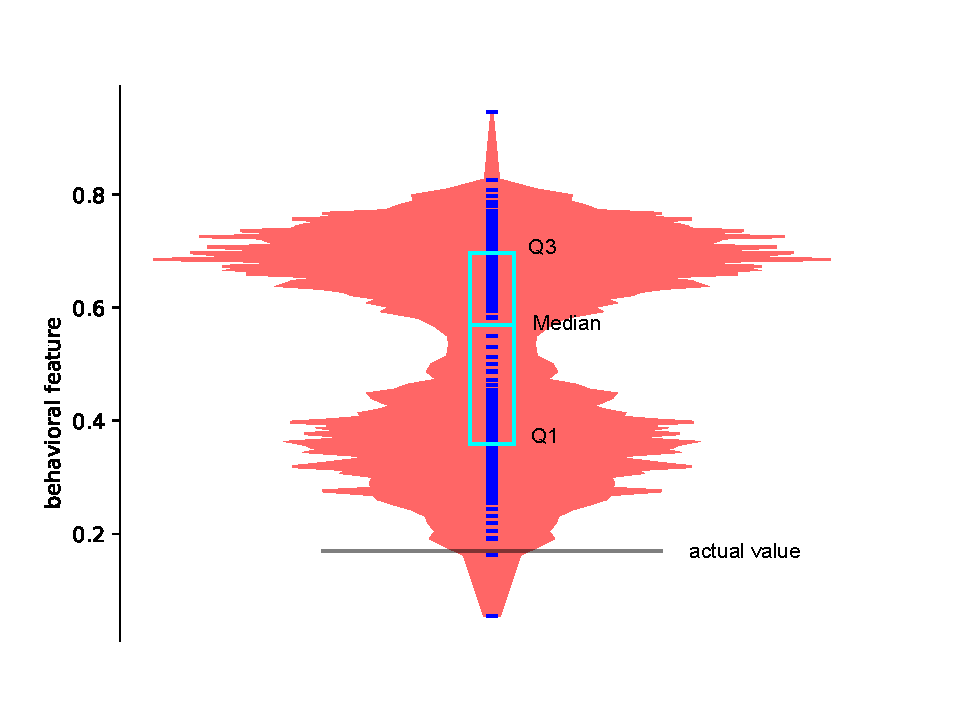
\includegraphics[width=9cm]{images/Pic_beanplot.pdf}
	\caption{Biểu đồ bất thường cung cấp cái nhìn sâu sắc về những gì rừng hồi quy phân vị đã học được đối với một điểm dữ liệu và đặc trưng hành vi cụ thể cũng như lý do tại sao điểm dữ liệu đó (không) được coi là điểm bất thường. Các đường ngắn màu xanh lam biểu thị phần trăm có điều kiện $\tau_0,\tau_1,\ldots,\tau_{100}$ mà QRF đã học được (từ trên xuống dưới), đối với điểm dữ liệu và đặc trưng hành vi nhất định. Như trong biểu đồ hình hộp, hộp (màu lục lam) biểu thị tứ phân vị thứ nhất ($\tau_{25}$), trung vị ($\tau_{50}$) và tứ phân vị thứ ba ($\tau_{75}$). Vùng màu đỏ rộng hơn biểu thị mật độ xác suất được ước tính dựa trên phân vị có điều kiện. Cuối cùng, đường màu đen biểu thị giá trị thực tế mà điểm dữ liệu có.}\label{fig:beanplot}
\end{figure}

Vì trực quan hóa thường giúp nhanh chóng cung cấp thông tin chi tiết có giá trị nên chúng tôi đề xuất \emph{beanplot bất thường}, một biến thể của Beanplot của \cite{kampstra2008beanplot}. Hình~\ref{fig:beanplot} hiển thị một ví dụ, mô tả trực quan các phần trăm có điều kiện đã học, độ rộng khoảng của chúng và mật độ xác suất có thể được ước tính từ những phần trăm đó, tất cả đều dành cho một điểm dữ liệu cụ thể và đặc trưng hành vi. (Hãy nhớ rằng rừng hồi quy phân vị được học trên nhóm tham chiếu của một điểm dữ liệu, do đó biểu đồ beanplot bất thường cho mỗi điểm dữ liệu có thể khác nhau.)Bằng cách đưa giá trị thực tế của điểm dữ liệu vào biểu đồ Beanplot (dưới dạng một đường màu đen nằm ngang), nhà phân tích có thể dễ dàng thấy giá trị đặc trưng hành vi của nó được định vị như thế nào so với giá trị của nhóm tham chiếu và tại sao cũng như ở mức độ nào nó đóng góp vào sự bất thường của nó.

\section{Thí nghiệm}
\label{sec:experiments}

Để chứng minh tính hiệu quả của phương pháp tiếp cận tổng thể và phương pháp QCAD được đề xuất, chúng tôi tiến hành thử nghiệm trên nhiều bộ dữ liệu tổng hợp và thực tế. Trước tiên, chúng tôi sẽ giải thích các lựa chọn liên quan đến bộ dữ liệu, thuật toán cơ bản và tiêu chí đánh giá, sau đó chúng tôi trình bày cả kết quả định lượng và nghiên cứu điển hình để điều tra khả năng diễn giải và tiện ích thực tế.

Ngoài ra, chúng tôi chứng minh tính mạnh mẽ của QCAD liên quan đến "số lượng siêu tham số lân cận gần nhất bằng phương pháp phân tích độ nhạy và tiến hành một số nghiên cứu cắt bỏ để điều tra tác động của siêu tham số". Vì lý do không gian và sự ngắn gọn, việc phân tích độ nhạy và
nghiên cứu cắt bỏ được đưa ra trong Phụ lục~\ref{Appendix:Sensitivity} và~\ref{Appendix:Ablation}.

\subsection{Dữ liệu}
\label{subsec:datasets}

Việc đánh giá các thuật toán phát hiện bất thường không được giám sát là một thách thức do thiếu dữ liệu điểm chuẩn được thống nhất chung và các bộ dữ liệu phân loại lấy mẫu xuống đã bị chỉ trích vì sự thay đổi về bản chất của các ngoại lệ thu được \citep{farber2010using,campos2016evaluation}.

Khi đánh giá các thuật toán phát hiện bất thường theo ngữ cảnh \emph{không giám sát}, vấn đề này càng trở nên phức tạp hơn do yêu cầu phải có cả các đặc trưng ngữ cảnh và hành vi, đồng thời---quan trọng hơn---xử lý các tính năng đó một cách khác nhau \citep{liang2016robust}. Do đó, một cách tiếp cận được chấp nhận rộng rãi là đưa các điểm bất thường theo ngữ cảnh vào các tập dữ liệu hiện có một cách giả tạo bằng cách sử dụng sơ đồ nhiễu loạn.

\subsubsection{Tiền xử lý dữ liệu}
\label{prelim:gower}

Để làm cho các bộ dữ liệu phù hợp với tất cả các phương pháp phát hiện điểm bất thường, chúng ta cần xử lý trước chúng trước khi đưa vào các điểm bất thường theo ngữ cảnh. Đầu tiên, chúng tôi tận dụng Mã hóa nhãn \citep{seger2018investigation} để chuyển đổi các đặc điểm ngữ cảnh phân loại thành dạng số. Thứ hai, chúng tôi sử dụng chuẩn hóa Min-Max để mở rộng tất cả các đặc trưng hành vi thành $[0,1]$. Chuẩn hóa Min-Max được sử dụng thường xuyên trong nhiều hoạt động phát hiện bất thường và thường cải thiện hiệu suất \citep{kandanaarachchi2020normalization}.\textbf{Khoảng cách của Gower} Để có thể tính toán độ tương tự giữa hai điểm dữ liệu chứa cả đặc điểm phân loại và số, chúng ta có thể sử dụng khoảng cách \citep{gower1971general} của Gower. Cụ thể, khoảng cách của Gower giữa các điểm dữ liệu $\mathbf{c}_{i} = (c_{i}^{1},...,c_{i}^{p},...c_{i}^{P})$ và $\mathbf{c}_{j} = (c_{j}^{1},...,c_{j}^{p},...c_{j}^{P})$ được xác định là $1- \frac{1}{P}\sum_{p=1}^{P}ps_{ij}^{p}$, trong đó $ps_{ij}^{p}$ thể hiện sự tương đồng một phần giữa các phiên bản dữ liệu $\mathbf{c}_{i}$ và $\mathbf{c}_{j}$ trong chiều thứ $p$. Đối với đối tượng số, $ps_{ij}^{p} = 1- \frac{\abs{c_{i}^{p}-c_{j}^{p}}}{\mathrm{max}(\mathbf{c}^p)-\mathrm{min}(\mathbf{c}^p)}$, với $\mathrm{max}(\mathbf{c}^p)$ và $\mathrm{min}(\mathbf{c}^p)$ lần lượt biểu thị giá trị tối đa và tối thiểu của tất cả các điểm dữ liệu cho đối tượng địa lý $p$-th. Đối với tính năng phân loại, $ps_{ij}^{p} = \mathbb{I}(c_{i}^p-c_{j}^p$), trong đó $\mathbb{I}(\cdot)$ đại diện cho chức năng chỉ báo. Do đó, khoảng cách của Gower giữa hai điểm dữ liệu luôn nằm trong $[0,1]$, với giá trị thấp hơn biểu thị mức độ tương tự lớn hơn.

\subsubsection{Lược đồ nhiễu loạn cho việc tiêm ngoại lệ}

\cite{song2007conditional} đã đề xuất một sơ đồ nhiễu loạn để đưa các điểm bất thường theo ngữ cảnh vào các tập dữ liệu không có điểm bất thường trên cơ sở thực tế, đã trở thành một tiêu chuẩn thực tế để đánh giá khả năng phát hiện điểm bất thường theo ngữ cảnh~\citep{song2007conditional, liang2016robust, zheng2017contextual, calikus2021wisdom}.



Tuy nhiên, sơ đồ nhiễu loạn này cũng bị chỉ trích vì hai lý do~\citep{song2007conditional,kuo2018detecting}.
Đầu tiên, các đối tượng thu được bằng cách hoán đổi các giá trị đặc trưng vẫn có khả năng là bình thường về mặt ngữ cảnh. Thứ hai, một số loại dị thường rất phổ biến không thể được giải quyết thông qua sơ đồ nhiễu loạn này. Ví dụ: người ta không thể thu được các giá trị cực trị bằng cách hoán đổi các giá trị đặc trưng trong một tập dữ liệu sạch, trong khi hầu hết các phương pháp phát hiện bất thường đều cho rằng tập dữ liệu huấn luyện không bị nhiễm bẩn. Để tránh những vấn đề này, \cite{kuo2018detecting} đã giới thiệu một sơ đồ nhiễu loạn khác để tạo ra các dị thường. Chúng tôi phát triển một sơ đồ nhiễu loạn mới bằng cách cải tiến sơ đồ này như sau.Với tập dữ liệu $\mathbf{X}$ chứa các phiên bản dữ liệu $N$ với bộ đặc trưng ngữ cảnh $\mathbf{C} = \{\mathbf{c}^{1},...,\mathbf{c}^{P}\}$ và bộ đặc trưng hành vi $\mathbf{B} = \{\mathbf{b}^{1},...,\mathbf{b}^{Q}\}$, trước tiên chúng tôi sử dụng chuẩn hóa Min-Max để chia tỷ lệ các đặc trưng hành vi của tất cả các đối tượng thành $[0,1]$ (giữ nguyên các đặc trưng ngữ cảnh), dẫn đến một tập dữ liệu mới $\Tilde{\mathbf{X}}$. Thứ hai, để đưa các dị thường $m$ vào $\Tilde{\mathbf{X}}$, với $0<m \ll N$, chúng tôi chọn ngẫu nhiên các đối tượng $m$ $\mathbf{x}_{1},\ldots,\mathbf{x}_{m}$ một cách thống nhất từ ​​$\Tilde{\mathbf{X}}$. Đối với mỗi $\mathbf{x} =(\mathbf{c},\mathbf{b})$ trong $\Tilde{\mathbf{X}}$, $\mathbf{c}$ biểu thị các giá trị đặc trưng ngữ cảnh và $\mathbf{b}$ biểu thị các giá trị đặc trưng hành vi. Thứ ba, đối với đối tượng được chọn $\mathbf{x}_{i} = (\mathbf{c}_{i}, \mathbf{b}_{i})= (c^{1}_{i},...,c^{p}_{i},...,c^{P}_{i},b^{1}_{i},...,b^{q}_{i},...,b^{Q}_{i})$ và đặc trưng hành vi $\mathbf{b}^{q}$, chúng tôi lấy mẫu một số ngẫu nhiên thống nhất từ ​​$[-0.5,-0.1] \bigcup [0.1,0.5]$, sau đó thêm số ngẫu nhiên này vào giá trị đặc trưng hành vi của $\mathbf{x}_{i}$, cụ thể là $b^{q}_{i}$, tạo ra $\hat{b}^{q}_{i}$. Theo cách tương tự, chúng tôi lặp lại quy trình này cho từng đặc trưng hành vi, tạo ra $(\hat{b}^{1}_{i},...,\hat{b}^{Q}_{i})$ hoặc $\hat{\mathbf{b}}_{i}$. Theo đó, chúng ta tạo ra một đối tượng mới
$\tilde{\mathbf{x}} = (\mathbf{c}, \hat{\mathbf{b}})$ là sự bất thường theo ngữ cảnh. Thứ tư, chúng tôi lặp lại bước thứ ba cho từng đối tượng được chọn, dẫn đến các đối tượng bị nhiễu loạn $m$.
Thứ năm và cuối cùng, chúng tôi thay thế các đối tượng đã chọn trong tập dữ liệu gốc bằng các đối tượng nhiễu loạn tương ứng của chúng. Để cho phép chèn các giá trị cực trị, chúng tôi cố tình không cắt bớt các giá trị bên ngoài $[0,1]$ sau khi thêm một số ngẫu nhiên vào từng đặc trưng hành vi.

Sơ đồ nhiễu loạn của chúng tôi có những ưu điểm sau. Khi so sánh với sơ đồ nhiễu loạn hoán đổi do \cite{song2007conditional} đề xuất, các đối tượng thu được từ sơ đồ nhiễu loạn của chúng tôi rất khó có thể duy trì trạng thái bình thường theo ngữ cảnh. Ngoài ra, sơ đồ nhiễu loạn của chúng ta có thể---nhưng không phải lúc nào cũng---dẫn đến các giá trị cực trị. Lưu ý rằng chúng tôi không tuân thủ nghiêm ngặt sơ đồ nhiễu loạn do \cite{kuo2018detecting} đề xuất vì phương pháp của họ chỉ thêm một số không âm vào các đặc trưng hành vi. Một mặt, đôi khi số không âm này bằng 0, dẫn đến việc tiêm vào một vật thể bình thường là ``dị thường'. Mặt khác, đôi khi con số không âm này rất lớn, khiến đối tượng được tiêm (cũng) dễ bị phát hiện. Sơ đồ nhiễu loạn của chúng tôi tránh được những vấn đề này bằng cách trước tiên bình thường hóa các giá trị đặc trưng hành vi, sau đó thiết lập các giới hạn trên và dưới hợp lý hơn cho nhiễu loạn.

\subsubsection{Bộ dữ liệu}

Để đánh giá và so sánh phương pháp của chúng tôi trên nhiều loại bộ dữ liệu khác nhau, chúng tôi tạo bộ dữ liệu tổng hợp $10$ và chọn bộ dữ liệu trong thế giới thực $20$; các thuộc tính của chúng được tóm tắt lần lượt trong các Bảng~\ref{tab:data_summary1} và \ref{tab:data_summary2}.\begin{table}[!htbp]
	\caption{Tóm tắt các bộ dữ liệu tổng hợp. $\#Num, \#Cat, \#\mathbf{C}$ và $\#\mathbf{B}$ lần lượt biểu thị số lượng đối tượng số, số lượng đối tượng phân loại/danh nghĩa, số lượng đối tượng theo ngữ cảnh và số lượng đối tượng hành vi. Tất cả các đặc trưng hành vi đều là số, các đặc điểm ngữ cảnh có thể được trộn lẫn.}
	\centering
	\begin{tabular}{cccccc}
		\toprule
		Bộ dữ liệu &Sơ đồ & \#Num & \#Cat & \#$\mathbf{C}$ & \#$\mathbf{B}$ \\
		\midrule
		Syn1 & S1 & 8 & 2 & 5 & 5 \\
		\midrule
		Syn2 & S2 & 8 & 2 & 5 & 5 \\
		\midrule
		Syn3 & S3 & 8 & 2 & 5 & 5 \\
		\midrule
		Syn4 & S4 & 8 & 2 & 5 & 5 \\
		\midrule
		Syn5 & S5 & 8 & 2 & 5 & 5 \\
		\midrule
		Syn6 & S1 & 19 & 6 & 20 & 5 \\
		\midrule
		Syn7 & S2 & 19 & 6 & 20 & 5 \\
		\midrule
		Syn8 & S3 & 19 & 6 & 20 & 5 \\
		\midrule
		Syn9 & S4 & 19 & 6 & 20 & 5 \\
		\midrule
		Syn10 & S5 & 19 & 6 & 20 & 5 \\
		\bottomrule
	\end{tabular}
	\label{tab:data_summary1}
\end{table}

Đầu tiên chúng ta thảo luận về dữ liệu tổng hợp. Để có thể tạo ra dữ liệu với nhiều dạng và mức độ phụ thuộc khác nhau giữa các đặc trưng hành vi và ngữ cảnh, chúng tôi đề xuất các sơ đồ tạo sau. Đối với $q \in \{1,...,Q\}$, chúng tôi có
\begin{itemize}
    \item[(S1)] $\mathbf{b}^{q} = \sum_{p=1}^{Q}\left(\alpha_{qp}\cdot\mathbf{c}^{p}\right)+\boldsymbol{\epsilon}$;
    \item[(S2)] $\mathbf{b}^{q} = \sum_{p=1}^{Q}\left(\alpha_{qp}\cdot(\mathbf{c}^{p})^{3}\right)+\boldsymbol{\epsilon}$,
    \item[(S3)] $\mathbf{b}^{q} = \sum_{p=1}^{Q}\left(\alpha_{qp}\cdot\mathrm{sin}(\mathbf{c}^{p})\right)+\boldsymbol{\epsilon}$,
    \item[(S4)] $\mathbf{b}^{q} = \sum_{p=1}^{Q}\left(\alpha_{qp}\cdot\mathrm{log}(\mathbf{1}+\vert\mathbf{c}^{p}\vert)\right)+\boldsymbol{\epsilon}$,
    \item[(S5)] $\mathbf{b}^{q} = \sum_{p=1}^{Q}\left(\alpha_{qp}\cdot\mathbf{c}^{p}+\beta_{qp}\cdot(\mathbf{c}^{p})^{3}+\gamma_{qp}\cdot\mathrm{sin}(\mathbf{c}^{p})+\delta_{qp}\cdot\mathrm{log}(\mathbf{1}+\vert\mathbf{c}^{p}\vert)\right)+\boldsymbol{\epsilon}$,
\end{itemize}
trong đó $\alpha_{qp}, \beta_{qp},\gamma_{qp}, \delta_{qp} \stackrel{i.i.d.}{\sim} \mathcal{U}(0,1)$ và được thay thế bằng 0 với xác suất là $1/3$. Hơn nữa, $\boldsymbol{\epsilon} = (\epsilon_{1},...,\epsilon_{n},...,\epsilon_{N})^{T}$, với $\epsilon_{n} \stackrel{i.i.d.}{\sim} \mathcal{U}(0,0.05)$.Ngoài ra, đối với $p \in \{1,...,P\}$, $\mathbf{c}^{p}$ được tạo từ mô hình hỗn hợp Gaussian với năm cụm. Nếu là số, thì mỗi tâm Gaussian được lấy mẫu ngẫu nhiên một cách thống nhất từ ​​$[0,1]$ và phần tử đường chéo của ma trận hiệp phương sai được cố định tại $1/4$ của khoảng cách trung bình theo cặp giữa các tâm trong mỗi đặc trưng hành vi. Mặt khác, các trọng tâm được lấy mẫu ngẫu nhiên một cách thống nhất từ ​​$\{0,1,...,10\}$ với cùng cài đặt hiệp phương sai. Hơn nữa, mọi số được tạo đều được làm tròn thành số nguyên để đảm bảo rằng nó mang tính phân loại. Trên cơ sở này, chúng tôi tạo ra một bộ sưu tập lớn các bộ dữ liệu tổng hợp bằng cách thay đổi sơ đồ tạo cũng như số lượng đặc trưng ngữ cảnh và đặc trưng hành vi. Cỡ mẫu luôn được đặt thành $2000$ và tốc độ dị thường được đưa vào được cố định ở $2.5\%$. Xem Bảng~\ref{tab:data_summary1} để biết tổng quan.

\begin{table}[!htbp]
	\caption{Tóm tắt các bộ dữ liệu trong thế giới thực. $\#Num, \#Cat, \#\mathbf{C}$ và $\#\mathbf{B}$ lần lượt biểu thị số lượng đối tượng số, số lượng đối tượng phân loại/danh nghĩa, số lượng đối tượng theo ngữ cảnh và số lượng đối tượng hành vi. Tất cả các đặc trưng hành vi đều là số, các đặc điểm ngữ cảnh có thể được trộn lẫn.}
	\centering
	\begin{tabular}{cccccccc}
		\toprule
		Bộ dữ liệu & \#Num & \#Cat & \#Samples & \#Abất thường (Tỷ lệ) & \#$\mathbf{C}$ & \#$\mathbf{B}$ \\
		\midrule
		Bào ngư & 8 & 1 & 4177 & 100 (2.4\%) & 4 & 5 \\
		AirFoil & 6 & 0 & 1503 & 70 (4.7\%) & 5 & 1 \\
		BodyFat & 15 & 0 & 252 & 20 (7.9\%) & 13 & 2 \\
		Boston & 12 & 2 & 506 & 40 (7.9\%) & 13 & 1 \\
		Bê tông & 9 & 0 & 1030 & 50 (4.8\%) & 8 & 1 \\
		ElNino & 3 & 8 & 20000 & 200 (1\%) & 6 & 5 \\
		Năng lượng & 10 & 0 & 768 & 50 (6.5\%) & 8 & 2 \\
		Trọng lượng cá & 6 & 1 & 157 & 15 (9.5\%) & 6 & 1 \\
		Cháy rừng & 11 & 2 & 517 & 50 (9.7\%) & 4 & 9 \\
		GasEmission & 11 & 0 & 7384 & 100 (1.4\%) & 8 & 3 \\
		HeartFailure & 7 & 5 & 299 & 30 (10\%) & 6 & 6 \\
		Viêm gan & 11 & 2 & 615 & 30 (4.9\%) & 3 & 10 \\
		Bệnh nhân gan & 9 & 2 & 579 & 30 (5.2\%) & 3 & 8 \\
		Bảo trì & 18 & 0 & 11934 & 100 (0.8\%) & 15 & 3 \\
		Parkinson & 21 & 1 & 5875 & 100 (1.7\%) & 20 & 2 \\
        PowerPlant & 5 & 0 & 9568 & 100 (1\%) & 4 & 1 \\
		QSRanking & 12 & 1 & 475 & 40 (8.4\%) & 7 & 6 \\
		SynMachine & 5 & 0 & 557 & 50 (8.9\%) & 4 & 1 \\
		Độc tính & 7 & 0 & 908 & 50 (5.5\%) & 6 & 1 \\
		Du thuyền & 7 & 0 & 308 & 30 (9.7\%) & 6 & 1 \\
		\bottomrule
	\end{tabular}
	\label{tab:data_summary2}
\end{table}Tiếp theo, chúng tôi sử dụng sơ đồ nhiễu loạn được đề cập ở trên để đưa các điểm bất thường theo ngữ cảnh vào bộ dữ liệu trong thế giới thực $20$. Chúng tôi sử dụng các bộ dữ liệu này vì chúng đại diện cho các lĩnh vực ứng dụng tiềm năng trong khung QCAD của chúng tôi. Nghĩa là, chúng bắt nguồn từ khoa học đời sống \& chăm sóc sức khỏe (ví dụ: Bodyfat, Suy tim, Bệnh nhân sông Ấn Độ, Viêm gan, Giám sát từ xa bệnh Parkinson, Bào ngư, Trọng lượng cá, Độc tính cá QSAR), khoa học xã hội (ví dụ: Giá nhà ở Boston, Xếp hạng trường đại học), khu vực bảo vệ môi trường (ví dụ: El Nino, Cháy rừng) và kỹ thuật (ví dụ: Phát thải tuabin khí CO và NOx, Thủy động lực học du thuyền, Điều kiện Dựa trên việc bảo trì các nhà máy động lực hải quân, máy đồng bộ, độ ồn của cánh máy bay, cường độ nén bê tông, nhà máy điện chu trình hỗn hợp). Bản tóm tắt được đưa ra trong Bảng \ref{tab:data_summary2}; mỗi tập dữ liệu được mô tả chi tiết hơn trong Phụ lục~\ref{Appendix:Data}.

\subsection{Thuật toán cơ bản và cách triển khai}
\label{subsec:baselines}

Về mặt thực nghiệm, chúng tôi so sánh phương pháp của mình với các thuật toán tiên tiến, bao gồm các phương pháp phát hiện điểm bất thường truyền thống (dựa trên khoảng cách, dựa trên mật độ, dựa trên sự phụ thuộc, v.v.) và các phương pháp phát hiện điểm bất thường theo ngữ cảnh. Để so sánh công bằng, chúng tôi chọn các công cụ phát hiện điểm bất thường sau đây, tất cả đều trả về điểm bất thường---chứ không phải kết quả nhị phân---cho mỗi phiên bản dữ liệu.
\begin{itemize}
    \item Phương pháp dự đoán cục bộ để phát hiện bất thường (LoPAD) của \cite{lu2020lopad}, đây là công cụ phát hiện bất thường truyền thống dựa trên sự phụ thuộc tiên tiến nhất;
    \item Phát hiện ngoại lệ có điều kiện (CAD) của \cite{song2007conditional}, đây là công cụ phát hiện bất thường đầu tiên chuyên dụng để xác định các bất thường theo ngữ cảnh;
    \item Phát hiện ngoại lệ theo ngữ cảnh mạnh mẽ (ROCOD) của \cite{liang2016robust}, đây là công cụ phát hiện bất thường theo ngữ cảnh tiên tiến nhất;
    \item Rừng cách ly (IForest) của \cite{liu2008isolation}, một trong những máy dò dị thường truyền thống dựa trên sự cách ly tiên tiến nhất;
    \item Hệ số ngoại lệ cục bộ (LOF) của \cite{breunig2000lof}, một trong những máy dò dị thường truyền thống dựa trên mật độ tiên tiến nhất;
    \item Máy dò dị thường $k$-NN của \cite{angiulli2002fast}, một trong những máy dò dị thường truyền thống dựa trên khoảng cách tiên tiến nhất;
    \item Máy dò dị thường sử dụng không gian con song song trục (SOD) của \cite{kriegel2009outlier}, một trong những máy dò dị thường truyền thống dựa trên không gian con tiên tiến nhất; và
    \item Điểm ngoại lệ dựa trên biểu đồ (HBOS) của \cite{goldstein2012histogram}, một trong những công cụ phát hiện bất thường truyền thống dựa trên biểu đồ hiện đại.
\end{itemize}Chúng tôi đã triển khai và chạy tất cả các thuật toán trong Python $3.8$ trên máy tính có CPU lõi 8 chip Apple M1 và bộ nhớ hợp nhất 8GB. Đối với các thuật toán cổ điển như IForest, LOF, $k$-NN, SOD và HBOS, chúng tôi sử dụng các triển khai có sẵn công khai của chúng trong PyOD \citep{zhao2019pyod} với cài đặt mặc định của chúng. Thật không may, đối với LoPAD, CAD và ROCOD không có triển khai nào được công bố rộng rãi. Đối với LoPAD, trước tiên chúng tôi sử dụng gói `bnlearn' \citep{scutari2019package} trong R để tìm Markov Chăn của từng tập dữ liệu dựa trên Fast-IAMB \citep{yaramakala2005speculative}. Tiếp theo, chúng tôi triển khai thuật toán LoPAD bằng Python bằng cách sử dụng CART \citep{breiman2017classification} làm mô hình dự đoán với kích thước đóng bao $200$. Đối với CAD, chúng tôi triển khai thuật toán CAD-GMM-Full theo khuyến nghị của \cite{song2007conditional}, với cài đặt mặc định ngoại trừ tham số `số thành phần Gaussian'; nếu tham số này được đặt thành 30 mặc định, thì sẽ mất hơn một tháng để hoàn thành tất cả các thử nghiệm trên máy tính của chúng tôi. Ngoài ra, các thử nghiệm sơ bộ cho thấy sự khác biệt về kết quả khi tham số này được đặt thành $30$ và $5$ tương ứng là không đáng kể đối với hầu hết các bộ dữ liệu. Do đó, chúng tôi đặt tham số này thành $5$ trong tất cả các thử nghiệm. Chúng tôi đã triển khai ROCOD bằng Python với cài đặt mặc định. Tuy nhiên, một tham số quan trọng, đó là ngưỡng khoảng cách được sử dụng để tìm hàng xóm, không được thảo luận trong \cite{liang2016robust}. Đối với các tập dữ liệu và số liệu khoảng cách khác nhau, thật khó để có được một giá trị tốt nhất cho tham số này và các thử nghiệm sơ bộ cho thấy ROCOD rất nhạy cảm với tham số này. Tuy nhiên, chúng tôi cũng quan sát thấy rằng nó thường đạt được kết quả tương đối tốt khi ngưỡng khoảng cách được sử dụng để tìm hàng xóm được đặt thành $0.9$; do đó, chúng tôi quyết định đặt tham số này thành $0.9$ theo mặc định.

\subsubsection{Cài đặt tham số QCAD}
\label{subsec:ParametersSettings}


Như được tóm tắt trong Bảng \ref{tab:parameters}, thuật toán QCAD cũng yêu cầu thiết lập một số tham số. Đầu tiên, trong khung bất thường theo ngữ cảnh của chúng tôi, chúng tôi cần đặt số lượng lân cận gần nhất ($k$) được sử dụng để tạo nhóm tham chiếu. Thứ hai, khi tạo rừng hồi quy phân vị, chúng ta cần chỉ định các tham số sau: số lượng cây, số lượng đối tượng tối đa được sử dụng để xây dựng cây và số lượng cỡ mẫu tối thiểu để phân chia trong một nút của cây. Thứ ba, chúng ta cần chỉ định số lượng phân vị có điều kiện ($l$) để ước tính cho một đối tượng trong từng đặc trưng hành vi. Cuối cùng, chúng ta cũng cần đặt số lượng tính năng ($h$) được sử dụng để tạo phần giải thích. Chúng tôi thiết lập các thông số này như sau.\begin{table}
  \caption{Tóm tắt các tham số liên quan đến QCAD. Đặc biệt, \textbf{Value} đại diện cho các giá trị mà chúng tôi khuyên bạn nên sử dụng trong thử nghiệm.}
  \label{tab:parameters}
  \centering
  \begin{tabular}{ccc}
    \toprule
    \textbf{Ký hiệu} & \textbf{Ý nghĩa} & \textbf{Giá trị}\\
    \midrule
    $k$ & số hàng xóm gần nhất & $\mathrm{min}(N/2,500)$\\
    $n_q$ & số lượng phân vị có điều kiện cần ước tính & $100$\\
    $n_t$ & số cây được sử dụng để tạo QRF & $100$ hoặc $10$\\
    $n_f$ & số lượng tính năng tối đa được sử dụng để xây dựng cây & $\vert\mathbf{C}\vert$\\
    $n_s$ & số lượng mẫu tối thiểu để phân chia một nút & $10$\\
    $h$ & số tính năng được sử dụng để tạo giải thích & $\mathrm{min}(\vert \mathbf{B} \vert,3)$\\
  \bottomrule
\end{tabular}
\end{table}

\begin{itemize}
\item Số lượng láng giềng gần nhất ($k$): phân tích độ nhạy (xem phụ lục) chỉ ra rằng phương pháp của chúng tôi là chắc chắn đối với tham số này miễn là giá trị của nó không quá nhỏ. Theo mặc định, chúng tôi đặt tham số này thành $\mathrm{min}(N/2,500)$, trong đó $N$ là kích thước mẫu.

\item Số lượng phân vị có điều kiện cần ước tính ($n_q$): về mặt lý thuyết, việc tăng số lượng này sẽ mang lại hiệu suất tốt hơn về mặt độ chính xác, nhưng phải trả giá bằng thời gian chạy lớn hơn. Tuy nhiên, các thử nghiệm sơ bộ cho thấy việc tăng con số này vượt quá $100$ sẽ chỉ mang lại kết quả tốt hơn một chút. Do đó, chúng tôi đặt nó thành $100$ theo mặc định.

\item Số lượng cây được sử dụng để xây dựng rừng hồi quy phân vị ($n_t$): về lý thuyết, số lượng cây lớn hơn sẽ mang lại hiệu suất tốt hơn về mặt độ chính xác, nhưng phải trả giá bằng thời gian chạy lớn hơn. Bằng thực nghiệm, chúng tôi nhận thấy rằng cây 100 thường cho kết quả tốt và việc tăng thêm số lượng cây dẫn đến sự cải thiện không đáng kể. Do hạn chế về thời gian, chúng tôi đặt số này thành 10 trong tất cả các thử nghiệm trong bài viết này.

\item Số lượng đặc điểm tối đa được sử dụng để xây dựng cây trong rừng hồi quy phân vị ($n_f$): \cite{meinshausen2006quantile} đã chứng minh tính ổn định của rừng hồi quy phân vị trên tham số này và đặt tham số này thành $1/3$ của số lượng biến trong thử nghiệm của họ. Tuy nhiên, trong các thử nghiệm của chúng tôi, đôi khi số lượng đặc trưng ngữ cảnh ít hơn 3. Để hiển thị các khu rừng hồi quy phân vị có thể áp dụng trên các tập dữ liệu khác nhau, chúng tôi đặt tham số này thành số lượng của tất cả các biến theo mặc định.

\item Kích thước mẫu tối thiểu cho nút của cây được phân tách ($n_s$): như được chỉ ra trong \cite{meinshausen2006quantile}, các giá trị khác nhau của tham số này dường như không ảnh hưởng nhiều đến kết quả và các thử nghiệm sơ bộ của chúng tôi cũng phù hợp với tuyên bố này. Do đó, chúng tôi đặt số này thành $10$ theo mặc định, cũng như được sử dụng trong \cite{meinshausen2006quantile}.
\item Số lượng tính năng được sử dụng để tạo giải thích ($h$): Tham số này được đặt thành $\mathrm{min}(\vert \mathbf{B} \vert,3)$ theo mặc định. Tuy nhiên, người dùng cuối có thể đặt tham số này theo sở thích của họ miễn là giá trị của nó nằm trong khoảng $0$ và $\vert \mathbf{B} \vert $, trong đó
$\vert \mathbf{B} \vert $ đại diện cho số lượng đặc trưng hành vi.
\end{itemize}Để có thể tái sử dụng, chúng tôi công khai tất cả mã và tập dữ liệu\footnote{https://github.com/ZhongLIFR/QCAD}.

\subsection{Tiêu chí đánh giá}
\label{subsec:metrics}

PRC AUC \citep{liang2016robust,kuo2018detecting}, ROC AUC \citep{micenkova2014learning, micenkova2015learning, pasillas2016unsupervised} và Precision@$n$ \citep{aggarwal2017outlier} được sử dụng rộng rãi để đánh giá và so sánh các phương pháp phát hiện bất thường nhằm tạo ra danh sách đầy đủ các điểm bất thường cho tất cả các quan sát. Chúng được định nghĩa như sau:
\begin{itemize}
    \item Đặc tính hoạt động của máy thu (ROC), có được bằng cách vẽ biểu đồ tỷ lệ dương thực (trục y) so với tỷ lệ dương tính giả (trục x) ở các cài đặt ngưỡng khác nhau. Vùng dưới đường cong này, cụ thể là ROC AUC, là thước đo hiệu suất không xác định ngưỡng được sử dụng rộng rãi trong phát hiện bất thường;
    \item Đường cong thu hồi chính xác (PRC), được tạo bằng cách vẽ đồ thị độ chính xác (trục y) so với thu hồi (trục x) ở các cài đặt ngưỡng khác nhau. Vùng bên dưới đường cong này, cụ thể là PRC AUC, là một thước đo hiệu suất không xác định ngưỡng, được sử dụng rộng rãi khác và còn được gọi là Độ chính xác Trung bình;
    \item Độ chính xác ở $n$, hoặc P@n, được định nghĩa là độ chính xác của các quan sát được xếp hạng trong số $n$ hàng đầu, trong đó $n\in\{1,2,...,N\}$. Trong các thử nghiệm của mình, chúng tôi đặt $n$ thành số lượng điểm bất thường theo ngữ cảnh được đưa vào.
\end{itemize}
Để hoàn thiện: độ chính xác được xác định là $\frac{\#\{\text{Real anomalies}\} \cap \{\text{Reported anomalies}\}}{\#\{\text{Reported anomalies}\}}$, trong khi thu hồi được xác định là $\frac{\#\{\text{Real anomalies}\} \cap \{\text{Reported anomalies}\}}{\#\{\text{Real anomalies}\}}$. Chúng tôi thực hiện mười thử nghiệm độc lập về việc đưa các điểm bất thường theo ngữ cảnh vào mỗi tập dữ liệu và báo cáo mức trung bình cũng như độ lệch chuẩn của từng tiêu chí trong số ba tiêu chí đánh giá.

\subsection{Hiệu suất phát hiện bất thường} \label{exp:ADPerformance}

Kết quả trên bộ dữ liệu tổng hợp 10 và bộ dữ liệu trong thế giới thực 20 được trình bày trong Bảng~\ref{tab:SynResults}, \ref{tab:RWResults1} và \ref{tab:RWResults2}, trong đó bảng đầu tiên liên quan đến dữ liệu tổng hợp và hai bảng sau liên quan đến dữ liệu trong thế giới thực.


\begin{sidewaystable}[!htbp]
\centering
	\caption{Hiệu suất xét về PRC AUC, ROC AUC và P@n, trên dữ liệu tổng hợp, với 10 chạy độc lập trong việc đưa các điểm bất thường theo ngữ cảnh vào từng tập dữ liệu. Đối với mỗi bộ phát hiện bất thường trên mỗi tập dữ liệu, giá trị trung bình và độ lệch chuẩn của từng tiêu chí đánh giá sẽ được trình bày. Kết quả tốt nhất thu được trên mỗi tập dữ liệu được tô đậm.}\tiny
\begin{tabular}{ccccccccccc}
		\toprule
		   & & QCAD & LoPAD & ROCOD & CAD & IForest & LOF & k-NN & SOD & HBOS \\
		\midrule
		\multirow{3}{*}{Syn1}
		&PRC AUC
		& \textbf{1.00}\textpm0.00 &0.03\textpm0.00 &0.88\textpm0.03 & 0.94\textpm0.15 & 0.32\textpm0.08 & 0.04\textpm0.01 & 0.05\textpm0.01 &0.29\textpm0.03 & 0.18\textpm0.03\\
		&ROC AUC
		&\textbf{1.00}\textpm0.00 &0.49\textpm0.04 & 0.99\textpm0.00 & 0.94\textpm0.16 & 0.95\textpm0.01 & 0.64\textpm0.05 & 0.72\textpm0.03 & 0.97\textpm0.00 &0.90\textpm0.02\\
		&P@n
		&\textbf{0.99}\textpm0.01 &0.04\textpm0.00 & 0.79\textpm0.03 & 0.89\textpm0.31 & 0.37\textpm0.08 & 0.05\textpm0.03 & 0.05\textpm0.02 & 0.20\textpm0.07 &0.22\textpm0.06\\
		\midrule
    	\multirow{3}{*}{Syn2}
    	&PRC AUC
    	& \textbf{1.00}\textpm0.00 &0.03\textpm0.00 &0.22\textpm0.02 & 0.94\textpm0.03 & 0.15\textpm0.03 & 0.04\textpm0.01 & 0.05\textpm0.01 &0.29\textpm0.02 &0.38\textpm0.08\\
		&ROC AUC
		&\textbf{1.00}\textpm0.00 &0.49\textpm0.02 & 0.95\textpm0.00 & \textbf{1.00}\textpm0.00 & 0.93\textpm0.01 & 0.66\textpm0.03 & 0.71\textpm0.02 & 0.97\textpm0.00 &0.95\textpm0.01\\
		&P@n
		&\textbf{0.98}\textpm0.02 &0.03\textpm0.01 & 0.13\textpm0.03 & 0.94\textpm0.02 & 0.09\textpm0.05 & 0.04\textpm0.02 & 0.04\textpm0.02 & 0.27\textpm0.06 &0.36\textpm0.08\\
		\midrule
    	\multirow{3}{*}{Syn3}
    	&PRC AUC
    	& \textbf{1.00}\textpm0.00 &0.02\textpm0.00 &0.69\textpm0.04 & 0.96\textpm0.02 & 0.31\textpm0.05 & 0.07\textpm0.01 & 0.06\textpm0.01 &0.34\textpm0.04 &0.26\textpm0.05\\
		&ROC AUC
		&\textbf{1.00}\textpm0.00 &0.47\textpm0.06 & 0.97\textpm0.01 & 0.99\textpm0.01 & 0.93\textpm0.02 & 0.77\textpm0.02 & 0.76\textpm0.02 & 0.97\textpm0.00 &0.92\textpm0.01\\
		&P@n
		&\textbf{0.97}\textpm0.01 &0.02\textpm0.02 & 0.60\textpm0.04 & 0.94\textpm0.02 & 0.34\textpm0.06 & 0.09\textpm0.03 & 0.06\textpm0.02 & 0.34\textpm0.06 &0.29\textpm0.05\\
		\midrule
    	\multirow{3}{*}{Syn4}
    	&PRC AUC
    	& \textbf{1.00}\textpm0.00 &0.03\textpm0.01 &0.90\textpm0.03 & 0.99\textpm0.01 & 0.38\textpm0.08 & 0.05\textpm0.01 & 0.06\textpm0.01 &0.44\textpm0.04 &0.32\textpm0.04\\
		&ROC AUC
		&\textbf{1.00}\textpm0.00 &0.52\textpm0.02 & \textbf{1.00}\textpm0.00 & \textbf{1.00}\textpm0.00 & 0.95\textpm0.01 & 0.72\textpm0.03 & 0.78\textpm0.03 & 0.99\textpm0.00 &0.93\textpm0.01\\
		&P@n
		&\textbf{1.00}\textpm0.00 &0.03\textpm0.03 & 0.82\textpm0.04 & 0.98\textpm0.02 & 0.43\textpm0.06 & 0.05\textpm0.03 & 0.08\textpm0.03 & 0.49\textpm0.07 &0.37\textpm0.05\\
		\midrule
    	\multirow{3}{*}{Syn5}
    	&PRC AUC
    	& \textbf{1.00}\textpm0.00 &0.02\textpm0.00 &0.26\textpm0.03 & \textbf{1.00}\textpm0.00 & 0.15\textpm0.02 & 0.04\textpm0.00 & 0.05\textpm0.00 &0.22\textpm0.01 &0.21\textpm0.03\\
		&ROC AUC
		&\textbf{1.00}\textpm0.00 &0.52\textpm0.03 & 0.96\textpm0.00 & \textbf{1.00}\textpm0.00 & 0.93\textpm0.01 & 0.61\textpm0.03 & 0.70\textpm0.02 & 0.96\textpm0.00 &0.94\textpm0.01\\
		&P@n
		&0.99\textpm0.01 &0.02\textpm0.02 & 0.21\textpm0.04 & \textbf{1.00}\textpm0.00 & 0.11\textpm0.06 & 0.04\textpm0.02 & 0.05\textpm0.03 & 0.12\textpm0.03 &0.25\textpm0.05\\
		\midrule
    	\multirow{3}{*}{Syn6}
    	&PRC AUC& \textbf{0.99}\textpm0.01 &0.03\textpm0.01 &0.97\textpm0.01 & 0.91\textpm0.14 & 0.18\textpm0.04 & 0.03\textpm0.00 & 0.03\textpm0.00 &0.03\textpm0.00 &0.40\textpm0.07\\
		&ROC AUC
		&\textbf{1.00}\textpm0.00 &0.49\textpm0.06 & \textbf{1.00}\textpm0.00 & 0.94\textpm0.16 & 0.88\textpm0.02 & 0.52\textpm0.03 & 0.51\textpm0.04 & 0.53\textpm0.05 &0.93\textpm0.01\\
		&P@n
		&\textbf{0.95}\textpm0.02 &0.03\textpm0.03 & 0.91\textpm0.03 & 0.83\textpm0.29 & 0.26\textpm0.06 & 0.03\textpm0.03 & 0.04\textpm0.03 & 0.02\textpm0.02 &0.42\textpm0.06\\
		\midrule
    	\multirow{3}{*}{Syn7}
    	&PRC AUC
    	& \textbf{1.00}\textpm0.00 &0.02\textpm0.00 &0.68\textpm0.07 & 0.98\textpm0.02 & 0.10\textpm0.03 & 0.03\textpm0.00 & 0.03\textpm0.00 &0.03\textpm0.01 &0.28\textpm0.05\\
		&ROC AUC
		&\textbf{1.00}\textpm0.00 &0.48\textpm0.05 & 0.98\textpm0.01 & \textbf{1.00}\textpm0.00 & 0.84\textpm0.03 & 0.49\textpm0.04 & 0.50\textpm0.03 & 0.55\textpm0.03 &0.94\textpm0.01\\
		&P@n
		&\textbf{0.99}\textpm0.01 &0.02\textpm0.02 & 0.64\textpm0.05 & 0.97\textpm0.03 & 0.12\textpm0.05 & 0.02\textpm0.02 & 0.01\textpm0.02 & 0.02\textpm0.03 &0.32\textpm0.04\\
		\midrule
    	\multirow{3}{*}{Syn8}
    	&PRC AUC
    	& 0.77\textpm0.04 &0.02\textpm0.00 &0.81\textpm0.04 & \textbf{0.95}\textpm0.03 & 0.17\textpm0.06 & 0.03\textpm0.00 & 0.03\textpm0.00 &0.03\textpm0.01 &0.27\textpm0.06\\
		&ROC AUC
		&0.98\textpm0.01 &0.49\textpm0.04 & 0.98\textpm0.01 & \textbf{0.99}\textpm0.01 & 0.84\textpm0.02 & 0.50\textpm0.03 & 0.52\textpm0.03 & 0.54\textpm0.03 &0.91\textpm0.02\\
		&P@n
		&\textbf{0.91}\textpm0.04 &0.02\textpm0.02 & 0.76\textpm0.04 & 0.90\textpm0.03 & 0.22\textpm0.07 & 0.02\textpm0.02 & 0.02\textpm0.02 & 0.02\textpm0.02 &0.32\textpm0.05\\
		\midrule
    	\multirow{3}{*}{Syn9}
    	&PRC AUC
    	& \textbf{0.98}\textpm0.02 &0.02\textpm0.00 &0.92\textpm0.03 & 0.96\textpm0.03 & 0.21\textpm0.03 & 0.03\textpm0.00 & 0.03\textpm0.00 &0.03\textpm0.00 &0.36\textpm0.04\\
		&ROC AUC
		&\textbf{1.00}\textpm0.00 &0.49\textpm0.05 & \textbf{1.00}\textpm0.00 & \textbf{1.00}\textpm0.00 & 0.88\textpm0.02 & 0.50\textpm0.04 & 0.51\textpm0.05 & 0.56\textpm0.04 &0.94\textpm0.02\\
		&P@n
		&\textbf{0.93}\textpm0.03 &0.01\textpm0.01 & 0.87\textpm0.05 & 0.92\textpm0.03 & 0.27\textpm0.07 & 0.02\textpm0.02 & 0.01\textpm0.02 & 0.02\textpm0.02 &0.41\textpm0.05\\
		\midrule
    	\multirow{3}{*}{Syn10}
    	&PRC AUC
    	& \textbf{1.00}\textpm0.00 &0.03\textpm0.01 &0.49\textpm0.06 & 0.88\textpm0.04 & 0.11\textpm0.02 & 0.03\textpm0.01 & 0.03\textpm0.01 &0.03\textpm0.01 &0.28\textpm0.05\\
		&ROC AUC
		&\textbf{1.00}\textpm0.00 &0.50\textpm0.04 & 0.98\textpm0.01 & 0.99\textpm0.01 & 0.87\textpm0.02 & 0.51\textpm0.03 & 0.51\textpm0.04 & 0.54\textpm0.05 &0.94\textpm0.01\\
		&P@n
		&\textbf{0.99}\textpm0.01 &0.04\textpm0.03 & 0.45\textpm0.05 & 0.78\textpm0.05 & 0.12\textpm0.04 & 0.02\textpm0.02 & 0.03\textpm0.02 & 0.03\textpm0.01 &0.32\textpm0.04\\
		\bottomrule\multirow{3}{*}{\textbf{Xếp hạng}\footnotemark[1]}
		& AUC của Trung Quốc
		& 1.2 & 8.6 & 3.0 & 1.9 & 5.1 & 7.4 & 7.1 & 5.6 & 4.6\\
		&ROC AUC
		& 1.3 & 9.0 & 2.5 & 2.0 & 5.1 & 7.7 & 7.2 & 4.6 & 4.7 \\
		&P@n
		& 1.1 & 8.0 & 3.2 & 2.0 & 5.0 & 7.3 & 7.3 & 5.9 & 4.3\\
		\bottomrule
	\end{tabular}
	\label{tab:SynResults}

\footnotemark[1]{Đây là thứ hạng trung bình của từng bộ phát hiện bất thường trên bộ dữ liệu tổng hợp $10$ lần lượt theo PRC AUC, ROC AUC và P@n.}
\end{sidewaystable}

Từ Bảng \ref{tab:SynResults}, chúng tôi nhận thấy rằng QCAD thường vượt trội so với các phương pháp khác về độ chính xác phát hiện bất thường theo cấp bậc trung bình. Cụ thể hơn, QCAD đã đạt được kết quả tốt nhất trên 9 trong số các bộ dữ liệu tổng hợp 10 xét về PRC AUC và ROC AUC, cũng như trên tất cả các tập dữ liệu về Precision@$n$. Trên Syn8, QCAD ngang bằng với đối thủ cạnh tranh tốt nhất của nó (tức là CAD) về ROC AUC, trong khi QCAD kém hơn một chút so với CAD và ROCOD về PRC AUC. Điều này chứng tỏ tính hiệu quả của QCAD trong việc xác định các bất thường theo ngữ cảnh đối với các dạng và mức độ phụ thuộc khác nhau giữa các đặc trưng hành vi và các đặc điểm ngữ cảnh. Quan trọng hơn, hiệu suất kém của LoPAD cho thấy tầm quan trọng của việc phân biệt các đặc trưng hành vi với các đặc trưng ngữ cảnh. Ngoài ra, các trình phát hiện bất thường truyền thống khác---bao gồm IForest, LOF, $k$-NN, SOD và HBOS---hoạt động kém trên hầu hết các tập dữ liệu vì chúng xử lý tất cả các tính năng như nhau.

Một quan sát quan trọng khác là QCAD thường vượt trội hơn các phương pháp khác về độ bền. Nghĩa là, QCAD đạt được các giá trị PRC AUC, ROC AUC và Precision@n cao với độ lệch chuẩn nhỏ trên Syn1, Syn2, Syn3, Syn4 và Syn5, cho thấy rằng nó mạnh mẽ đối với các dạng và mức độ khác nhau của các mối quan hệ phụ thuộc, bao gồm cả tuyến tính và phi tuyến tính. Ngược lại, đối thủ mạnh nhất của nó, CAD, có độ lệch chuẩn cao trên Syn1 và Syn6. Một lý do có thể là CAD bị kẹt ở mức tối thiểu cục bộ xấu khi sử dụng thuật toán tối đa hóa kỳ vọng để tìm hiểu các tham số. Mặc dù là một trình phát hiện bất thường theo ngữ cảnh, ROCOD hoạt động kém trên các bộ dữ liệu Syn2 và Syn5 về PRC AUC và Precision@n. Từ kết quả trên Syn6, Syn7, Syn8, Syn9 và Syn10, có vẻ như số lượng đặc trưng ngữ cảnh lớn hơn không ảnh hưởng đáng kể đến hiệu suất của QCAD.
So với các công cụ phát hiện bất thường theo ngữ cảnh khác và cụ thể là CAD, QCAD không hoạt động tốt hơn trên các bộ dữ liệu tổng hợp này.\begin{sidewaystable}[!htbp]
\centering
\caption{Hiệu suất xét theo PRC AUC, ROC AUC và P@n, trên dữ liệu trong thế giới thực, với $5$ hoặc $10$ chạy độc lập trong việc đưa các bất thường theo ngữ cảnh vào từng tập dữ liệu\protect\footnotemark[1]. Đối với mỗi bộ phát hiện bất thường trên mỗi tập dữ liệu, giá trị trung bình và độ lệch chuẩn của từng tiêu chí đánh giá sẽ được trình bày. Kết quả tốt nhất thu được trên mỗi tập dữ liệu được tô đậm.}
\tiny
\begin{tabular}{cccc cccc ccc}
		\toprule
		   & & QCAD & LoPAD & ROCOD & CAD\footnotemark[2] & IForest & LOF & k-NN & SOD & HBOS \\
		\midrule
		\multirow{3}{*}{Bào ngư} & PRC AUC
		& \textbf{0.96}\textpm0.01 & 0.02\textpm0.00 & 0.55\textpm0.04 & 0.27 &0.39\textpm0.05 &0.92\textpm0.01 &0.94\textpm0.00 &0.75\textpm0.02 &0.19\textpm0.03\\
		&ROC AUC
		&\textbf{1.00}\textpm0.00 & 0.36\textpm0.05 & 0.98\textpm0.00 & 0.93 &0.98\textpm0.00 &\textbf{1.00}\textpm0.00 & \textbf{1.00}\textpm0.00 &0.96\textpm0.01 &0.91\textpm0.01\\
		&P@n
		&0.90\textpm0.02 & 0.02\textpm0.00 & 0.58\textpm0.01 & 0.40 &0.41\textpm0.07 &0.92\textpm0.02 &\textbf{0.93}\textpm0.00 &0.74\textpm0.02 &0.19\textpm0.06\\
		\midrule
		\multirow{3}{*}{Airfoil} & PRC AUC
		& \textbf{0.69}\textpm0.05 & 0.05\textpm0.01 & 0.41\textpm0.05 & 0.46\textpm0.04 &0.10\textpm0.02 &0.05\textpm0.01 &0.05\textpm0.01 &0.14\textpm0.02 &0.09\textpm0.02\\
		&ROC AUC
		&\textbf{0.91}\textpm0.03 & 0.51\textpm0.03 & 0.79\textpm0.02 & 0.76\textpm0.03 &0.72\textpm0.03 &0.53\textpm0.04 & 0.52\textpm0.02 &0.78\textpm0.02 &0.66\textpm0.02\\
		&P@n
		&\textbf{0.66}\textpm0.05 & 0.04\textpm0.03 & 0.40\textpm0.04 & 0.45\textpm0.02 &0.13\textpm0.04 &0.05\textpm0.03 &0.06\textpm0.03 &0.14\textpm0.03 &0.12\textpm0.02\\
		\midrule
		\multirow{3}{*}{BodyFat} & PRC AUC
		&0.60\textpm0.11 & 0.08\textpm0.02 &0.54\textpm0.00 & \textbf{0.92}\textpm0.08 &0.16\textpm0.03 &0.09\textpm0.02 &0.09\textpm0.02 &0.10\textpm0.04 &0.18\textpm0.04\\
		&ROC AUC
		&0.91\textpm0.05 & 0.48\textpm0.04 & 0.50\textpm0.00 & \textbf{0.99}\textpm0.00 &0.73\textpm0.04 &0.51\textpm0.06 &0.52\textpm0.05 & 0.53\textpm0.08&0.76\textpm0.04\\
		&P@n
		&0.58\textpm0.12 & 0.06\textpm0.06 & 0.08\textpm0.03 & \textbf{0.88}\textpm0.05 &0.16\textpm0.06 &0.08\textpm0.08 &0.10\textpm0.06 &0.10\textpm0.04&0.23\textpm0.07\\
		\midrule
		\multirow{3}{*}{Boston} & PRC AUC
		& \textbf{0.72}\textpm0.05 & 0.08\textpm0.01 & 0.30\textpm0.06 & 0.33\textpm0.13 &0.11\textpm0.02 &0.08\textpm0.01 &0.08\textpm0.02 &0.08\textpm0.01 &0.13\textpm0.03\\
		&ROC AUC
		&\textbf{0.92}\textpm0.03 & 0.48\textpm0.03 & 0.83\textpm0.04 & 0.70\textpm0.11 &0.60\textpm0.04 &0.48\textpm0.04 & 0.49\textpm0.04 &0.51\textpm0.04 &0.66\textpm0.04\\
		&P@n
		&\textbf{0.68}\textpm0.04 & 0.07\textpm0.02 & 0.37\textpm0.05 & 0.25\textpm0.10 &0.13\textpm0.03 &0.07\textpm0.04 &0.07\textpm0.04 &0.06\textpm0.03 &0.15\textpm0.06\\
		\midrule
		\multirow{3}{*}{Bê tông} & PRC AUC
		&\textbf{0.63}\textpm0.06 & 0.09\textpm0.01 &0.33\textpm0.06 & 0.33\textpm0.07 &0.08\textpm0.02 &0.06\textpm0.01 &0.06\textpm0.01 &0.06\textpm0.01 &0.25\textpm0.06\\
		&ROC AUC&\textbf{0.93}\textpm0.03 & 0.62\textpm0.03 & 0.77\textpm0.04 & 0.70\textpm0.04 &0.61\textpm0.03 &0.49\textpm0.06 & 0.50\textpm0.05 &0.50\textpm0.03 &0.72\textpm0.05\\
		&P@n
		&\textbf{0.62}\textpm0.05 & 0.1\textpm0.03 & 0.33\textpm0.04 & 0.33\textpm0.06 &0.08\textpm0.03 &0.06\textpm0.03 &0.06\textpm0.02 &0.05\textpm0.02 &0.29\textpm0.04\\
		\midrule
		\multirow{3}{*}{El Nino} & AUC của Trung Quốc
		&\textbf{0.98}\textpm0.01 & 0.11\textpm0.01 &0.40\textpm0.02 & 0.57 &0.53\textpm0.08 &0.01\textpm0.00 &0.01\textpm0.00 &0.04\textpm0.00 &0.77\textpm0.03\\
		&ROC AUC
		&\textbf{1.00}\textpm0.00 & 0.91\textpm0.01 & 0.98\textpm0.01 & 0.91 &0.97\textpm0.01 &0.50\textpm0.02 & 0.50\textpm0.03 &0.90\textpm0.00 &0.99\textpm0.00\\
		&P@n
		&\textbf{0.93}\textpm0.02 & 0.13\textpm0.03 & 0.42\textpm0.03 & 0.55 &0.50\textpm0.06 &0.01\textpm0.01 &0.01\textpm0.01 &0.01\textpm0.01 &0.70\textpm0.02\\
		\midrule
		\multirow{3}{*}{Energy} & PRC AUC
		& \textbf{0.92}\textpm0.02 & 0.05\textpm0.01 & 0.42\textpm0.06 & 0.32\textpm0.05 &0.35\textpm0.07 &0.10\textpm0.03 &0.37\textpm0.02 &0.89\textpm0.04 &0.31\textpm0.05\\
		&ROC AUC
		& \textbf{0.99}\textpm0.00 & 0.40\textpm0.05 & 0.82\textpm0.03 & 0.62\textpm0.04 &0.88\textpm0.03 &0.55\textpm0.04 & 0.95\textpm0.00 &0.98\textpm0.00 &0.79\textpm0.02\\
		&P@n
		& \textbf{0.81}\textpm0.04 & 0.02\textpm0.01 & 0.42\textpm0.04 & 0.32\textpm0.06 &0.43\textpm0.07 &0.11\textpm0.04 &0.30\textpm0.03 &0.79\textpm0.06 &0.35\textpm0.06\\
		\midrule
		\multirow{3}{*}{FishWeight} & PRC AUC
		&\textbf{0.81}\textpm0.05 & 0.13\textpm0.06 & 0.46\textpm0.10 & 0.41\textpm0.12 & 0.23\textpm0.07 &0.12\textpm0.04 &0.12\textpm0.04 &0.11\textpm0.03 &0.21\textpm0.06\\
		&ROC AUC
		&\textbf{0.96}\textpm0.02 & 0.52\textpm0.05 & 0.82\textpm0.07 & 0.69\textpm0.11 & 0.77\textpm0.06 &0.51\textpm0.10 & 0.52\textpm0.09 &0.56\textpm0.08 &0.69\textpm0.06\\
		&P@n
		&\textbf{0.71}\textpm0.10 & 0.13\textpm0.09 & 0.44\textpm0.08 & 0.45\textpm0.12 &0.31\textpm0.11 &0.14\textpm0.11 &0.13\textpm0.10 &0.09\textpm0.06 &0.30\textpm0.13\\
		\midrule
		\multirow{3}{*}{Cháy rừng}
		&PRC AUC
		& 0.99\textpm0.00 &0.10\textpm0.01 &0.48\textpm0.05 & 0.29\textpm0.07 & 0.97\textpm0.02 & 0.17\textpm0.02 & 0.18\textpm0.02 &0.58\textpm0.04 & \textbf{1.00}\textpm0.00\\
		&ROC AUC
		& \textbf{1.00}\textpm0.00 &0.50\textpm0.04 & 0.88\textpm0.02 & 0.85\textpm0.05 & \textbf{1.00}\textpm0.00 & 0.71\textpm0.04 & 0.74\textpm0.01 & 0.96\textpm0.01) & \textbf{1.00}\textpm0.00\\
		&P@n
		& 0.96\textpm0.02 &0.09\textpm0.04 & 0.41\textpm0.04 & 0.28\textpm0.12 & 0.94\textpm0.02 & 0.16\textpm0.05 &0.12\textpm0.04 & 0.60\textpm0.04 & \textbf{0.99}\textpm0.01\\
		\midrule
		\multirow{3}{*}{GasEmission} & PRC AUC
		& \textbf{0.94}\textpm0.02 & 0.01\textpm0.00 & 0.86\textpm0.02 & 0.63 &0.10\textpm0.01 &0.01\textpm0.00 &0.01\textpm0.00 &0.03\textpm0.00 &0.27\textpm0.07\\
		&ROC AUC
		& \textbf{1.00}\textpm0.00 & 0.47\textpm0.01 & \textbf{1.00}\textpm0.00 & 0.99 &0.93\textpm0.01 &0.52\textpm0.04 & 0.52\textpm0.01 &0.78\textpm0.01) &0.97
		\textpm0.00\\
		&P@n& \textbf{0.89}\textpm0.02 & 0.00\textpm0.00 & 0.83\textpm0.02 & 0.62 &0.05\textpm0.02 &0.02\textpm0.01 &0.02\textpm0.02 &0.02\textpm0.02 &0.24\textpm0.05\\
		\midrule
		\multirow{3}{*}{HeartFailure} & PRC AUC
		& 0.90\textpm0.03 & 0.05\textpm0.00 &0.53\textpm0.04 & 0.82\textpm0.06 &0.86\textpm0.04 &0.13\textpm0.02 &0.18\textpm0.04 &0.38\textpm0.07 & \textbf{0.97}\textpm0.01\\
		&ROC AUC
		& 0.98\textpm0.01 & 0.10\textpm0.03 & 0.52\textpm0.05 & 0.98\textpm0.01 &0.98\textpm0.01 &0.57\textpm0.06 & 0.68\textpm0.05 &0.88\textpm0.02 & \textbf{1.00}\textpm0.00\\
		&P@n
		& 0.83\textpm0.05 & 0.00\textpm0.00 & 0.16\textpm0.14 & 0.78\textpm0.05 &0.80\textpm0.05 &0.12\textpm0.06 &0.20\textpm0.07 &0.34\textpm0.07 & \textbf{0.92}\textpm0.03\\
		\midrule
		\multirow{3}{*}{Hepatitis} & PRC AUC
		& 0.98\textpm0.01 & 0.05\textpm0.01 &0.55\textpm0.03 & 0.79\textpm0.07 &0.92\textpm0.03 &0.17\textpm0.02 &0.14\textpm0.02 &0.35\textpm0.01 & \textbf{0.99}\textpm0.01\\
		&ROC AUC
		& \textbf{1.00}\textpm0.00 & 0.49\textpm0.06 & 0.98\textpm0.00 & 0.99\textpm0.00 &\textbf{1.00}\textpm0.00 &0.87\textpm0.02 & 0.84\textpm0.01 &0.96\textpm0.00 & \textbf{1.00}\textpm0.00\\
		&P@n
		& 0.92\textpm0.02 & 0.05\textpm0.02 & 0.65\textpm0.04 & 0.78\textpm0.06 &0.89\textpm0.02 &0.06\textpm0.04 &0.07\textpm0.04 &0.33\textpm0.03 & \textbf{0.96}\textpm0.01\\
		\midrule
\end{tabular}
\label{tab:RWResults1}
\end{sidewaystable}\begin{sidewaystable}[!htbp]
\centering
\caption{(Bảng \ref{tab:RWResults1} Tiếp theo) Hiệu suất xét theo PRC AUC, ROC AUC và P@n, trên dữ liệu trong thế giới thực, với $5$ hoặc $10$ chạy độc lập việc đưa các bất thường theo ngữ cảnh vào mỗi dữ liệu tập dữ liệu\protect\footnotemark[1]. Đối với mỗi bộ phát hiện bất thường trên mỗi tập dữ liệu, giá trị trung bình và độ lệch chuẩn của từng tiêu chí đánh giá sẽ được trình bày. Kết quả tốt nhất thu được trên mỗi tập dữ liệu được tô đậm.}
\tiny
\begin{tabular}{cccc cccc ccc}
		\toprule
		   & & QCAD & LoPAD & ROCOD & CAD\footnotemark[2] & IForest & LOF & k-NN & SOD & HBOS \\
		\midrule
		\multirow{3}{*}{IndianLiver} & AUC của Trung Quốc
		& 0.90\textpm0.05 & 0.05\textpm0.00 &0.48\textpm0.06 & 0.84\textpm0.12 &0.93\textpm0.02 &0.11\textpm0.02 &0.17\textpm0.04 &0.44\textpm0.06 & \textbf{0.99}\textpm0.01\\
		&ROC AUC
		& \textbf{1.00}\textpm0.00 & 0.48\textpm0.05 & 0.97\textpm0.01 & 0.94\textpm0.16 & \textbf{1.00}\textpm0.00 &0.72\textpm0.05 & 0.81\textpm0.04 &0.96\textpm0.01 & \textbf{1.00}\textpm0.00\\
		&P@n
		& 0.85\textpm0.03 & 0.05\textpm0.02 & 0.47\textpm0.07 & 0.74\textpm0.25 &0.90\textpm0.02 &0.07\textpm0.03 &0.20\textpm0.10 &0.40\textpm0.07 & \textbf{0.95}\textpm0.02\\
		\midrule
		\multirow{3}{*}{Maintenance} & PRC AUC
		& \textbf{0.91}\textpm0.01 & 0.01\textpm0.00 & 0.50\textpm0.00 & 0.50 &0.02\textpm0.01 &0.01\textpm0.00 &0.01\textpm0.00 &0.02\textpm0.00 &0.19\textpm0.08\\
		&ROC AUC
		& \textbf{1.00}\textpm0.00 & 0.48\textpm0.05 & 0.50\textpm0.00 & 0.50 &0.70\textpm0.02 &0.49\textpm0.01 & 0.55\textpm0.02 &0.79\textpm0.01 &0.67\textpm0.04\\
		&P@n
		& \textbf{0.84}\textpm0.02 & 0.01\textpm0.02 & 0.04\textpm0.01 & 0.00 &0.03\textpm0.02 &0.00\textpm0.00 &0.01\textpm0.00 &0.01\textpm0.01 &0.32\textpm0.09\\
		\midrule
		\multirow{3}{*}{Parkinson} & PRC AUC
		& \textbf{0.81}\textpm0.01 & 0.02\textpm0.01 & 0.58\textpm0.06 & 0.68 & 0.02\textpm0.00 &0.02\textpm0.00 &0.02\textpm0.00 &0.04\textpm0.00 &0.02\textpm0.00\\
		&ROC AUC
		& \textbf{0.99}\textpm0.00 & 0.43\textpm0.03 & 0.94\textpm0.02 & 0.90 & 0.56\textpm0.03 &0.48\textpm0.03 & 0.48\textpm0.02 &0.75\textpm0.02 &0.59\textpm0.03\\
		&P@n
		&\textbf{0.85}\textpm0.01 & 0.02\textpm0.01 & 0.54\textpm0.05 & 0.62 & 0.01\textpm0.01 &0.04\textpm0.01 &0.06\textpm0.01 &0.02\textpm0.01 &0.01\textpm0.01\\
		\midrule
		\multirow{3}{*}{PowerPlant} & PRC AUC
		&0.56\textpm0.03 & 0.02\textpm0.00 &\textbf{0.65}\textpm0.05 & 0.32 &0.04\textpm0.00 &0.01\textpm0.00 &0.01\textpm0.00 &0.01\textpm0.00 &0.22\textpm0.03\\
		&ROC AUC
		&\textbf{0.98}\textpm0.01 & 0.45\textpm0.01 & 0.97\textpm0.01 & 0.64 &0.78\textpm0.03 &0.50\textpm0.03 & 0.49\textpm0.02 &0.63\textpm0.03 &0.71\textpm0.04\\
		&P@n
		&0.58\textpm0.05 & 0.01\textpm0.01 & \textbf{0.68}\textpm0.01 & 0.31 &0.07\textpm0.02 &0.01\textpm0.01 &0.02\textpm0.02 &0.01\textpm0.01 & 0.27\textpm0.04\\
		\midrule
		\multirow{3}{*}{QSRanking} & PRC AUC
		& \textbf{0.79}\textpm0.04 & 0.06\textpm0.00 & 0.57\textpm0.08 & 0.24\textpm0.07 &0.09\textpm0.03 &0.09\textpm0.03 &0.09\textpm0.02 &0.09\textpm0.01 &0.47\textpm0.08\\
		&ROC AUC& \textbf{0.96}\textpm0.01 & 0.37\textpm0.02 & 0.89\textpm0.03 & 0.74\textpm0.04 &0.48\textpm0.07 &0.48\textpm0.07 & 0.48\textpm0.04 &0.51\textpm0.04 &0.87\textpm0.03\\
		&P@n
		& \textbf{0.72}\textpm0.05 & 0.02\textpm0.02 & 0.53\textpm0.08 & 0.26\textpm0.09 &0.08\textpm0.05 &0.08\textpm0.04 &0.08\textpm0.05 &0.08\textpm0.03 &0.48\textpm0.07\\
		\midrule
		\multirow{3}{*}{SynMachine} & PRC AUC
		& \textbf{0.96}\textpm0.03 & 0.34\textpm0.04 & 0.79\textpm0.06 & 0.42\textpm0.07 &0.34\textpm0.05 &0.80\textpm0.04 &0.91\textpm0.00 &0.71\textpm0.06 &0.26\textpm0.03\\
		&ROC AUC
		& 0.98\textpm0.01 & 0.78\textpm0.03 & 0.89\textpm0.03 & 0.65\textpm0.07 &0.84\textpm0.03 &0.92\textpm0.03 & \textbf{0.99}\textpm0.01 &0.85\textpm0.03 &0.68\textpm0.02\\
		&P@n
		& \textbf{0.94}\textpm0.03 & 0.39\textpm0.05 & 0.73\textpm0.07 & 0.34\textpm0.11 &0.39\textpm0.05 &0.72\textpm0.04 &0.78\textpm0.03 &0.65\textpm0.04 &0.27\textpm0.05\\
		\midrule
		\multirow{3}{*}{Độc tính} & AUC của PRC
		&\textbf{0.46}\textpm0.09 & 0.10\textpm0.01 &\textbf{0.46}\textpm0.06 & 0.50\textpm0.06 &0.10\textpm0.01 &0.08\textpm0.02 &0.07\textpm0.01 &0.12\textpm0.02 &0.10\textpm0.01\\
		&ROC AUC
		&\textbf{0.88}\textpm0.03 & 0.57\textpm0.03 & 0.84\textpm0.03 & 0.56\textpm0.13 &0.71\textpm0.04 &0.60\textpm0.04 & 0.60\textpm0.03 &0.73\textpm0.06 &0.69\textpm0.03\\
		&P@n
		&\textbf{0.49}\textpm0.07 & 0.18\textpm0.01 & 0.47\textpm0.06 & 0.12\textpm0.15 &0.09\textpm0.04 &0.06\textpm0.03 &0.05\textpm0.01 &0.11\textpm0.04 &0.09\textpm0.04\\
		\midrule
		\multirow{3}{*}{Yacht} & PRC AUC
		&\textbf{0.90}\textpm0.04 & 0.53\textpm0.02 &0.29\textpm0.05 & 0.55\textpm0.00 &0.28\textpm0.08 &0.20\textpm0.04 &0.25\textpm0.03 &0.24\textpm0.05 &0.32\textpm0.08\\
		&ROC AUC
		&\textbf{0.98}\textpm0.02 & 0.96\textpm0.00 & 0.78\textpm0.03 & 0.50\textpm0.00 &0.78\textpm0.06 &0.72\textpm0.05 & 0.83\textpm0.02 &0.59\textpm0.07 &0.76\textpm0.05\\
		&P@n
		&\textbf{0.80}\textpm0.06 & 0.58\textpm0.06 & 0.30\textpm0.06 & 0.08\textpm0.04 &0.32\textpm0.08 &0.19\textpm0.05 &0.24\textpm0.04 &0.25\textpm0.05 &0.30\textpm0.07\\
		\bottomrule
		\multirow{3}{*}{\textbf{Xếp hạng} \footnotemark[3]}
		& AUC của Trung Quốc
          & 1.40 & 7.45 & 3.30 & 3.45 & 4.90 & 7.20 & 6.75 & 5.75 & 4.25\\
		&ROC AUC
		& 1.40 & 7.95 & 3.70 & 5.00 & 4.15 & 7.00 & 6.05 & 5.00 &4.10 \\
		&P@n
		& 1.45 & 7.35 & 3.65 & 4.00 & 4.60 & 6.95 &6.25 & 6.05 & 4.10\\
		\bottomrule
\end{tabular}

\footnotemark[1]{Do giới hạn về thời gian tính toán, chúng tôi thực hiện các thử nghiệm độc lập 5 cho các tập dữ liệu có cỡ mẫu lớn hơn 2000. Đối với các tập dữ liệu nhỏ hơn, chúng tôi tiến hành thử nghiệm độc lập 10.}

\footnotemark[2]{Chúng tôi chỉ tiến hành thử nghiệm độc lập sử dụng CAD về Bảo trì, Phát thải khí, Giám sát từ xa Parkinson, Nhà máy điện và Elnino. Sẽ mất hơn một tuần 1 để CAD hoàn thành các thử nghiệm độc lập 5 trên từng bộ dữ liệu riêng lẻ này.}

\footnotemark[3]{Đây là thứ hạng trung bình của từng bộ phát hiện bất thường trên bộ dữ liệu trong thế giới thực $20$ lần lượt theo PRC AUC, ROC AUC hoặc P@n.
}
\label{tab:RWResults2}
\end{sidewaystable}Kết quả trên các tập dữ liệu trong thế giới thực được trình bày trong Bảng~\ref{tab:RWResults1} và ~\ref{tab:RWResults2} cho thấy QCAD hoạt động tốt nhất về tổng thể khi so sánh với các đối thủ của nó, được chứng minh bằng kết quả xếp hạng trung bình của nó.
Cụ thể, QCAD vượt trội hơn các phương pháp khác trên 13 trong số các bộ dữ liệu trong thế giới thực 20 về mặt PRC AUC và ROC AUC, và trên 11 trong số các bộ dữ liệu 20 về mặt P@n. Trên hầu hết các bộ dữ liệu còn lại, QCAD ngang bằng với các đối thủ mạnh nhất. Ví dụ: HBOS đạt được hiệu suất tốt nhất trong các vụ cháy rừng, suy tim, viêm gan và bệnh nhân gan Ấn Độ; Hiệu suất của QCAD trên các bộ dữ liệu này là tương đương nhau. Số lượng đặc trưng ngữ cảnh trong các bộ dữ liệu này thường ít hơn đáng kể so với số lượng đặc trưng hành vi, làm giảm vấn đề phát hiện bất thường theo ngữ cảnh thành vấn đề phát hiện bất thường truyền thống. QCAD chỉ kém hơn ROCOD một chút về Nhà máy điện và Độc tính xét về AUC của PRC. Lưu ý rằng CAD tạo ra kết quả tốt đáng ngạc nhiên trên tập dữ liệu Bodyfat và vượt qua các phương pháp khác bao gồm QCAD. Một lời giải thích có thể là các bối cảnh và hành vi đều bao gồm các thành phần Gaussian được phân tách rõ ràng và mối liên hệ giữa các thành phần ngữ cảnh và hành vi rất chặt chẽ.


\begin{figure}[!htbp]
\centering
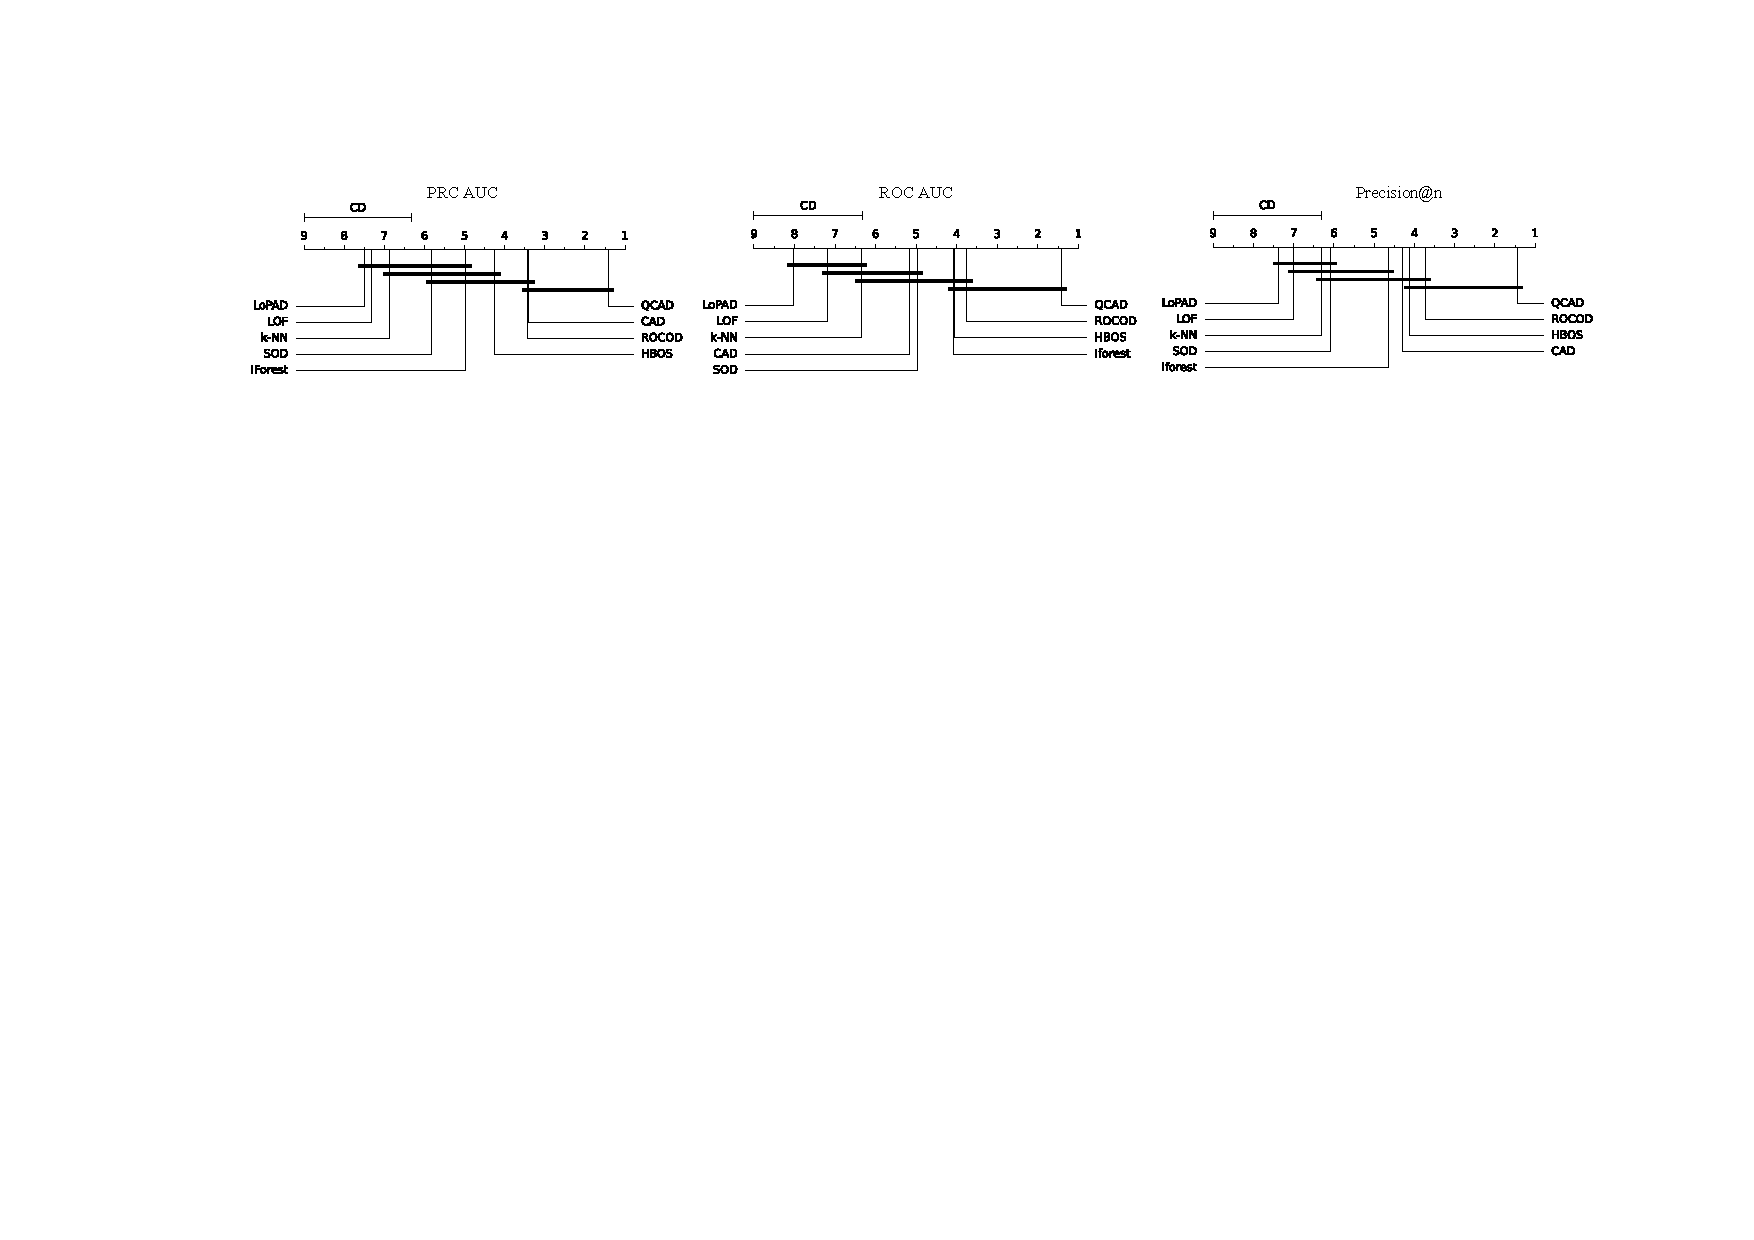
\includegraphics[width=12cm]{images/Pic_StatCom.pdf}
\caption{Biểu đồ khác biệt quan trọng thể hiện sự so sánh khác biệt thống kê giữa QCAD và các đối thủ của nó về PRC AUC, ROC AUC và Precision@n. Để đạt được điều này, chúng tôi sử dụng các bài kiểm tra Friedman \citep{friedman1937use}, sau đó là phân tích hậu kỳ Nemenyi \citep{nemenyi1963distribution} với mức ý nghĩa $0.05$. Thử nghiệm Nemenyi hậu kiểm cho thấy không có sự khác biệt đáng kể trong QCAD, CAD và ROCOD về mặt AUC của PRC; không có sự khác biệt đáng kể trong QCAD, ROCOD, HBOS và IForest về ROC AUC; không có sự khác biệt đáng kể nào trong QCAD, ROCOD, HBOS và CAD về Precision@n. Tuy nhiên, người ta có thể thấy rằng QCAD luôn vượt trội so với các đối thủ của nó ở ba chỉ số.
}\label{fig:StatCom}
\end{figure}We also observe that QCAD performs well on datasets with varying sample size, dimensionality, and rate of injected anomalies. Specifically, QCAD achieved a high ROC AUC ($\ge 0.85$) on all datasets. Giá trị này tốt hơn nhiều so với các giá trị ROC AUC gần với $0.50$ mà ROCOD, CAD, HBOS và IForest thu được trên một số tập dữ liệu, ngụ ý rằng chúng chỉ là phỏng đoán ngẫu nhiên. In addition, QCAD attained high PRC AUC ($\ge 0.8$) and Precision@n values ($\ge 0.7$) on most datasets. The lowest PRC AUC and Precision@n value are is 0.46 and 0.49, respectively, both obtained on the Toxicity dataset. Các lý do có thể dẫn đến hiệu suất vừa phải của QCAD trên Airfoil, BodyFat, Power plant và Toxicity là: mối quan hệ phụ thuộc giữa các đặc trưng hành vi và các đặc điểm ngữ cảnh không chặt chẽ hoặc mối quan hệ phụ thuộc quá phức tạp để Rừng hồi quy phân vị có thể nắm bắt được. Tuy nhiên, ROCOD, COD, HBOS và IForest nhận được các giá trị AUC PRC nhỏ hơn các giá trị 0.70 và Precision@n nhỏ hơn 0.60 trên hầu hết các tập dữ liệu. Moreover, HBOS and IForest sometimes attain PRC AUC and Precision@n lower than 0.10, which is extremely poor. Điều này ngụ ý rằng các phương pháp phát hiện sự bất thường truyền thống không phù hợp để xác định sự bất thường theo ngữ cảnh vì chúng xử lý tất cả các đặc điểm như nhau. Hơn nữa, hiệu suất tương đối kém của ROCOD và CAD---so với phương pháp của chúng tôi---cho thấy tầm quan trọng của việc lập mô hình nhiều thuộc tính của phân bố có điều kiện hơn là chỉ giá trị trung bình.

\subsection{Phân tích thời gian chạy} \label{subsec:runtime}
\begin{figure}[!htbp]
\centering
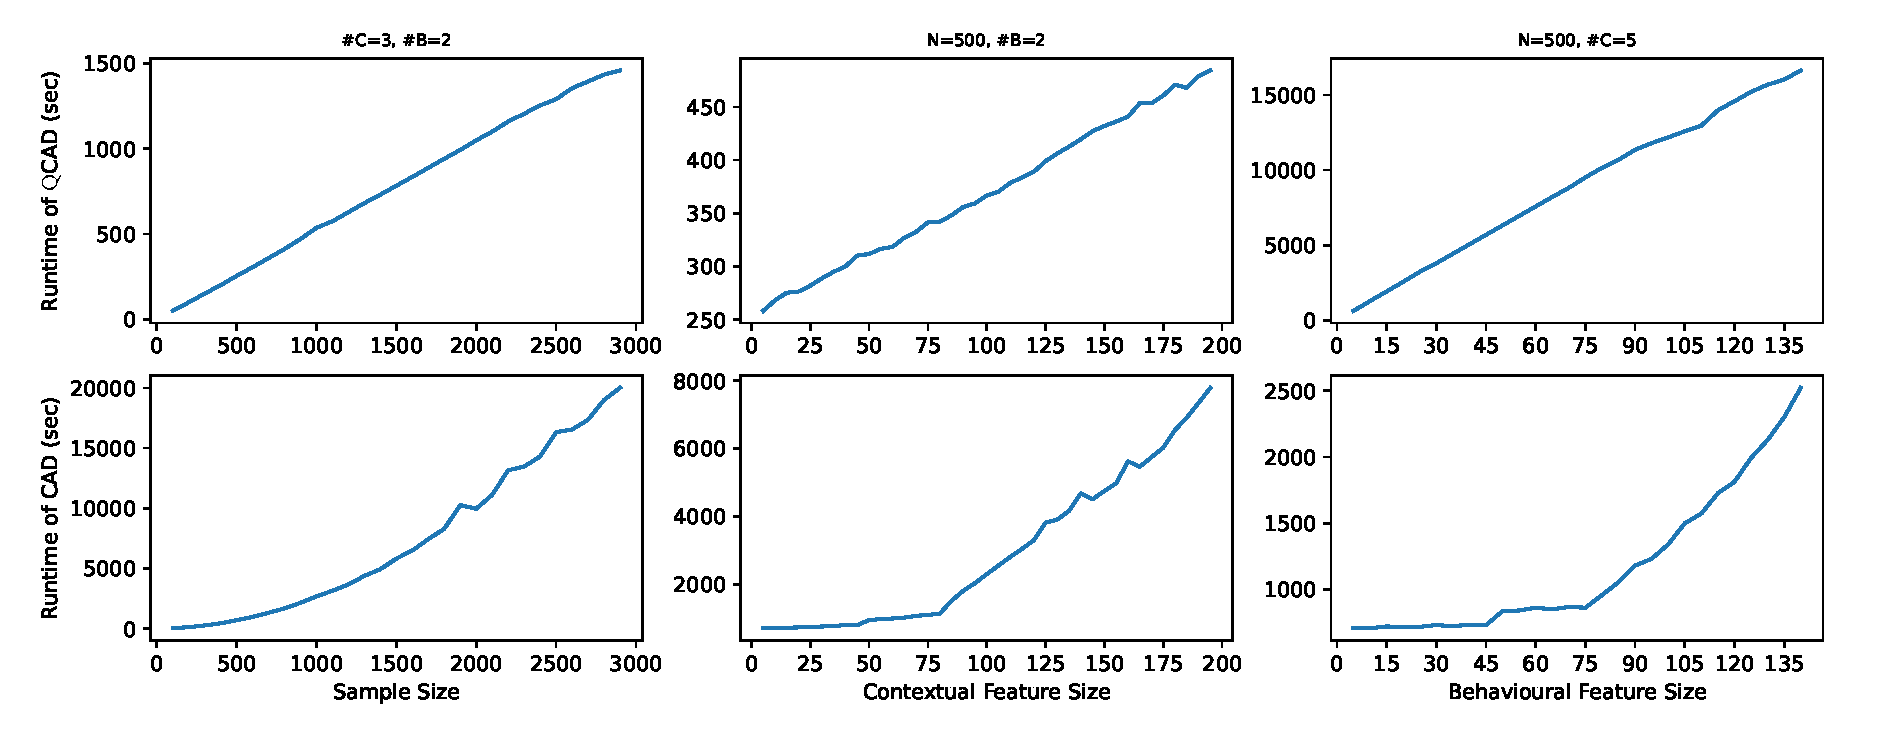
\includegraphics[width=12cm]{images/Pic_runtime.pdf}
\caption{Phân tích thời gian chạy bằng cách thay đổi kích thước mẫu, số lượng đặc trưng ngữ cảnh ($\#\textbf{C}$) và số lượng đặc trưng hành vi ($\#\textbf{B}$). Kết quả thu được từ các thử nghiệm độc lập 5. Dữ liệu được tổng hợp bằng sơ đồ S1. Lưu ý các tỷ lệ trục y khác nhau.}\label{fig:runtime}
\end{figure}

Để điều tra khả năng mở rộng và hiệu quả của QCAD, chúng tôi thực hiện phân tích thời gian chạy bằng cách thay đổi kích thước mẫu, số lượng đặc trưng ngữ cảnh và số lượng đặc trưng hành vi. Như được hiển thị trong Hình ~ \ref{fig:runtime}, chúng ta có thể quan sát bằng thực nghiệm rằng thời gian chạy của QCAD tỷ lệ tuyến tính đối với kích thước mẫu, số lượng đặc trưng ngữ cảnh và số lượng đặc trưng hành vi trên các tập dữ liệu vừa và nhỏ. In contrast, CAD is computationally prohibitively expensive even on small datasets. To further understand the complexity of QCAD, we perform a time complexity analysis in Appendix~\ref{Appendix:Complexity}. The theoretical analysis is in line with our empirical results and analysis.

\subsection{Using QCAD to Find Promising Football Players}
\label{subsec:application}

Trong phần này, chúng tôi minh họa khả năng của QCAD trong việc xác định các bất thường theo ngữ cảnh có ý nghĩa tiềm ẩn và đưa ra các giải thích trực quan và dễ hiểu cho các bất thường được báo cáo khi áp dụng cho một vấn đề trong thế giới thực.\begin{figure}[!htbp]
\centering
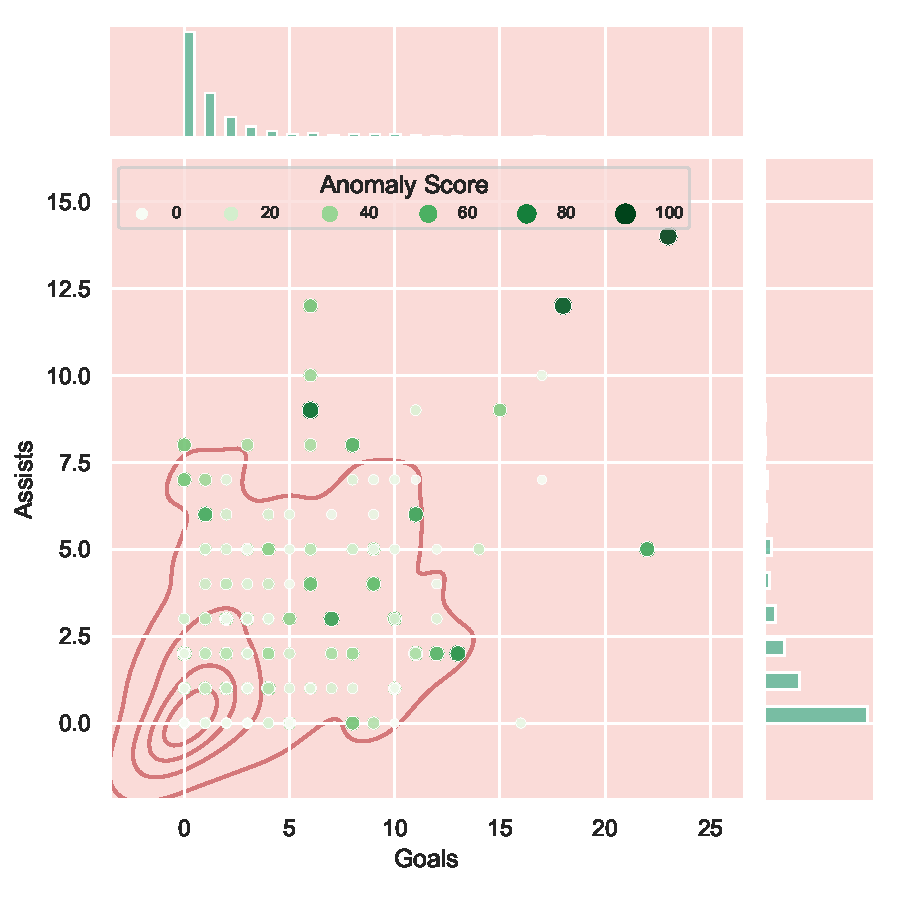
\includegraphics[width=8cm]{images/Pic_football1.pdf}
\caption{Sự phân bố của tất cả người chơi trong không gian hành vi $Assists \times Goals$ và điểm bất thường tương ứng của họ do QCAD đưa ra. Các đường cong màu đỏ biểu thị mật độ ước tính của phân bố chung ở các cấp độ khác nhau, biểu đồ biểu thị phân bố cận biên. Dấu chấm màu xanh lục lớn hơn và đậm hơn biểu thị điểm bất thường lớn hơn do QCAD đưa ra. }\label{fig:football1}
\end{figure}

Trong trường hợp sử dụng, chúng tôi xem xét vấn đề tìm kiếm những cầu thủ xuất sắc ở Giải Ngoại hạng Anh. Tập dữ liệu\footnote{https://www.kaggle.com/rajatrc1705/english-premier-league202021} mô tả thông tin cơ bản và thống kê hiệu suất của các cầu thủ bóng đá 532 từ 2020 đến 2021. Chúng tôi sử dụng các biến \textit{Position1,Position2} (vị trí mà người chơi chơi), \textit{Age} (tuổi của người chơi), \textit{Matches} (số trận đấu đã chơi), \textit{Starts} (số trận đấu mà người chơi có trong đội hình xuất phát) và \textit{Mins} (tổng số phút người chơi đã chơi) dưới dạng các đặc trưng ngữ cảnh. Hai số liệu thống kê về hiệu suất, \textit{Mục tiêu} (số bàn thắng mà cầu thủ ghi được) và \textit{Hỗ trợ} (số đường kiến ​​tạo do cầu thủ thực hiện), được coi là các đặc trưng hành vi.

Hình \ref{fig:football1} mô tả sự phân bố của tất cả các đối tượng dữ liệu trong không gian hành vi $Goals\times Assists$. Không xem xét thông tin theo ngữ cảnh, các máy phát hiện bất thường truyền thống như HBOS, LOF, IForest sẽ coi các vật thể trong khu vực dày đặc (tức là các vật thể nằm bên trong các đường cong màu đỏ) như các vật thể bình thường. Ngược lại, bộ phát hiện bất thường theo ngữ cảnh QCAD của chúng tôi có thể phát hiện các điểm bất thường ở các khu vực dày đặc bằng cách xem xét thông tin theo ngữ cảnh (tức là các vật thể màu xanh lá cây nằm bên trong các đường cong màu đỏ). Cụ thể, Hình~\ref{fig:football1} cũng trình bày điểm bất thường do QCAD đưa ra (với cài đặt mặc định). Ví dụ: người chơi Matheus Pereira---người đã đạt được các mục tiêu 11 và hỗ trợ 6---được QCAD báo cáo là 'bất thường' (tức là có điểm bất thường tương đối cao) nhưng lại là 'bình thường' bởi các máy phát hiện bất thường truyền thống. Ngược lại, QCAD coi Patrick Bamford, một cầu thủ có các bàn thắng 17 và kiến ​​tạo 7 (trong một khu vực thưa thớt), là bình thường, trong khi các máy phát hiện bất thường truyền thống coi anh ta là một kẻ dị thường.


\begin{figure}[!htbp]
\centering
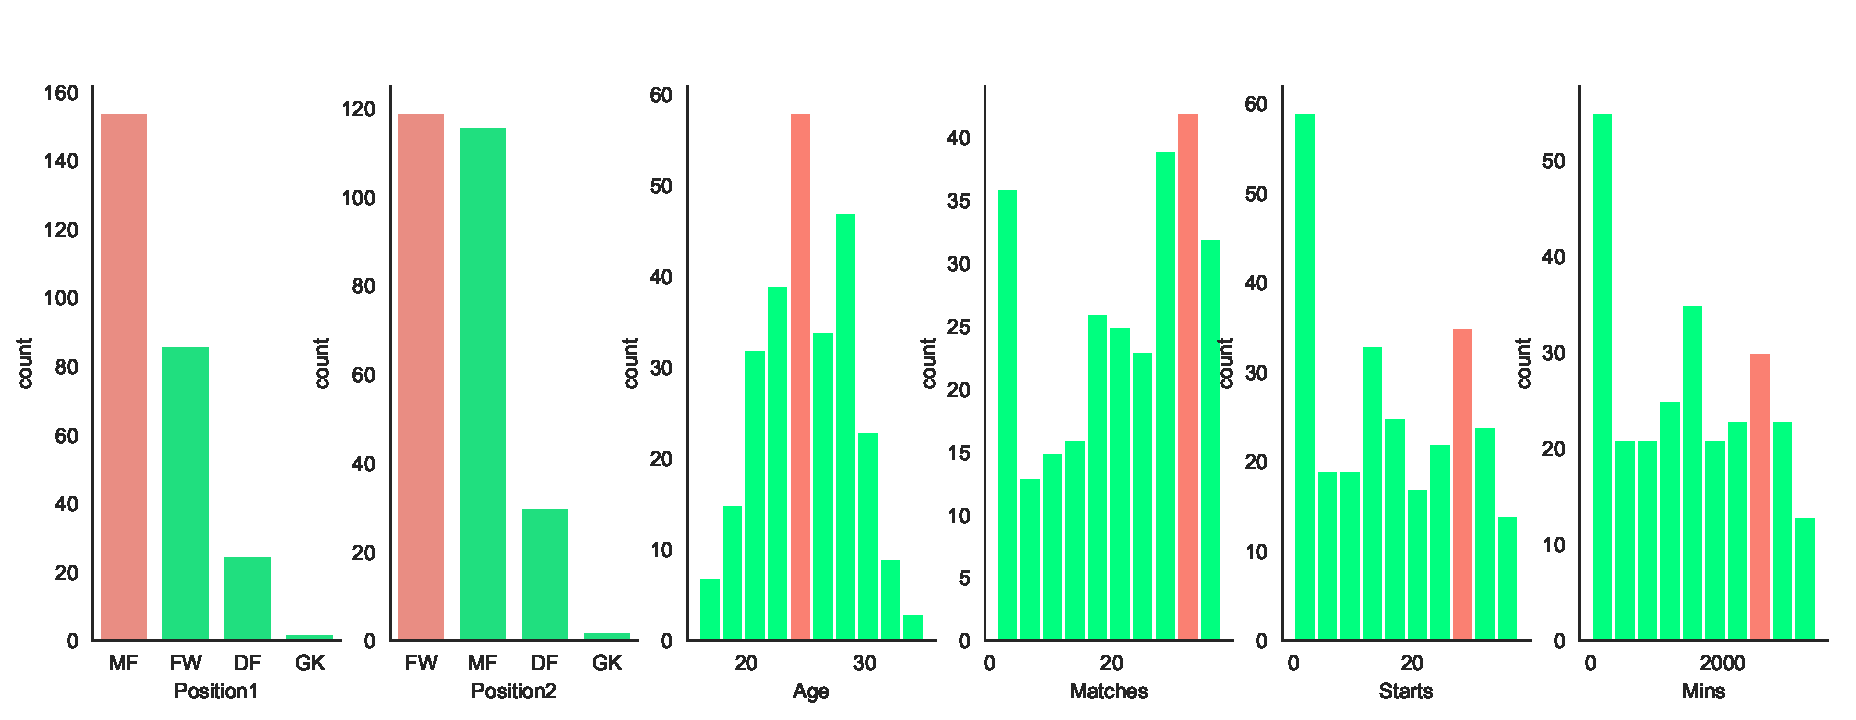
\includegraphics[width=12cm]{images/Pic_football2.pdf}
\caption{Giải thích cho người chơi dị thường được xác định là Matheus Pereira dựa trên nhóm tham chiếu của anh ta. Hiển thị là các giá trị của Matheus Pereira (thùng màu đỏ) liên quan đến việc phân bổ các lân cận theo ngữ cảnh của anh ấy cho từng đặc trưng ngữ cảnh.}\label{fig:football2}
\end{figure}


\begin{figure}[!htbp]
\centering
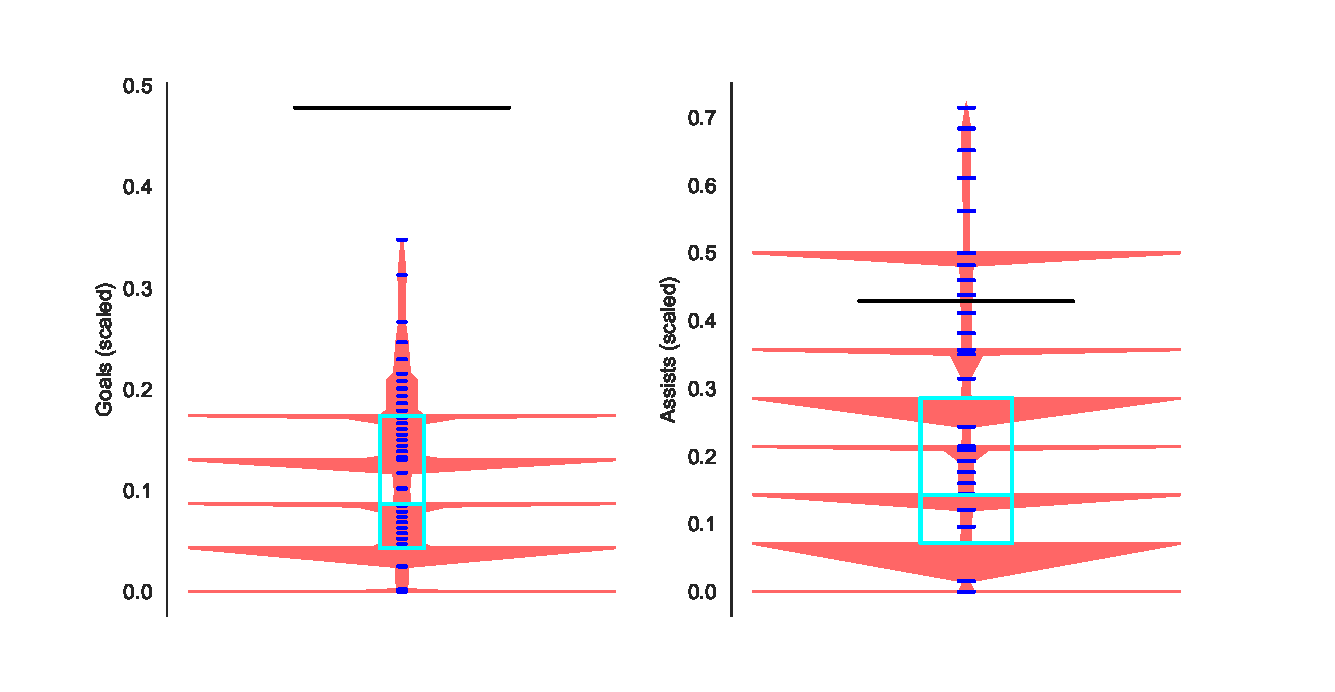
\includegraphics[width=12cm]{images/Pic_football3.pdf}
\caption{Giải thích lý do tại sao Matheus Pereira được coi là một điều bất thường: đặc biệt có nhiều bàn thắng so với những cầu thủ có bối cảnh tương tự và tương đối nhiều đường kiến tạo. Beanplot hiển thị mức phân bổ có điều kiện ước tính của từng đặc trưng hành vi, với vùng màu đỏ rộng hơn biểu thị xác suất xảy ra cao hơn. Các đường ngang màu đen biểu thị các giá trị được báo cáo cho người chơi đang được điều tra.}\label{fig:football3}
\end{figure}Ngoài việc đưa ra điểm bất thường cho từng đối tượng dữ liệu, QCAD cũng có thể đưa ra lời giải thích. Ví dụ: đối với Matheus Pereira ($Position1$ = "MF", $Position2$ = "FW", $Age$=24, $Matches$=33, $Starts$=30, $Mins$=2577), Hình~\ref{fig:football2} hiển thị sự phân bổ giá trị của từng đặc điểm ngữ cảnh cho tất cả người chơi trong vùng lân cận theo ngữ cảnh của anh ta (tức là những người chơi tương tự). Có thể thấy, hầu hết những cầu thủ này đều là Tiền vệ (MF) và/hoặc Tiền đạo (FW), có độ tuổi từ 22 đến 28, thi đấu nhiều trận hơn 25 lần, v.v. Điểm dị thường là 65.8, đưa cầu thủ này vào top-$10$ của hầu hết các cầu thủ dị thường. Điểm này có thể được phân tách theo các đặc trưng hành vi để đưa ra (các) đặc trưng hành vi đóng góp nhiều nhất vào điểm bất thường thu được; \emph{Mục tiêu}, trong trường hợp này. Hơn nữa, Hình~\ref{fig:football3} cho thấy cách trực quan hóa giống như Beanplot có thể giúp cung cấp cái nhìn sâu sắc về cách các giá trị đặc trưng hành vi khác với các giá trị trong vùng lân cận theo ngữ cảnh của người chơi. Từ những biểu đồ này, chúng ta có thể thấy rằng Matheus Pereira đặc biệt giỏi trong việc ghi bàn và tốt hơn một chút so với mong đợi về khả năng kiến ​​tạo.

Những kết quả này có thể được hiểu là: Matheus Pereira thể hiện tốt một cách đáng ngạc nhiên về số bàn thắng và tốt hơn một chút so với mong đợi về số lần kiến ​​tạo khi so sánh với các tiền vệ và/hoặc tiền đạo khác ở độ tuổi 22-28, người đã chơi nhiều hơn 25 số phút và chơi nhiều hơn 2000 số phút. Mặc dù chúng tôi không phải là chuyên gia bóng đá, nhưng chúng tôi hy vọng tính năng phát hiện tự động và giải thích tỷ số có thể hiểu được về những 'bất thường' như vậy sẽ có ý nghĩa và có thể hữu ích cho các huấn luyện viên và tuyển trạch viên bóng đá.

\section{Kết luận}
\label{sec:conclusion}

Trong bài viết này, lần đầu tiên chúng tôi thiết lập rõ ràng mối liên hệ giữa các phương pháp phát hiện bất thường truyền thống dựa trên sự phụ thuộc và các phương pháp phát hiện bất thường theo ngữ cảnh. Trên cơ sở này, chúng tôi đề xuất một cách tiếp cận mới để phát hiện và giải thích sự bất thường theo ngữ cảnh. Cụ thể, chúng tôi sử dụng Rừng hồi quy phân vị để phát triển phương pháp phát hiện bất thường chính xác và dễ hiểu, QCAD, nhằm khám phá sự phụ thuộc giữa các tính năng. QCAD có thể xử lý các tập dữ liệu dạng bảng với các đặc điểm ngữ cảnh hỗn hợp và các đặc trưng hành vi số. Kết quả thử nghiệm mở rộng trên nhiều bộ dữ liệu tổng hợp và thực tế khác nhau chứng minh rằng QCAD vượt trội hơn các phương pháp phát hiện bất thường tiên tiến nhất trong việc xác định các bất thường theo ngữ cảnh về độ chính xác và khả năng giải thích.

Từ nghiên cứu điển hình về dữ liệu cầu thủ bóng đá, chúng tôi kết luận rằng QCAD có thể phát hiện những bất thường theo ngữ cảnh có ý nghĩa và hữu ích mà chuyên gia miền có thể giải thích trực tiếp. Các hình ảnh trực quan hóa dựa trên Beanplot giúp giải thích lý do tại sao một đối tượng nhất định (không) được coi là bất thường trong bối cảnh của nó. Điều này rất quan trọng vì việc phát hiện sự bất thường là một vấn đề không được giám sát và những lời giải thích có thể giúp các nhà phân tích và chuyên gia miền xác minh kết quả. Nó cũng mở ra cơ hội phát hiện sự bất thường do con người hướng dẫn, trong đó phản hồi từ nhà phân tích có thể được sử dụng để hướng dẫn phân tích.

Trong tương lai, do QCAD chỉ có thể xử lý các tính năng tĩnh nên chúng tôi dự định mở rộng QCAD sang cài đặt phát trực tuyến.

\section*{Tuyên bố và Tuyên bố}



\bmhead{Phê duyệt đạo đức}Dữ liệu về con người và động vật liên quan đến nghiên cứu này được cung cấp công khai và do đó không cần phải phê duyệt.

\bmhead{Tài trợ}
Công việc này được hỗ trợ bởi Dự án 4 của chương trình nghiên cứu Digital Twin, một chương trình Phối cảnh TTW với số dự án P18-03 được tài trợ chủ yếu bởi Hội đồng Nghiên cứu Hà Lan (NWO). Tất cả các ý kiến, phát hiện, kết luận và khuyến nghị trong bài viết này là của các tác giả và không nhất thiết phản ánh quan điểm của các cơ quan tài trợ.

\bmhead{Xung đột lợi ích} (Các) tác giả tuyên bố không có xung đột lợi ích tiềm ẩn với
tôn trọng việc nghiên cứu, quyền tác giả và/hoặc việc xuất bản cuốn sách này
bài viết.

\bmhead{Có sẵn dữ liệu và tài liệu}
Để có thể tái tạo, toàn bộ mã và bộ dữ liệu được cung cấp tại \url{https://github.com/ZhongLIFR/QCAD}.

\bmhead{Đóng góp về quyền tác giả}

\textit{Zhong Li}: Khái niệm hóa, Phương pháp luận, Xác nhận, Điều tra, Viết, Trực quan hóa, Quản lý Dự án. \textit{Matthijs van Leeuwen}: Phương pháp luận, Xác thực, Viết, Nhận tài trợ.

\begin{thebibliography}{66}
\providecommand{\natexlab}[1]{#1}
\providecommand{\url}[1]{{#1}}
\providecommand{\urlprefix}{URL }
\providecommand{\doi}[1]{\url{https://doi.org/#1}}
\providecommand{\eprint}[2][]{\url{#2}}
 \bibcommenthead

\bibitem[{Aggarwal and Sathe(2017)}]{aggarwal2017outlier}
Aggarwal CC, Sathe S (2017) Outlier ensembles: An introduction. Springer

\bibitem[{Ahmad et~al(2017)Ahmad, Munir, Bhatti, Aftab, and
  Raza}]{ahmad2017survival}
Ahmad T, Munir A, Bhatti SH, et~al (2017) Survival analysis of heart failure
  patients: A case study. PloS one 12(7):e0181,001

\bibitem[{Ahmed et~al(2016{\natexlab{a}})Ahmed, Mahmood, and
  Hu}]{ahmed2016survey1}
Ahmed M, Mahmood AN, Hu J (2016{\natexlab{a}}) A survey of network anomaly
  detection techniques. Journal of Network and Computer Applications 60:19--31

\bibitem[{Ahmed et~al(2016{\natexlab{b}})Ahmed, Mahmood, and
  Islam}]{ahmed2016survey2}
Ahmed M, Mahmood AN, Islam MR (2016{\natexlab{b}}) A survey of anomaly
  detection techniques in financial domain. Future Generation Computer Systems
  55:278--288

\bibitem[{Angiulli and Pizzuti(2002)}]{angiulli2002fast}
Angiulli F, Pizzuti C (2002) Fast outlier detection in high dimensional spaces.
  In: European conference on principles of data mining and knowledge discovery,
  Springer, pp 15--27

\bibitem[{Babbar and Chawla(2012)}]{babbar2012mining}
Babbar S, Chawla S (2012) Mining causal outliers using gaussian bayesian
  networks. In: 2012 IEEE 24th International Conference on Tools with
  Artificial Intelligence, IEEE, pp 97--104

\bibitem[{Breiman(2001)}]{breiman2001random}
Breiman L (2001) Random forests. Machine learning 45:5--32

\bibitem[{Breiman et~al(2017)Breiman, Friedman, Olshen, and
  Stone}]{breiman2017classification}
Breiman L, Friedman JH, Olshen RA, et~al (2017) Classification and regression
  trees. Routledge

\bibitem[{Breunig et~al(2000)Breunig, Kriegel, Ng, and Sander}]{breunig2000lof}
Breunig MM, Kriegel HP, Ng RT, et~al (2000) Lof: identifying density-based
  local outliers. In: Proceedings of the 2000 ACM SIGMOD international
  conference on Management of data, pp 93--104

\bibitem[{Buczak and Guven(2015)}]{buczak2015survey}
Buczak AL, Guven E (2015) A survey of data mining and machine learning methods
  for cyber security intrusion detection. IEEE Communications surveys \&
  tutorials 18(2):1153--1176

\bibitem[{Cabero et~al(2021)Cabero, Epifanio, Pi{\'e}rola, and
  Ballester}]{cabero2021archetype}
Cabero I, Epifanio I, Pi{\'e}rola A, et~al (2021) Archetype analysis: A new
  subspace outlier detection approach. Knowledge-Based Systems 217:106,830

\bibitem[{Cai et~al(2013)Cai, He, and Man}]{cai2013spatial}
Cai Q, He H, Man H (2013) Spatial outlier detection based on iterative
  self-organizing learning model. Neurocomputing 117:161--172

\bibitem[{Calikus et~al(2021)Calikus, Nowaczyk, Bouguelia, and
  Dikmen}]{calikus2021wisdom}
Calikus E, Nowaczyk S, Bouguelia MR, et~al (2021) Wisdom of the contexts:
  Active ensemble learning for contextual anomaly detection. arXiv preprint
  arXiv:210111560

\bibitem[{Campos et~al(2016)Campos, Zimek, Sander, Campello, Micenkov{\'a},
  Schubert, Assent, and Houle}]{campos2016evaluation}
Campos GO, Zimek A, Sander J, et~al (2016) On the evaluation of unsupervised
  outlier detection: measures, datasets, and an empirical study. Data mining
  and knowledge discovery 30(4):891--927

\bibitem[{Chandola et~al(2009)Chandola, Banerjee, and
  Kumar}]{chandola2009anomaly}
Chandola V, Banerjee A, Kumar V (2009) Anomaly detection: A survey. ACM
  computing surveys (CSUR) 41(3):1--58

\bibitem[{F{\"a}rber et~al(2010)F{\"a}rber, G{\"u}nnemann, Kriegel, Kr{\"o}ger,
  M{\"u}ller, Schubert, Seidl, and Zimek}]{farber2010using}
F{\"a}rber I, G{\"u}nnemann S, Kriegel HP, et~al (2010) On using class-labels
  in evaluation of clusterings. In: MultiClust: 1st international workshop on
  discovering, summarizing and using multiple clusterings held in conjunction
  with KDD, p~1

\bibitem[{Fokkema et~al(2022)Fokkema, de~Heide, and van
  Erven}]{fokkema2022attribution}
Fokkema H, de~Heide R, van Erven T (2022) Attribution-based explanations that
  provide recourse cannot be robust. arXiv preprint arXiv:220515834

\bibitem[{Friedman(1937)}]{friedman1937use}
Friedman M (1937) The use of ranks to avoid the assumption of normality
  implicit in the analysis of variance. Journal of the american statistical
  association 32(200):675--701

\bibitem[{Goldstein and Dengel(2012)}]{goldstein2012histogram}
Goldstein M, Dengel A (2012) Histogram-based outlier score (hbos): A fast
  unsupervised anomaly detection algorithm. KI-2012: Poster and Demo Track pp
  59--63

\bibitem[{Gower(1971)}]{gower1971general}
Gower JC (1971) A general coefficient of similarity and some of its properties.
  Biometrics pp 857--871

\bibitem[{Harrison~Jr and Rubinfeld(1978)}]{harrison1978hedonic}
Harrison~Jr D, Rubinfeld DL (1978) Hedonic housing prices and the demand for
  clean air. Journal of environmental economics and management 5(1):81--102

\bibitem[{Hawkins(1980)}]{hawkins1980identification}
Hawkins DM (1980) Identification of outliers, vol~11. Springer

\bibitem[{Hayes and Capretz(2014)}]{hayes2014contextual}
Hayes MA, Capretz MA (2014) Contextual anomaly detection in big sensor data.
  In: 2014 IEEE International Congress on Big Data, IEEE, pp 64--71

\bibitem[{Hong and Hauskrecht(2015)}]{hong2015multivariate}
Hong C, Hauskrecht M (2015) Multivariate conditional anomaly detection and its
  clinical application. In: Proceedings of the AAAI Conference on Artificial
  Intelligence

\bibitem[{Huang et~al(2003)Huang, Fan, Lee, and Yu}]{huang2003cross}
Huang Ya, Fan W, Lee W, et~al (2003) Cross-feature analysis for detecting
  ad-hoc routing anomalies. In: 23rd International Conference on Distributed
  Computing Systems, 2003. Proceedings., IEEE, pp 478--487

\bibitem[{Hwang et~al(2009)Hwang, Kim, Kim, and Seah}]{hwang2009survey}
Hwang I, Kim S, Kim Y, et~al (2009) A survey of fault detection, isolation, and
  reconfiguration methods. IEEE transactions on control systems technology
  18(3):636--653

\bibitem[{Kampstra(2008)}]{kampstra2008beanplot}
Kampstra P (2008) Beanplot: A boxplot alternative for visual comparison of
  distributions. Journal of statistical software 28(1):1--9

\bibitem[{Kandanaarachchi et~al(2020)Kandanaarachchi, Mu{\~n}oz, Hyndman, and
  Smith-Miles}]{kandanaarachchi2020normalization}
Kandanaarachchi S, Mu{\~n}oz MA, Hyndman RJ, et~al (2020) On normalization and
  algorithm selection for unsupervised outlier detection. Data Mining and
  Knowledge Discovery 34(2):309--354

\bibitem[{Koenker and Hallock(2001)}]{koenker2001quantile}
Koenker R, Hallock KF (2001) Quantile regression. Journal of economic
  perspectives 15(4):143--156

\bibitem[{Kriegel et~al(2009)Kriegel, Kr{\"o}ger, Schubert, and
  Zimek}]{kriegel2009outlier}
Kriegel HP, Kr{\"o}ger P, Schubert E, et~al (2009) Outlier detection in
  axis-parallel subspaces of high dimensional data. In: Pacific-asia conference
  on knowledge discovery and data mining, Springer, pp 831--838

\bibitem[{Kriegel et~al(2012)Kriegel, Kr{\"o}ger, Schubert, and
  Zimek}]{kriegel2012outlier}
Kriegel HP, Kr{\"o}ger P, Schubert E, et~al (2012) Outlier detection in
  arbitrarily oriented subspaces. In: 2012 IEEE 12th international conference
  on data mining, IEEE, pp 379--388

\bibitem[{Kuo et~al(2018)Kuo, Li, and Kifer}]{kuo2018detecting}
Kuo YH, Li Z, Kifer D (2018) Detecting outliers in data with correlated
  measures. In: Proceedings of the 27th ACM International Conference on
  Information and Knowledge Management, pp 287--296

\bibitem[{Lei et~al(2018)Lei, G’Sell, Rinaldo, Tibshirani, and
  Wasserman}]{lei2018distribution}
Lei J, G’Sell M, Rinaldo A, et~al (2018) Distribution-free predictive
  inference for regression. Journal of the American Statistical Association
  113(523):1094--1111

\bibitem[{Li et~al(2022)Li, Zhu, and van Leeuwen}]{li2022survey}
Li Z, Zhu Y, van Leeuwen M (2022) A survey on explainable anomaly detection.
  arXiv preprint arXiv:221006959

\bibitem[{Liang and Parthasarathy(2016)}]{liang2016robust}
Liang J, Parthasarathy S (2016) Robust contextual outlier detection: Where
  context meets sparsity. In: Proceedings of the 25th ACM International on
  Conference on Information and Knowledge Management, pp 2167--2172

\bibitem[{Liu et~al(2008)Liu, Ting, and Zhou}]{liu2008isolation}
Liu FT, Ting KM, Zhou ZH (2008) Isolation forest. In: 2008 eighth ieee
  international conference on data mining, IEEE, pp 413--422

\bibitem[{Liu et~al(2018)Liu, Shin, and Hu}]{liu2018contextual}
Liu N, Shin D, Hu X (2018) Contextual outlier interpretation. In: Proceedings
  of the 27th International Joint Conference on Artificial Intelligence, pp
  2461--2467

\bibitem[{Lu et~al(2020{\natexlab{a}})Lu, Liu, Li, Le, and
  Liu}]{lu2020dependency}
Lu S, Liu L, Li J, et~al (2020{\natexlab{a}}) Dependency-based anomaly
  detection: Framework, methods and benchmark. arXiv preprint arXiv:201106716

\bibitem[{Lu et~al(2020{\natexlab{b}})Lu, Liu, Li, Le, and Liu}]{lu2020lopad}
Lu S, Liu L, Li J, et~al (2020{\natexlab{b}}) Lopad: A local prediction
  approach to anomaly detection. Advances in Knowledge Discovery and Data
  Mining 12085:660

\bibitem[{Lundberg and Lee(2017)}]{lundberg2017unified}
Lundberg SM, Lee SI (2017) A unified approach to interpreting model
  predictions. Advances in neural information processing systems 30

\bibitem[{Meghanath et~al(2018)Meghanath, Pai, and
  Akoglu}]{meghanath2018conout}
Meghanath M, Pai D, Akoglu L (2018) Conout: Con textual outlier detection with
  multiple contexts: Application to ad fraud. In: Joint European Conference on
  Machine Learning and Knowledge Discovery in Databases, Springer, pp 139--156

\bibitem[{Meinshausen(2006)}]{meinshausen2006quantile}
Meinshausen N (2006) Quantile regression forests. Journal of Machine Learning
  Research 7(6):983--999

\bibitem[{Micenkov{\'a} et~al(2014)Micenkov{\'a}, McWilliams, and
  Assent}]{micenkova2014learning}
Micenkov{\'a} B, McWilliams B, Assent I (2014) Learning outlier ensembles: The
  best of both worlds--supervised and unsupervised. In: Proceedings of the ACM
  SIGKDD 2014 Workshop on Outlier Detection and Description under Data
  Diversity (ODD2). New York, NY, USA, Citeseer, pp 51--54

\bibitem[{Micenkov{\'a} et~al(2015)Micenkov{\'a}, McWilliams, and
  Assent}]{micenkova2015learning}
Micenkov{\'a} B, McWilliams B, Assent I (2015) Learning representations for
  outlier detection on a budget. arXiv preprint arXiv:150708104

\bibitem[{Nemenyi(1963)}]{nemenyi1963distribution}
Nemenyi PB (1963) Distribution-free multiple comparisons. Princeton University

\bibitem[{Nguyen et~al(2013)Nguyen, M{\"u}ller, Vreeken, Keller, and
  B{\"o}hm}]{nguyen2013cmi}
Nguyen HV, M{\"u}ller E, Vreeken J, et~al (2013) Cmi: An information-theoretic
  contrast measure for enhancing subspace cluster and outlier detection. In:
  Proceedings of the 2013 SIAM International Conference on Data Mining, SIAM,
  pp 198--206

\bibitem[{Noto et~al(2010)Noto, Brodley, and Slonim}]{noto2010anomaly}
Noto K, Brodley C, Slonim D (2010) Anomaly detection using an ensemble of
  feature models. In: 2010 ieee international conference on data mining, IEEE,
  pp 953--958

\bibitem[{Pang et~al(2021)Pang, Shen, Cao, and Hengel}]{pang2021deep}
Pang G, Shen C, Cao L, et~al (2021) Deep learning for anomaly detection: A
  review. ACM Computing Surveys (CSUR) 54(2):1--38

\bibitem[{Panjei et~al(2022)Panjei, Gruenwald, Leal, Nguyen, and
  Silvia}]{panjei2022survey}
Panjei E, Gruenwald L, Leal E, et~al (2022) A survey on outlier explanations.
  The VLDB Journal 31(5):977--1008

\bibitem[{Pasillas-D{\'\i}az and Ratt{\'e}(2016)}]{pasillas2016unsupervised}
Pasillas-D{\'\i}az JR, Ratt{\'e} S (2016) An unsupervised approach for
  combining scores of outlier detection techniques, based on similarity
  measures. Electronic notes in theoretical computer science 329:61--77

\bibitem[{Salvador et~al(2004)Salvador, Chan, and
  Brodie}]{salvador2004learning}
Salvador S, Chan P, Brodie J (2004) Learning states and rules for time series
  anomaly detection. In: FLAIRS conference, pp 306--311

\bibitem[{Scutari et~al(2019)Scutari, Scutari, and MMPC}]{scutari2019package}
Scutari M, Scutari MM, MMPC HP (2019) Package ‘bnlearn’. Bayesian network
  structure learning, parameter learning and inference, R package version 4(1)

\bibitem[{Segal and Xiao(2011)}]{segal2011multivariate}
Segal M, Xiao Y (2011) Multivariate random forests. Wiley interdisciplinary
  reviews: Data mining and knowledge discovery 1(1):80--87

\bibitem[{Seger(2018)}]{seger2018investigation}
Seger C (2018) An investigation of categorical variable encoding techniques in
  machine learning: binary versus one-hot and feature hashing

\bibitem[{Smets et~al(2009)Smets, Verdonk, and Jordaan}]{smets2009discovering}
Smets K, Verdonk B, Jordaan EM (2009) Discovering novelty in spatio/temporal
  data using one-class support vector machines. In: 2009 International Joint
  Conference on Neural Networks, IEEE, pp 2956--2963

\bibitem[{Song et~al(2007)Song, Wu, Jermaine, and Ranka}]{song2007conditional}
Song X, Wu M, Jermaine C, et~al (2007) Conditional anomaly detection. IEEE
  Transactions on knowledge and Data Engineering 19(5):631--645

\bibitem[{Spinosa and Carvalho(2005)}]{spinosa2005support}
Spinosa EJ, Carvalho A (2005) Support vector machines for novel class detection
  in bioinformatics. Genet Mol Res 4(3):608--15

\bibitem[{Tang et~al(2015)Tang, Pei, Bailey, and Dong}]{tang2015mining}
Tang G, Pei J, Bailey J, et~al (2015) Mining multidimensional contextual
  outliers from categorical relational data. Intelligent Data Analysis
  19(5):1171--1192

\bibitem[{Teng(1999)}]{teng1999correcting}
Teng CM (1999) Correcting noisy data. In: ICML, Citeseer, pp 239--248

\bibitem[{Valko et~al(2011)Valko, Kveton, Valizadegan, Cooper, and
  Hauskrecht}]{valko2011conditional}
Valko M, Kveton B, Valizadegan H, et~al (2011) Conditional anomaly detection
  with soft harmonic functions. In: 2011 IEEE 11th International Conference on
  Data Mining, IEEE, pp 735--743

\bibitem[{Wang et~al(2019)Wang, Bah, and Hammad}]{wang2019progress}
Wang H, Bah MJ, Hammad M (2019) Progress in outlier detection techniques: A
  survey. Ieee Access 7:107,964--108,000

\bibitem[{Wong et~al(2003)Wong, Moore, Cooper, and Wagner}]{wong2003bayesian}
Wong WK, Moore AW, Cooper GF, et~al (2003) Bayesian network anomaly pattern
  detection for disease outbreaks. In: Proceedings of the 20th International
  Conference on Machine Learning (ICML-03), pp 808--815

\bibitem[{Xu et~al(2021)Xu, Wang, Jian, Huang, Wang, Liu, and
  Li}]{xu2021beyond}
Xu H, Wang Y, Jian S, et~al (2021) Beyond outlier detection: Outlier
  interpretation by attention-guided triplet deviation network. In: Proceedings
  of the Web Conference 2021, pp 1328--1339

\bibitem[{Yaramakala and Margaritis(2005)}]{yaramakala2005speculative}
Yaramakala S, Margaritis D (2005) Speculative markov blanket discovery for
  optimal feature selection. In: Fifth IEEE International Conference on Data
  Mining (ICDM'05), IEEE, pp 4--pp

\bibitem[{Zhao et~al(2019)Zhao, Nasrullah, and Li}]{zhao2019pyod}
Zhao Y, Nasrullah Z, Li Z (2019) Pyod: A python toolbox for scalable outlier
  detection. Journal of Machine Learning Research 20:1--7

\bibitem[{Zheng et~al(2017)Zheng, Brantley, Lauvaux, and
  Li}]{zheng2017contextual}
Zheng G, Brantley SL, Lauvaux T, et~al (2017) Contextual spatial outlier
  detection with metric learning. In: Proceedings of the 23rd ACM SIGKDD
  International Conference on Knowledge Discovery and Data Mining, pp
  2161--2170

\end{thebibliography}



\appendix

\section{Phân tích độ phức tạp}\label{Appendix:Complexity}
Chi phí tính toán của khung QCAD của chúng tôi chủ yếu đến từ hai phần: tính toán ma trận Khoảng cách của Gower bằng cách sử dụng các đặc trưng ngữ cảnh và tính toán điểm bất thường bằng cách sử dụng tất cả các tính năng dựa trên Rừng hồi quy phân vị.

Độ phức tạp về thời gian của việc tính toán ma trận Khoảng cách của Gower là $O(N^{2}D_{cnt})$, trong đó $N$ biểu thị kích thước mẫu và $D_{cnt}$ biểu thị số lượng đặc trưng ngữ cảnh. Ngoài ra, độ phức tạp về thời gian của việc xây dựng một khu rừng ngẫu nhiên là $O( n_{tree}\cdot n_{feature} \cdot k log(k))$ và sử dụng nó để dự đoán là $O( n_{tree}\cdot n_{feature})$ \citep{buczak2015survey}, trong đó $n_{tree}$ là số cây được sử dụng để tạo thành một khu rừng ngẫu nhiên, $n_{feature}$ biểu thị số thứ nguyên (tức là nhiều nhất là $D_{cnt}$) và $k$ cho biết số lượng mẫu được sử dụng để xây dựng khu rừng (tức là số lượng hàng xóm gần nhất trong trường hợp của chúng tôi). Do đó, độ phức tạp về thời gian của việc xây dựng các khu rừng hồi quy phân vị $N$ trong các đặc trưng hành vi của $D_{bhv}$ là $O( n_{tree}\cdot D_{cnt} \cdot k log(k) \cdot N \cdot D_{bhv} )$.
Hơn nữa, chúng tôi phải ước tính $100$ các lượng tử khác nhau bằng cách sử dụng từng rừng hồi quy phân vị, dẫn đến $O( (n_{tree} \cdot D_{cnt} \cdot k log(k)+ n_{tree} \cdot D_{cnt} \cdot 100) \cdot N \cdot D_{bhv} )$. Do đó, việc sử dụng cài đặt mặc định của chúng tôi sẽ dẫn đến $O( ( 100 \cdot D_{cnt} \cdot \mathrm{min}(500,\frac{N}{2})\cdot \mathrm{log}(\mathrm{min}(500,\frac{N}{2})) + 100 \cdot D_{cnt} \cdot 100) \cdot N \cdot D_{bhv})$. Trường hợp xấu nhất là $O(10^{5}N D_{cnt}D_{bhv}).$

Nhìn chung, độ phức tạp về thời gian của phương pháp của chúng tôi là $O(10^{5}N D_{cnt}D_{bhv}+N^{2}D_{cnt})$ trong trường hợp xấu nhất. Đặc biệt, độ phức tạp về thời gian trở thành $O(10^{5}N D_{cnt}D_{bhv})$ khi $N<10^{5}$ (tức là đối với các tập dữ liệu vừa và nhỏ). Ngoài ra, việc xây dựng các khu rừng hồi quy phân vị cho từng đối tượng trong từng đặc trưng hành vi có thể dễ dàng được thực hiện theo cách song song, do đó giảm độ phức tạp về thời gian xuống $O(10^{5}N D_{cnt}+N^{2}D_{cnt})$ trong trường hợp xấu nhất.

\section{Mô tả tập dữ liệu}\label{Appendix:Data}

\paragraph{Bào ngư} Tập dữ liệu chứa các bản ghi đo vật lý bào ngư 4177. Cụ thể, chúng tôi sử dụng các đặc điểm Giới tính, Chiều dài, Đường kính và Chiều cao làm đặc trưng ngữ cảnh. Theo đó, chúng tôi sử dụng các đặc điểm Trọng lượng Toàn bộ, Trọng lượng Shucked, Trọng lượng Nội tạng, Trọng lượng Vỏ và Vòng làm các đặc trưng hành vi. Tập dữ liệu này được tải xuống từ UCI, \footnote{https://archive.ics.uci.edu/ml/datasets/abalone} không chứa giá trị nào bị thiếu.


\paragraph{Độ ồn của cánh máy bay} Tập dữ liệu này chứa các bản ghi 1503 từ một loạt các thử nghiệm khí động học và âm thanh của các phần cánh cánh máy bay. Cụ thể, chúng tôi sử dụng các tính năng mô tả tần số, góc tấn công, độ dài hợp âm, vận tốc dòng tự do và độ dày dịch chuyển phía hút (ví dụ: f, alpha, c, U\_infinity và delta) làm các đặc trưng ngữ cảnh. Trong khi đó, tính năng mô tả mức áp suất âm thanh được chia tỷ lệ (ví dụ: SSPL) là đặc trưng hành vi. Tập dữ liệu này được tải xuống từ UCI, \footnote{https://archive.ics.uci.edu/ml/datasets/Airfoil+Self-Noise} không chứa giá trị nào bị thiếu.\paragraph{Bodyfat} Tập dữ liệu này chứa các ước tính về mật độ cơ thể và
tỷ lệ phần trăm mỡ cơ thể (được sử dụng làm đặc trưng hành vi), được xác định bằng nhiều phép đo chu vi cơ thể khác nhau, chẳng hạn như Tuổi, Cân nặng, Chiều cao, Chu vi cổ, Chu vi ngực, Chu vi bụng 2, Chu vi hông, Chu vi đùi, Chu vi đầu gối, Chu vi mắt cá chân, Chu vi bắp tay (mở rộng), Chu vi cẳng tay và Chu vi cổ tay (được sử dụng làm đặc trưng ngữ cảnh) cho nam giới 252. Tập dữ liệu thô không bao gồm các tính năng phân loại và các giá trị bị thiếu 0, được tải xuống từ statlib CMU. \footnote{http://lib.stat.cmu.edu/datasets/bodyfat}


\paragraph{Giá nhà ở Boston} Tập dữ liệu này chứa các bản ghi 583 về giá nhà ở Boston. Chúng tôi sử dụng các đặc điểm mô tả các thuộc tính của ngôi nhà và môi trường xung quanh nó, ví dụ: CRIM, ZN, INDUS, CHAS, NOX, RM, AGE, DIS, RAD, TAX, PTRATIO, B, LSTAT làm đặc điểm ngữ cảnh và giá trị trung bình của các ngôi nhà do chủ sở hữu sử dụng, tức là MED, làm đặc trưng hành vi. Tập dữ liệu này được phát hành bởi \cite{harrison1978hedonic} và được tải xuống từ CMU statlib \footnote{http://lib.stat.cmu.edu/datasets}. Nó vẫn giữ lại các bản ghi 506 sau khi loại bỏ các hàng chứa giá trị bị thiếu.

\paragraph{Cường độ nén bê tông } Tập dữ liệu này chứa các bản ghi 1030 về cường độ nén của bê tông. Chúng tôi sử dụng các đặc điểm mô tả độ tuổi và các thành phần khác nhau làm đặc trưng ngữ cảnh, bao gồm C1, C2, C3, C4, C5, C6, C7 và Tuổi. Ngoài ra, chúng tôi sử dụng tính năng Strength làm đặc trưng hành vi. Tập dữ liệu này được tải xuống từ UCI, \footnote{https://archive.ics.uci.edu/ml/datasets/Concrete+Compressive+Strength} không chứa giá trị bị thiếu.

\paragraph{El Nino } Tập dữ liệu này chứa các bản ghi 178080 về các chỉ số khí tượng bề mặt và hải dương học, đó là
lấy từ các phao nằm khắp vùng xích đạo Thái Bình Dương. Chúng tôi sử dụng các tính năng không gian và thời gian, ví dụ: Năm, Tháng, Ngày, Ngày, Vĩ độ, Kinh độ làm các đặc trưng ngữ cảnh và các tính năng khác, ví dụ: Zonal\_Winds, Meridional\_Winds, Độ ẩm, Air\_Temp, Sea\_Surface\_Temp là các đặc trưng hành vi. Tập dữ liệu này được tải xuống từ kho lưu trữ máy học UCI.\footnote{archive.ics.uci.edu/ml/datasets/El+Nino}. Tập dữ liệu này vẫn giữ lại các bản ghi 93935 sau khi loại bỏ các hàng chứa các giá trị bị thiếu. Tuy nhiên, để tất cả các thuật toán hoàn thành thử nghiệm trên tập dữ liệu này trong vòng vài giờ 12, chúng tôi lấy mẫu ngẫu nhiên tập dữ liệu gốc xuống bản ghi 20,000.

\paragraph{Energy Efficiency} Tập dữ liệu này chứa các bản ghi 768 về một nghiên cứu đánh giá hiệu quả năng lượng như một hàm của các thông số tòa nhà. Theo đó, các tham số của tòa nhà như X1, X2, X3, X4, X5, X6, X7 và X8 được coi là các đặc trưng ngữ cảnh, còn tải sưởi ấm và tải làm mát (cụ thể là Y1 và Y2) được coi là các đặc trưng hành vi. Tập dữ liệu này được tải xuống từ UCI, \footnote{https://archive.ics.uci.edu/ml/datasets/Energy+efficiency} không chứa giá trị nào bị thiếu.\paragraph{Trọng lượng cá } Tập dữ liệu này chứa các bản ghi 157 về đặc điểm của các loài cá phổ biến trên thị trường. Theo đó, chúng tôi sử dụng các đặc điểm bao gồm Loài, Chiều dài1, Chiều dài2, Chiều dài3, Chiều cao, Chiều rộng làm đặc trưng ngữ cảnh và Trọng lượng làm đặc trưng hành vi. Tập dữ liệu này được tải xuống từ Kaggle, \footnote{https://www.kaggle.com/aungpyaeap/fish-market} không chứa giá trị nào bị thiếu.

\paragraph{Cháy rừng} Tập dữ liệu này chứa các bản ghi 517 liên quan đến thông tin khí tượng và không gian thời gian về cháy rừng ở khu vực đông bắc Bồ Đào Nha. Chúng tôi sử dụng các đặc điểm không gian theo thời gian như X, Y, tháng, ngày làm các đặc trưng ngữ cảnh và các đặc điểm còn lại, tức là FFMC, DMC, DC, ISI, nhiệt độ, RH, gió, mưa, khu vực làm các đặc trưng hành vi. Nó được tải xuống từ kho lưu trữ máy học UCI,\footnote{https://archive.ics.uci.edu/ml/datasets/forest+fires} không chứa giá trị nào bị thiếu.

\paragraph{Phát thải CO và NOx của tuabin khí } Tập dữ liệu ban đầu bao gồm các bản ghi 36733 về dữ liệu đo cảm biến, được thu thập từ một tuabin khí ở Thổ Nhĩ Kỳ từ 2011 đến 2015. Bộ dữ liệu được thu thập từ cùng một nhà máy điện để nghiên cứu lượng khí thải và dự đoán sản lượng năng lượng ròng hàng giờ. Do đó, chúng tôi sử dụng các tính năng mô tả các tham số tuabin (ví dụ: AT, AP, AH, AFDP, GTEP, TIT, TAT và CDP) làm các đặc trưng ngữ cảnh.
Các biến đặc trưng cho hiệu suất năng lượng của tuabin và lượng phát thải khí (ví dụ: TEY, CO và NOX) được sử dụng làm đặc trưng hành vi. Tuy nhiên, để tất cả các thuật toán hoàn thành thử nghiệm trong vòng 12 giờ, chúng tôi chỉ sử dụng các bản ghi 7383 trong 2015. Tập dữ liệu này được tải xuống từ UCI, \footnote{https://archive.ics.uci.edu/ml/datasets/Gas+Turbine+CO+and+NOx+Emission+Data+Set} không chứa giá trị bị thiếu.


\paragraph{Suy tim}
Tập dữ liệu này chứa hồ sơ lâm sàng về bệnh suy tim của bệnh nhân 299 bị suy tim. Nó chứa các đặc điểm lâm sàng 13, trong đó chúng tôi sử dụng tuổi tác, giới tính, hút thuốc, bệnh tiểu đường, \_blood\_áp lực và thiếu máu làm đặc trưng ngữ cảnh và creatinine\_phosphokinase, ejection\_phân đoạn, tiểu cầu, huyết thanh\_creatinine, huyết thanh\_sodium, thời gian là đặc trưng hành vi. Ngoài ra, tính năng death\_event đã bị xóa và không có giá trị nào bị thiếu trong tập dữ liệu này. Tập dữ liệu gốc được phát hành bởi \cite{ahmad2017survival} và chúng tôi tải xuống từ kho lưu trữ máy học UCI. \footnote{archive.ics.uci.edu/ml/datasets/Heart+failure+clinical+records}

\paragraph{Viêm gan}
Tập dữ liệu này chứa các bản ghi 615 liên quan đến giá trị xét nghiệm của người hiến máu và bệnh nhân Viêm gan C. Chúng tôi sử dụng các đặc điểm nhân khẩu học như giới tính và độ tuổi cũng như Danh mục nhà tài trợ làm đặc điểm ngữ cảnh và các đặc điểm còn lại, tức là ALB, ALP, ALT, AST, BIL, CHE, CHOL, CREA, GGT và PROT làm đặc trưng hành vi. Tập dữ liệu gốc được tải xuống từ Kho lưu trữ máy học UCI. \footnote{ https://archive.ics.uci.edu/ml/datasets/HCV+data} Bản ghi 26 chứa các giá trị bị thiếu và do đó bị xóa.\paragraph{Bệnh nhân gan Ấn Độ}
Tập dữ liệu này chứa hồ sơ y tế của bệnh nhân gan Ấn Độ 583, 4 chứa các giá trị bị thiếu và do đó bị xóa khỏi phân tích sâu hơn. Chúng tôi coi Độ tuổi, Giới tính và Bộ chọn là các đặc trưng ngữ cảnh và Total\_Bilirubin, Direct\_Bilirubin, Alkaline\_Phosphotase, Alamine\_Aminotransferase, Aspartate\_Aminotransferase, Total\_Protiens, Albumin, Albumin\_and\_Globulin\_Ratio là các đặc trưng hành vi. Tập dữ liệu này được tải xuống từ kho lưu trữ máy học của UCI. \footnote{https://archive.ics.uci.edu/ml/datasets/ILPD+(Indian+Liver+Patient+Dataset)}

\paragraph{Bảo trì các nhà máy động cơ đẩy hải quân } Bộ dữ liệu chứa các bản ghi thử nghiệm 11934, được thực hiện bằng mô phỏng số của một tàu hải quân có nhà máy động cơ đẩy tua-bin khí. Chúng tôi sử dụng các tính năng mô tả các biện pháp tuabin khí của tài sản vật chất làm các đặc trưng ngữ cảnh, bao gồm LeverPosition, GTT, GTn, GGn, Ts, Tp, T48, T1, T2, P48, P1, P2, Pexh, TIC, mf. Trong khi đó, chúng tôi sử dụng các đặc điểm chứa tốc độ tàu và sự suy giảm hiệu suất theo thời gian của các bộ phận tuabin khí, ví dụ: ShipSpeed, CompressorDecay và TurbineDecay, làm các đặc trưng hành vi. Tập dữ liệu này được tải xuống từ UCI, \footnote{https://archive.ics.uci.edu/ml/datasets/Condition+Based+Maintenance+of+Naval+Propulsion+Plants} không chứa giá trị bị thiếu.

\paragraph{Parkinsons Telemonitoring} Bộ dữ liệu chứa các bản ghi 5875 của một loạt phép đo giọng nói y sinh từ các bệnh nhân mắc bệnh Parkinson giai đoạn đầu 42. Ở đó, mọi người được tuyển vào cuộc thử nghiệm kéo dài sáu tháng về thiết bị giám sát từ xa để theo dõi tiến triển triệu chứng từ xa. Các tính năng như chủ đề, độ tuổi, giới tính, test\_time, Jitter, Jitter\_Abs, Jitter\_RAP, Jitter\_PPQ5, Jitter\_DDP, Shimmer, Shimmer\_dB, Shimmer\_APQ3, Shimmer\_APQ5, Shimmer\_APQ11, Shimmer\_DDA, NHR, HNR, RPDE, DFA, PPE mô tả thông tin cơ bản và do đó được sử dụng làm đặc trưng ngữ cảnh. Trong khi đó, điểm số tương ứng motor\_UPDRS và Total\_UPDRS được sử dụng làm đặc trưng hành vi. Tập dữ liệu này được tải xuống từ UCI, \footnote{https://archive.ics.uci.edu/ml/datasets/Parkinsons+Telemonitoring} không chứa giá trị nào bị thiếu.

\paragraph{Nhà máy điện} Tập dữ liệu này chứa các bản ghi 9568 từ một nhà máy điện chu trình hỗn hợp hoạt động ở mức đầy tải từ 2006 đến 2011. Các tính năng như nhiệt độ môi trường thay đổi trung bình hàng giờ, áp suất xung quanh, độ ẩm tương đối và chân không khí thải (ví dụ: T, AP, RH và EP) được coi là các đặc trưng ngữ cảnh, trong khi sản lượng điện thực hàng giờ (EP) được coi là đặc trưng hành vi. Tập dữ liệu này được tải xuống từ UCI, \footnote{https://archive.ics.uci.edu/ml/datasets/Combined+Cycle+Power+Plant} không chứa giá trị nào bị thiếu.\paragraph{Xếp hạng Đại học QS} Tập dữ liệu này chứa bảng xếp hạng QS của các trường đại học trên thế giới từ 2018 đến 2020. Chúng tôi xem xét thứ hạng thế giới, thứ hạng quốc gia và vị trí của từng trường đại học từ 2018 đến 2020, tức là World2018, National2018, World2019, National2019, World2020, National2020, Quốc gia là các đặc trưng ngữ cảnh. Chúng tôi sử dụng sáu đặc điểm được xem xét để xếp hạng (tức là Danh tiếng học thuật, Danh tiếng của nhà tuyển dụng, Tỷ lệ giảng viên trên sinh viên, Số lượng trích dẫn trên mỗi giảng viên, Khoa quốc tế, Sinh viên quốc tế) làm đặc trưng hành vi. Dữ liệu gốc được thu thập từ trang web QS, \footnote{https://www.topuniversities.com/qs-world-university-rankings} chứa các bản ghi 475 sau khi loại bỏ các giá trị bị thiếu.

\paragraph{QSAR Độc tính của cá} Tập dữ liệu này chứa các bản ghi 908 về cá Pimephales promelas. Cụ thể, sáu đặc điểm mô tả phân tử của hóa chất 908 sẽ được sử dụng làm đặc trưng ngữ cảnh và thước đo độc tính cấp tính đối với môi trường thủy sinh tương ứng sẽ được sử dụng làm đặc trưng hành vi. Tập dữ liệu này được tải xuống từ UCI, \footnote{https://archive.ics.uci.edu/ml/datasets/QSAR+fish+toxity} không chứa giá trị nào bị thiếu.

\paragraph{Máy đồng bộ } Tập dữ liệu này chứa các bản ghi 557 từ một bộ thử nghiệm thực. Thí nghiệm này nhằm mục đích xây dựng mô hình ước tính dòng điện kích thích của động cơ đồng bộ. Cụ thể, chúng tôi sử dụng các tính năng mô tả dòng điện tải, hệ số công suất, lỗi hệ số công suất và sự thay đổi của dòng điện kích thích (ví dụ: Iy, PF, e và dIf) làm các đặc trưng ngữ cảnh. Theo đó, đặc điểm mô tả
dòng kích thích của máy đồng bộ (cụ thể là If ) được sử dụng làm đặc tính hành vi. Tập dữ liệu này được tải xuống từ UCI, \footnote{https://archive.ics.uci.edu/ml/datasets/Synchronous+Machine+Data+Set} không chứa giá trị nào bị thiếu.


\paragraph{Du thuyền thủy động lực học } Tập dữ liệu này chứa các bản ghi 308 về các tính năng của du thuyền buồm. Chúng tôi sử dụng các tính năng mô tả kích thước, vận tốc và hiệu suất thủy động lực của du thuyền, cụ thể là Longitudinal\_position, Prismatic\_cofactor, length\_displacement\_ratio, Beam\_draught\_ratio, Số chiều dài\_beam\_ratio, Froude\_ là các đặc trưng ngữ cảnh và đặc điểm liên quan đến lực cản dư trên một đơn vị trọng lượng dịch chuyển, cụ thể là lực cản, là đặc trưng hành vi. Tập dữ liệu này được tải xuống từ kho lưu trữ máy học UCI, \footnote{archive.ics.uci.edu/ml/datasets/Yacht+Hydrodynamics} không chứa giá trị nào bị thiếu.

\section{Phân tích độ nhạy tham số}
\label{Appendix:Sensitivity}Thông số $k$ ảnh hưởng trực tiếp đến hiệu lực và hiệu quả của máy dò dị thường trong giai đoạn phát hiện bất thường. Nếu tập dữ liệu của chúng tôi được gắn nhãn, chúng tôi có thể sử dụng các kỹ thuật như tìm kiếm lưới và xác thực chéo để đặt $k$ tối ưu cho một tập dữ liệu cụ thể. Tuy nhiên, phát hiện bất thường thường là một vấn đề học tập không giám sát, khiến cho việc đặt $k$ tối ưu là không thể. Do đó, về mặt thực nghiệm, chúng tôi chỉ có thể đưa ra một số quy tắc kinh nghiệm để đặt $k$ theo các thuộc tính của tập dữ liệu cụ thể (ví dụ: cỡ mẫu, số chiều và tỷ lệ bất thường ước tính). Do đó, chúng tôi thực hiện các thử nghiệm chuyên sâu trên các bộ dữ liệu tổng hợp và trong thế giới thực với nhiều kích thước mẫu, số chiều và tỷ lệ dị thường được đưa vào để nghiên cứu độ nhạy của thuật toán của chúng tôi đối với tham số này.

Như được hiển thị trong Hình \ref{fig:sensitivity1}, việc tăng
số lượng hàng xóm, tức là $k$, sẽ dẫn đến hiệu suất tốt hơn về PRC AUC, ROC AUC và Precision@n khi $k$ nhỏ (khoảng $N/10$ cho hầu hết các tập dữ liệu). Tuy nhiên, mức tăng hiệu suất dần dần chậm lại khi $k$ tăng lên và hiệu suất cuối cùng đạt đến mức ổn định với mức tăng $k$. Sau đó, việc tăng thêm $k$ chỉ mang lại hiệu suất tăng không đáng kể và phải trả giá bằng thời gian chạy. Do đó, chúng tôi đặt $k$ thành $N/2$ cho tập dữ liệu nhỏ và $500$ cho tập dữ liệu trung bình sau khi cân nhắc giữa độ chính xác và chi phí thời gian chạy. Nhìn chung, khác với các máy dò dị thường dựa trên $k$-NN khác vốn nhạy cảm với tham số này, phương pháp QCAD của chúng tôi ổn định trên tham số $k$ miễn là giá trị của nó không quá nhỏ.

\begin{figure}[!htbp]
\centering
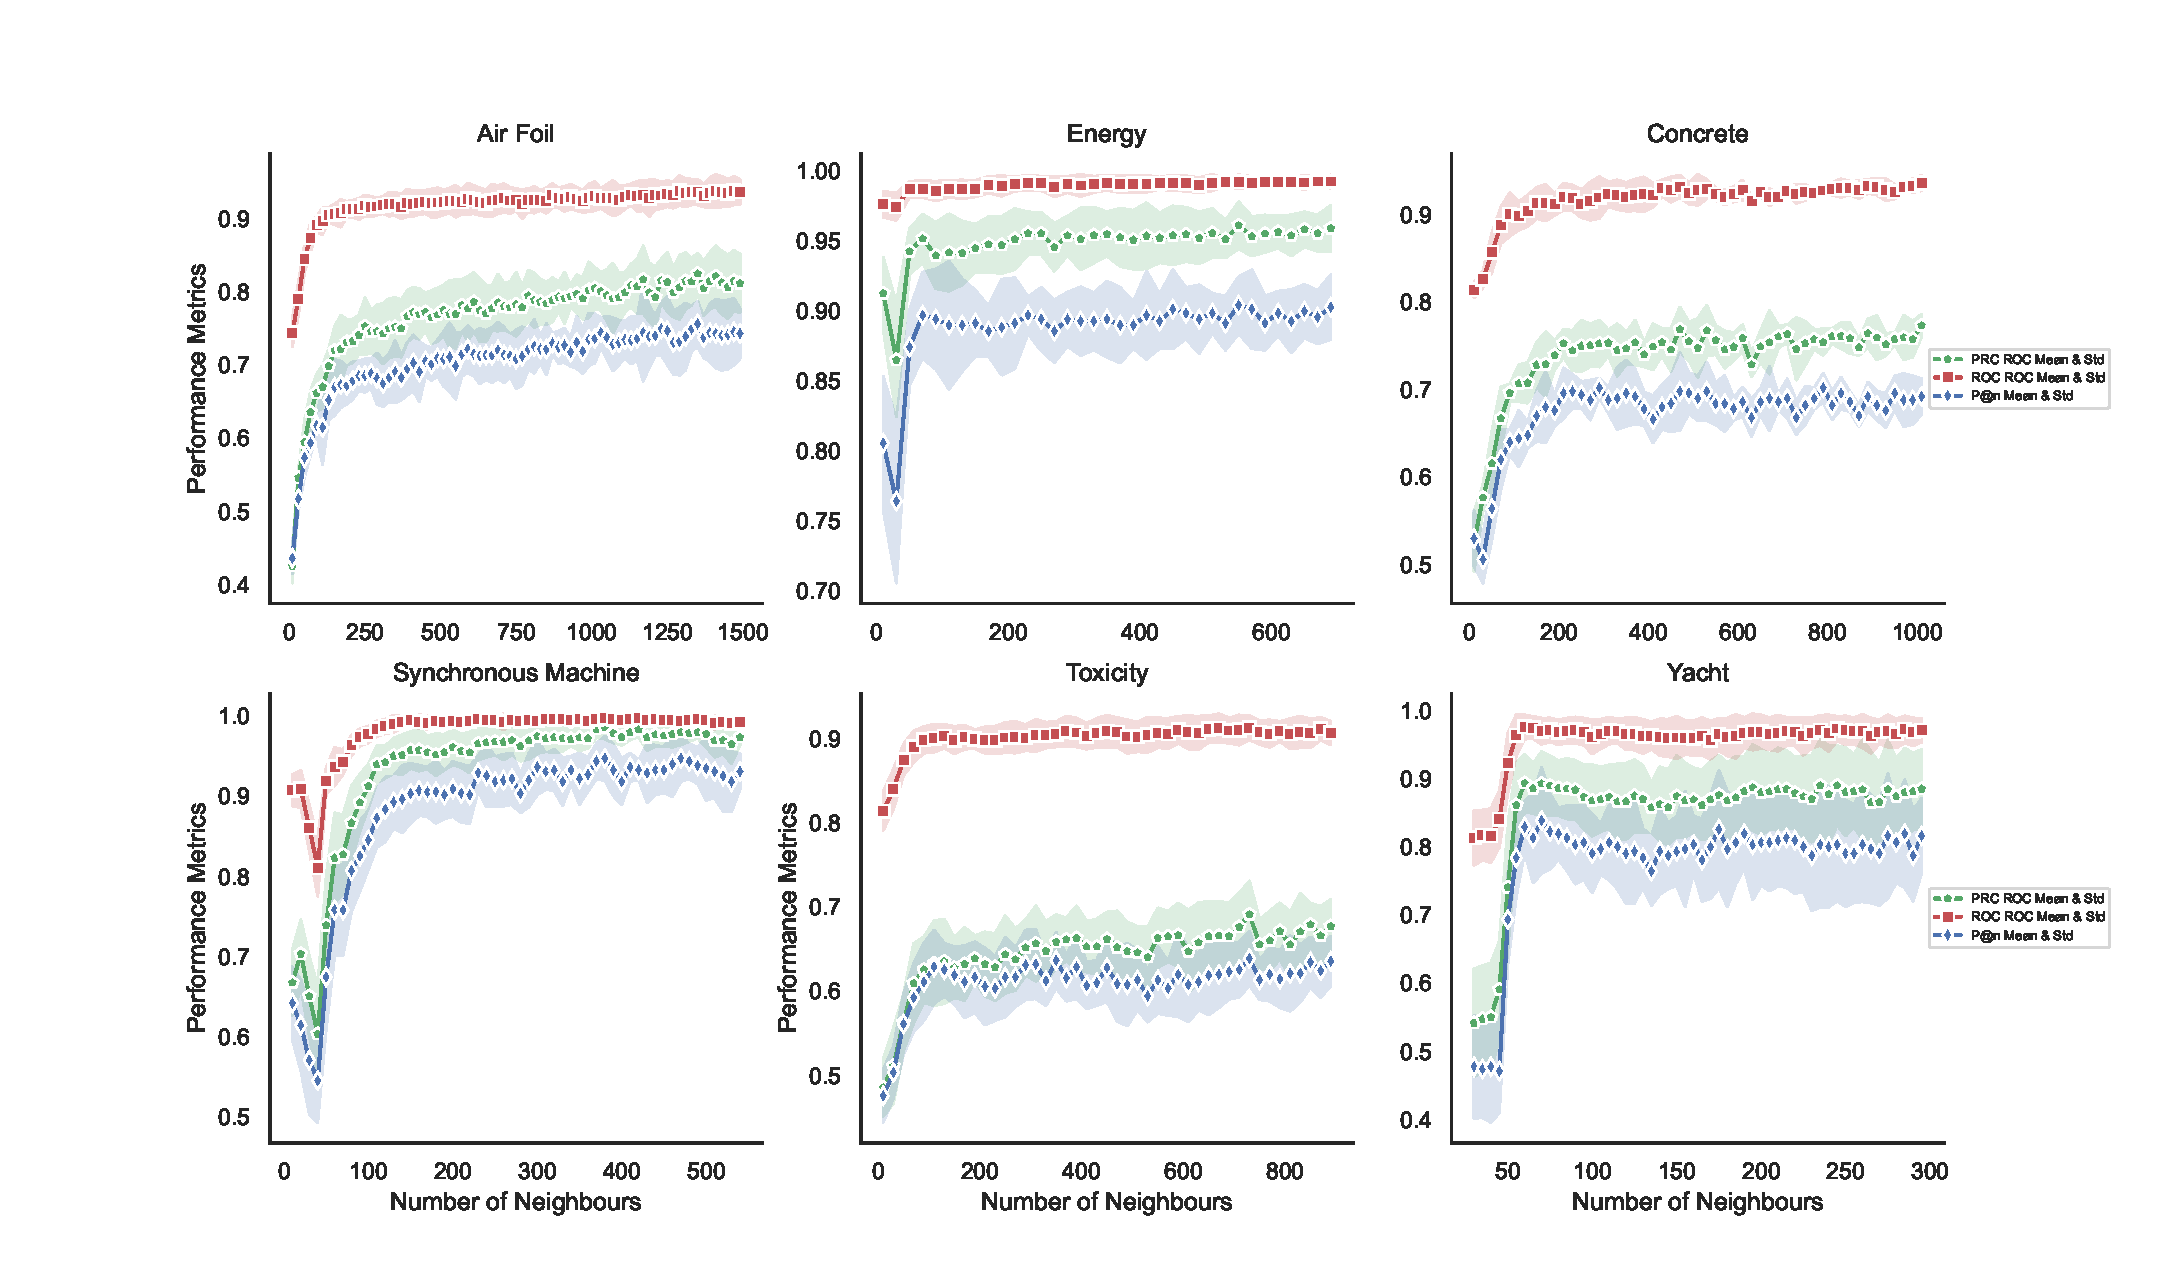
\includegraphics[width=12cm]{images/Pic_sensitivity1.pdf}
\caption{Phân tích độ nhạy trên tham số $k$, trong đó các đường biểu thị giá trị trung bình và các vùng được tô bóng biểu thị độ lệch chuẩn tương ứng của từng số liệu trong các thử nghiệm độc lập 10. Việc tăng số lượng hàng xóm trước tiên sẽ cải thiện phần lớn hiệu suất về mặt PRC AUC (đường màu xanh lá cây có dấu hoa thị), ROC AUC (đường màu đỏ có hình vuông) và Precision@n (đường màu xanh có hình kim cương), sau đó mang lại mức tăng hiệu suất không đáng kể. }\label{fig:sensitivity1}
\end{figure}
\section{Nghiên cứu cắt bỏ}
\label{Appendix:Ablation}
\subsection{Tỷ lệ độ dài khoảng thời gian phân vị có điều kiện}

Trong phần phương pháp của chúng tôi, chúng tôi đã xác định độ dài khoảng phân vị có điều kiện phù hợp cho một quan sát $b^{q}$ khi $b^{q} > \tau_{100}^{q}$ hoặc $ b^{q} <\tau_{0}^{q}$ như trong Phương trình (4). Chúng tôi xác định độ dài khoảng phù hợp cho $b^{q}$ dựa trên $\mathrm{max}(w(\mathbf{x}\rvert\mathbf{b}^{q}))$ và mở rộng quy mô hơn nữa bằng cách xem xét khoảng cách của nó với $\tau_{100}^{q}$ hoặc $\tau_{0}^{q}$. Ngoài ra, chúng ta có thể chỉ cần xác định độ dài khoảng phù hợp là $\mathrm{max}(w(\mathbf{x}\rvert\mathbf{b}^{q}))$ mà không cần chia tỷ lệ. Nói cách khác, chúng ta có thể coi tất cả các quan sát nằm bên ngoài $[\tau_{0}^{q}, \tau_{100}^{q}]$ là như nhau. Tuy nhiên, như được hiển thị trong Hình \ref{fig:ablation1}, điều này sẽ dẫn đến sự suy giảm hiệu suất lớn về PRC AUC và Precision@n đối với hầu hết các tập dữ liệu.Cụ thể, Hình \ref{fig:ablation1} cho thấy sự khác biệt của các chỉ số hiệu suất, tức là PRC ROC, ROC AUC và Precision@n giữa việc chia tỷ lệ $\mathrm{max}(w(\mathbf{x}\rvert\mathbf{b}^{q}))$ có xem xét khoảng cách đến $\tau_{100}^{q}$ hoặc $\tau_{0}^{q}$ và không chia tỷ lệ $\mathrm{max}(w(\mathbf{x}\rvert\mathbf{b}^{q}))$. Đối với tất cả các tập dữ liệu, sự khác biệt là tích cực.
Đặc biệt, những khác biệt này rất lớn về mặt PRC AUC và Precision@n đối với hầu hết các tập dữ liệu như Năng lượng, Viêm gan, Bệnh nhân Gan Ấn Độ, 5 tổng hợp và 10 tổng hợp. Do đó, điều quan trọng là xác định độ dài khoảng phù hợp bằng cách xem xét khoảng cách tương ứng từ $b^{q}$ đến $\tau_{100}^{q}$ hoặc $\tau_{0}^{q}$ khi $b^{q}> \tau_{100}^{q}$ hoặc $b^{q}<\tau_{0}^{q}$.

\begin{figure}[!htbp]
\centering
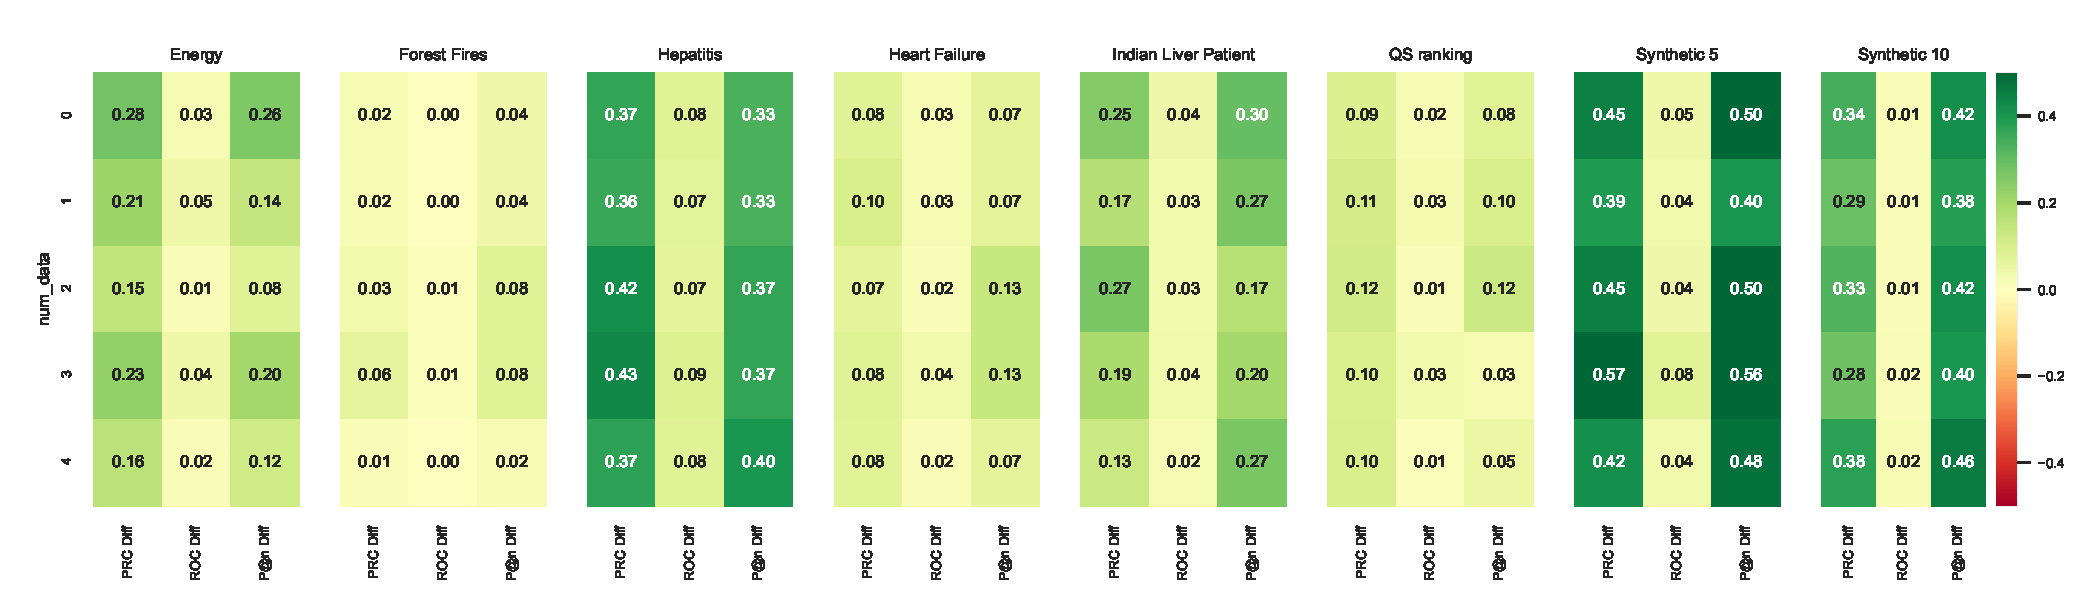
\includegraphics[width=12cm]{images/Pic_ablation1.pdf}
\caption{Hiệu ứng của việc chia tỷ lệ độ dài khoảng phân vị có điều kiện phù hợp. Đối với mỗi tập dữ liệu, kết quả thu được bằng cách thực hiện các thử nghiệm độc lập 5 về việc chèn các điểm bất thường theo ngữ cảnh. Đối với mỗi thử nghiệm, được biểu thị bằng trục y (cụ thể là $num\_data$), kết quả là sự khác biệt (theo PRC AUC, ROC AUC, Precision@n, tương ứng) của các phương pháp có hoặc không chia tỷ lệ độ dài khoảng phân vị có điều kiện phù hợp. Sự khác biệt lớn trên hầu hết các bộ dữ liệu cho thấy tầm quan trọng quan trọng của việc chia tỷ lệ độ dài khoảng cách phân vị có điều kiện phù hợp. }\label{fig:ablation1}
\end{figure}

\subsection{Cắt độ dài khoảng thời gian phân vị có điều kiện}
\begin{figure}[!htbp]
\centering
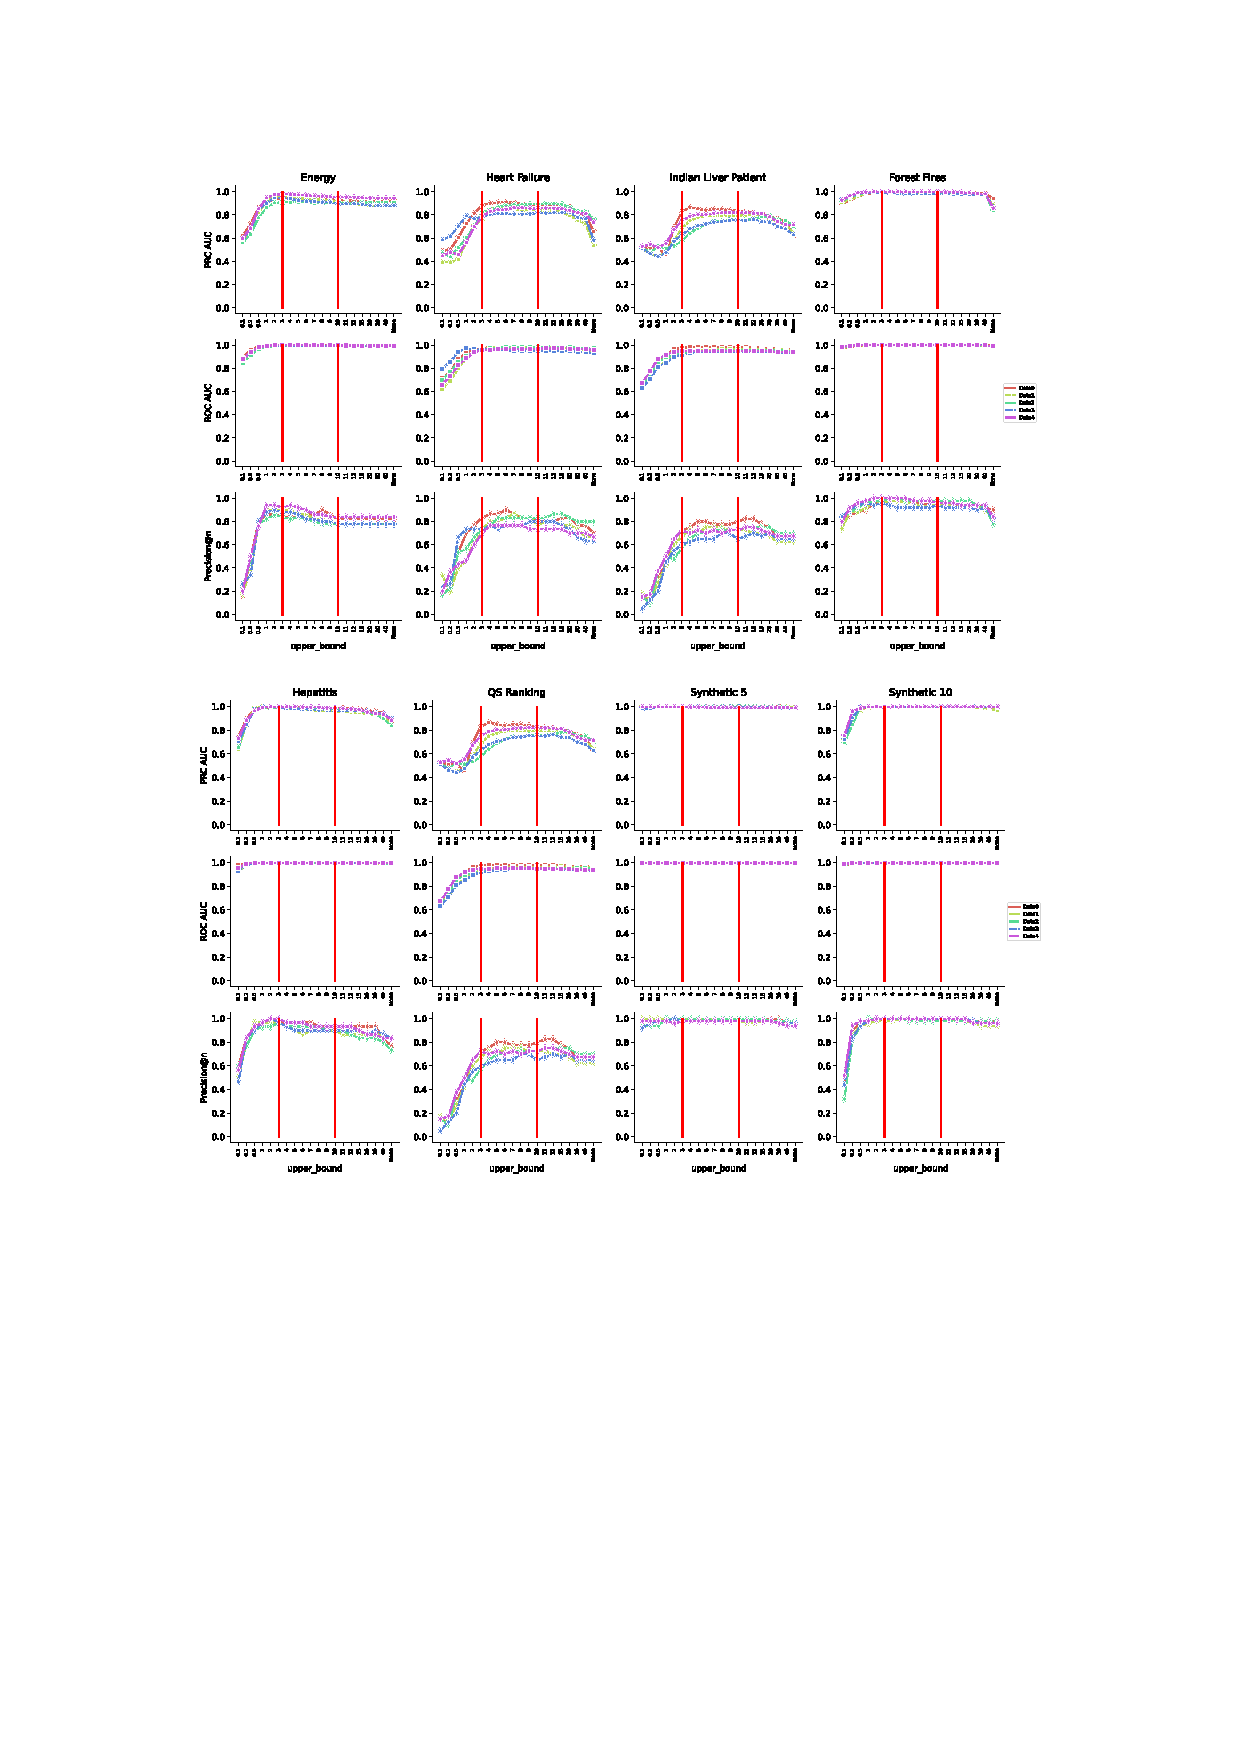
\includegraphics[width=12cm]{images/Pic_ablation2.pdf}
\caption{Hiệu ứng của việc cắt bớt độ dài khoảng phân vị có điều kiện phù hợp. Đối với mỗi tập dữ liệu, kết quả thu được bằng cách thực hiện các thử nghiệm độc lập 5 (được biểu thị bằng các đường cong khác nhau của 5) về việc chèn các bất thường theo ngữ cảnh. Sau đó, chúng tôi tính toán các số liệu hiệu suất (tức là PRC AUC, ROC AUC và Precision@n) của QCAD bằng cách thay đổi siêu tham số $\eta$ trong $\{0.1,0.2,0.5,1,2,3,...,11,12,15,20,30,40,None\}$, trong đó \textit{None} có nghĩa là không thực hiện cắt. Trên hầu hết các tập dữ liệu, hiệu suất tốt nhất đạt được khi sử dụng $3<\eta<10$, như được hiển thị bằng hai đường thẳng đứng màu đỏ.}\label{fig:ablation2}
\end{figure}

Để giảm thiểu \textit{hiệu ứng độc tài}, chúng tôi đã đề xuất cắt bớt độ dài khoảng phân vị có điều kiện phù hợp lớn với giới hạn trên, được đặt thành $\frac{\eta}{100}$. Cụ thể hơn, chúng tôi đặt $\eta=10$. Để chứng minh tính hiệu quả của chiến lược này trên các tập dữ liệu khác nhau, chúng tôi tính toán số liệu hiệu suất của QCAD bằng cách thay đổi siêu tham số $\eta \in \{0.1,0.2,0.5,1,2,3,...,11,12,15,20,30,40,None\}$, trong đó \textit{None} có nghĩa là không thực hiện cắt bớt.Như được hiển thị trong Hình \ref{fig:ablation2}, việc tăng $\eta$ sẽ dẫn đến các giá trị PRC AUC, ROC AUC và Precision@n cao hơn khi $\eta$ nhỏ (tức là nhỏ hơn $1$ đối với hầu hết các tập dữ liệu). Tiếp theo, một mặt, ROC AUC vẫn ổn định khi $\eta$ tăng, ngay cả khi không bị cắt (tức là $\eta=None$). Nói cách khác, chiến lược cắt bớt không ảnh hưởng đến số liệu ROC AUC. Mặt khác, PRC AUC và Precision@n dần dần đạt đến mức ổn định khi $\eta$ tăng lên. Sau một khoảng thời gian nhất định, PRC AUC và Precision@n bắt đầu giảm với mức tăng $\eta$. Nhìn chung, trên hầu hết các tập dữ liệu, PRC AUC và Precision@n thường đạt được giá trị cao hơn với $3\leq \eta \leq 10$ so với các tập dữ liệu không cắt bớt. Do đó, các hiệu ứng độc tài \textit{thực sự} tồn tại và chúng chủ yếu
giảm hiệu suất của QCAD về mặt PRC AUC và Precision@n. Hơn nữa, chiến lược cắt được đề xuất của chúng tôi có thể khắc phục vấn đề này một cách hiệu quả.

\end{document}
